
\documentclass[12pt,a4paper]{article}

% ====== PAQUETES BÁSICOS ======
\usepackage[spanish]{babel}
\usepackage[utf8]{inputenc}
\usepackage[T1]{fontenc}
\usepackage{graphicx}
\usepackage{float}
\usepackage{amsmath, amssymb}
\usepackage{booktabs}
\usepackage{hyperref}
\usepackage{geometry}
\geometry{margin=2.5cm}
\usepackage{caption}
\usepackage{subcaption} % <— para figuras lado a lado
\usepackage{fancyhdr}

% --- para tablas y texto en monoespaciado con cortes
\usepackage{tabularx}
\usepackage{array}
\usepackage{ragged2e}
\usepackage{seqsplit}
\usepackage{microtype}

\newcolumntype{Y}{>{\RaggedRight\arraybackslash}X}
\newcolumntype{L}[1]{>{\RaggedRight\arraybackslash}p{#1}}
\newcommand{\code}[1]{\texttt{\seqsplit{#1}}}
\setlength{\tabcolsep}{6pt}
\renewcommand{\arraystretch}{1.12}

% ====== ENCABEZADO ======
\pagestyle{fancy}
\fancyhf{}
\lhead{TD VI – Inteligencia Artificial}
\rhead{Trabajo Práctico III}
\cfoot{\thepage}

% ====== PORTADA ======
\title{\vspace{-2cm}\textbf{Trabajo Práctico III: Clasificación de Audio}\\[0.2cm]
\large Tecnología Digital VI: Inteligencia Artificial}
\author{Facundo Amaya \and Juan Ignacio Elosegui \and Nicolás Boudourian}
\date{Universidad Torcuato Di Tella \\ Noviembre 2025}

\begin{document}
\maketitle
\thispagestyle{empty}
\vspace{1cm}

\begin{abstract}
\noindent
Implementamos un sistema de clasificación de comandos de voz con el conjunto \textit{Speech Commands} de Google (grabaciones de \(\sim\)1 segundo) para diez clases (\texttt{yes, no, up, down, left, right, on, off, stop, go}). El foco del trabajo es \textbf{entender el efecto de los hiperparámetros} en el desempeño y la estabilidad del entrenamiento, comparando arquitecturas (MLP y CNN), representaciones (WAV vs. Mel-espectrogramas), funciones de activación, optimizadores, esquemas de entrenamiento y regularización. Todas las corridas se registraron en Weights \& Biases (W\&B) con sus métricas y metadatos.
\end{abstract}

\newpage

% ==============================================================
\section*{Ejercicio 1 — Configuración}
\subsection*{Desarrollo}
\noindent
Entorno de ejecución: Google Colab y máquinas locales (macOS/Windows). Dependencias principales: \texttt{torch}, \texttt{torchaudio}, \texttt{soundfile}, \texttt{wandb}, \texttt{tqdm}. Se parametrizó por \(\{\) \texttt{SEED=42}, \texttt{SR=16000 Hz}, \texttt{N\_MELS=32}, \texttt{BATCH\_SIZE=128}, \texttt{EPOCHS=25–50}, \texttt{LR=1e-3} \(\}\), con detección de dispositivo (\texttt{CUDA/MPS/CPU}) y descarga automática del dataset si no está presente.\\
\textbf{Registro en W\&B}: cada experimento almacena hiperparámetros y métricas \texttt{train\_loss}, \texttt{val\_loss}, \texttt{train\_acc}, \texttt{val\_acc} por época.

\subsection*{Gráficos}
\begin{figure}[H]\centering
  \begin{subfigure}{0.48\textwidth}\centering
    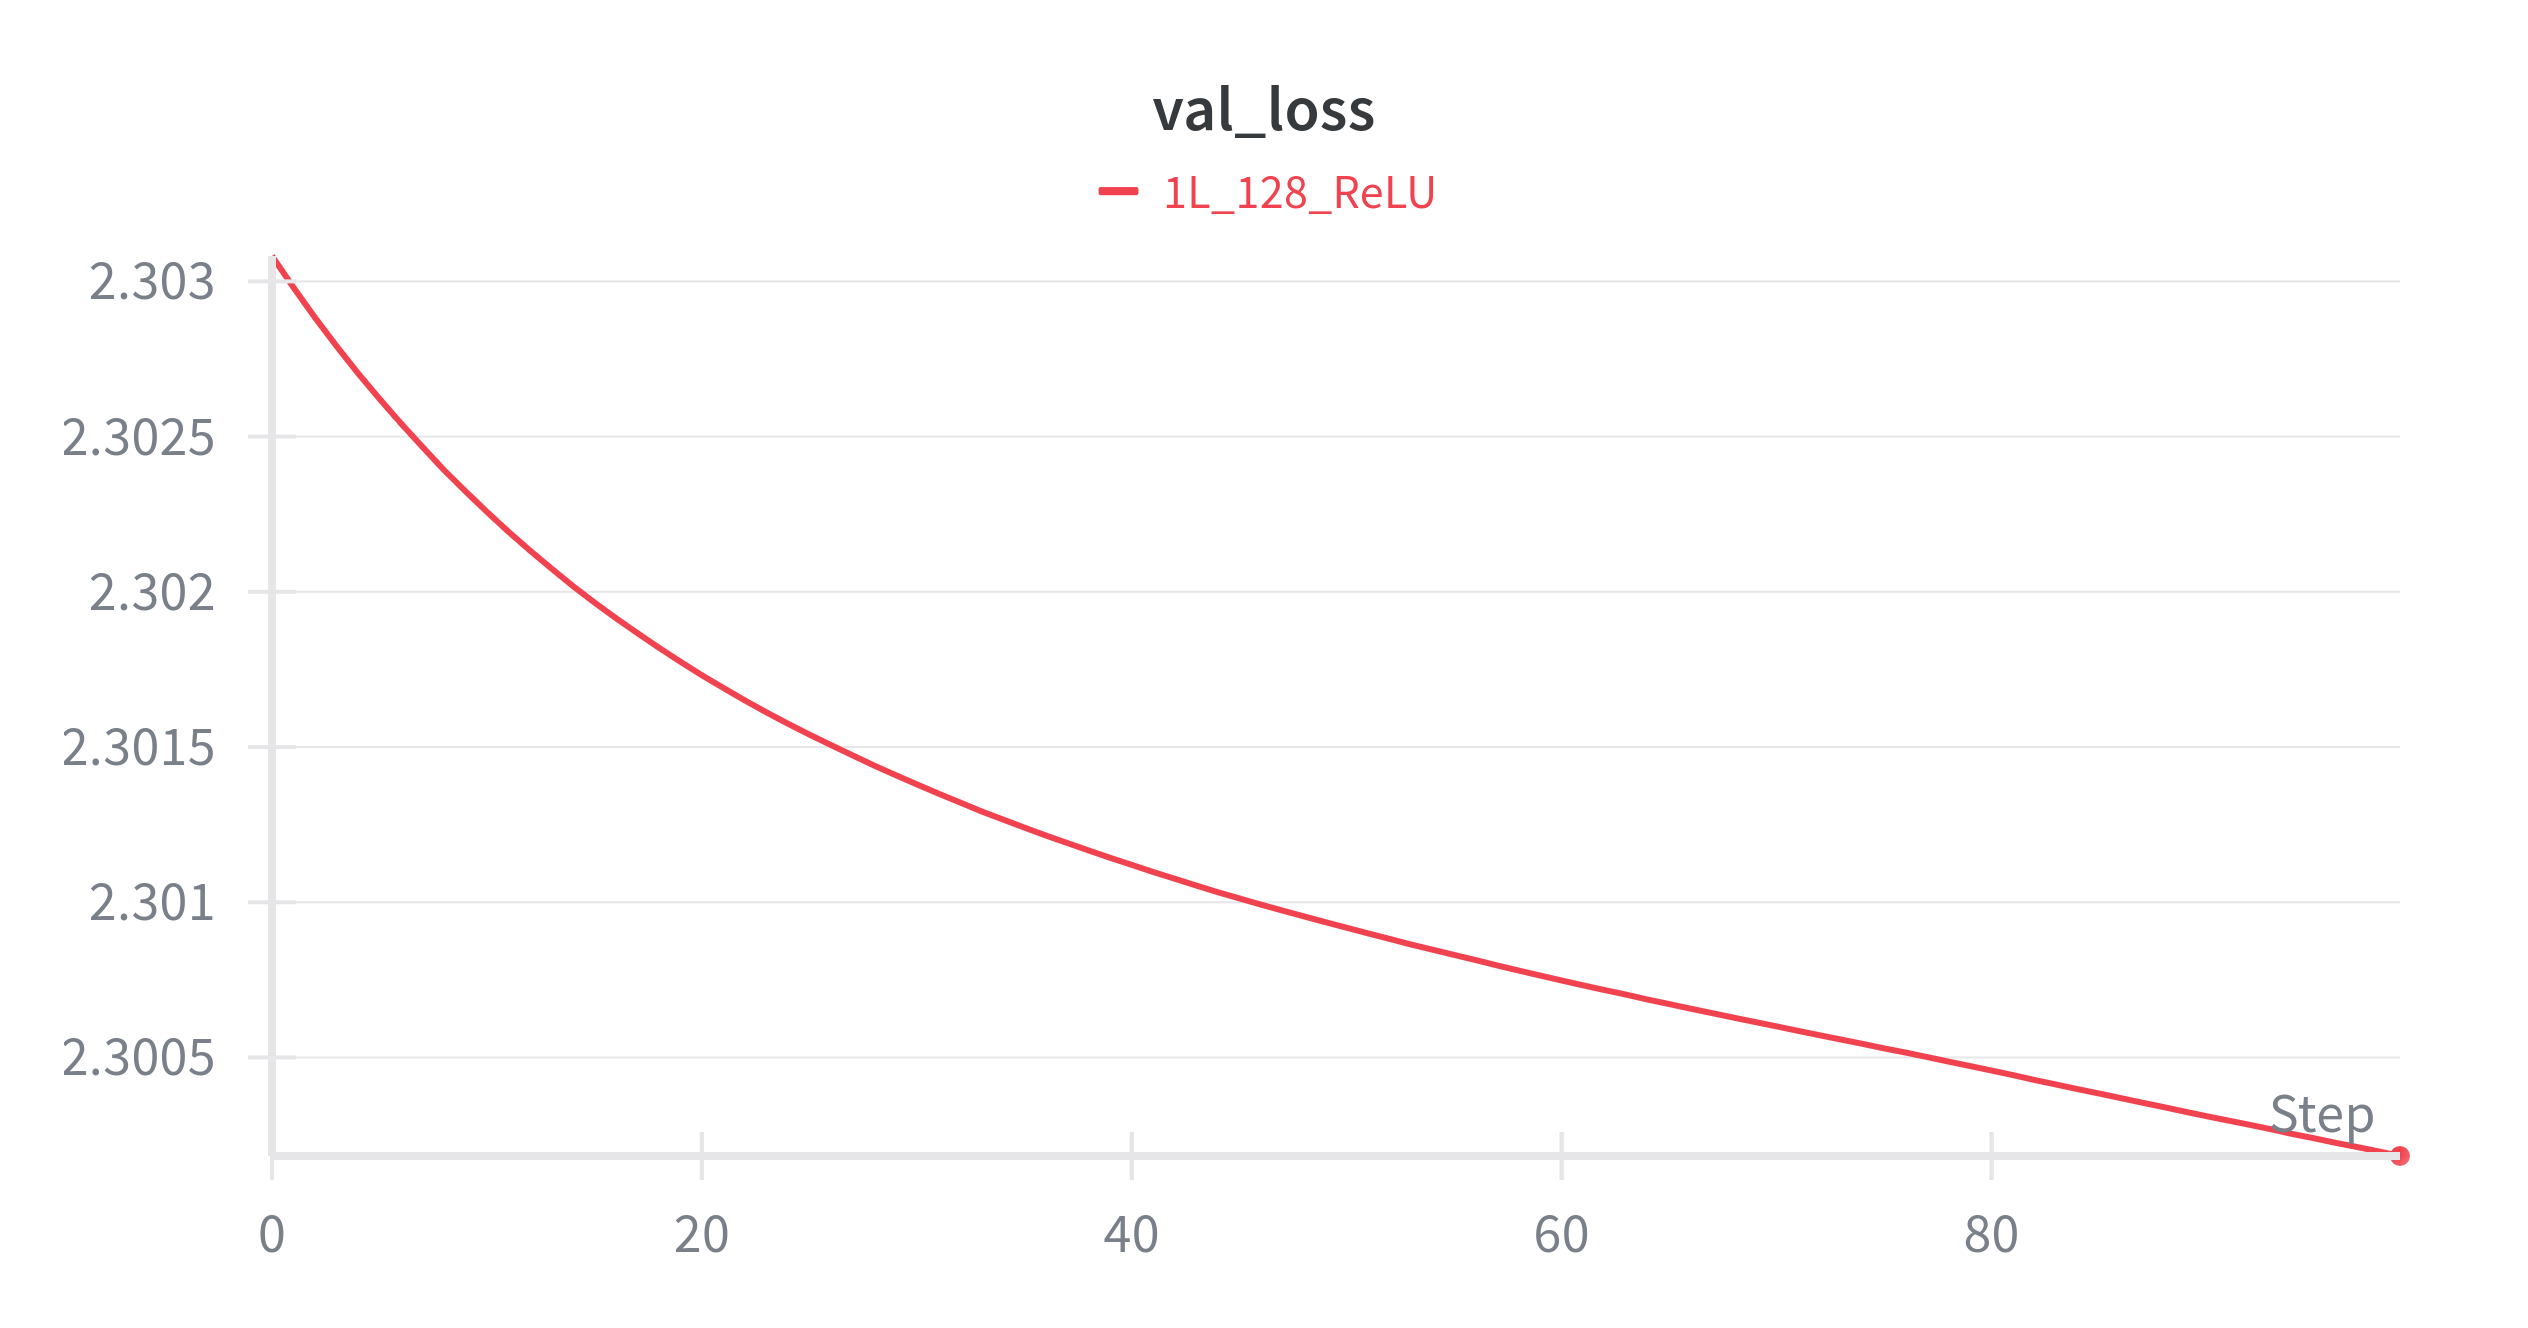
\includegraphics[width=\linewidth]{figs/1-val_loss.png}
    \caption{Validación — Loss}
  \end{subfigure}\hfill
  \begin{subfigure}{0.48\textwidth}\centering
    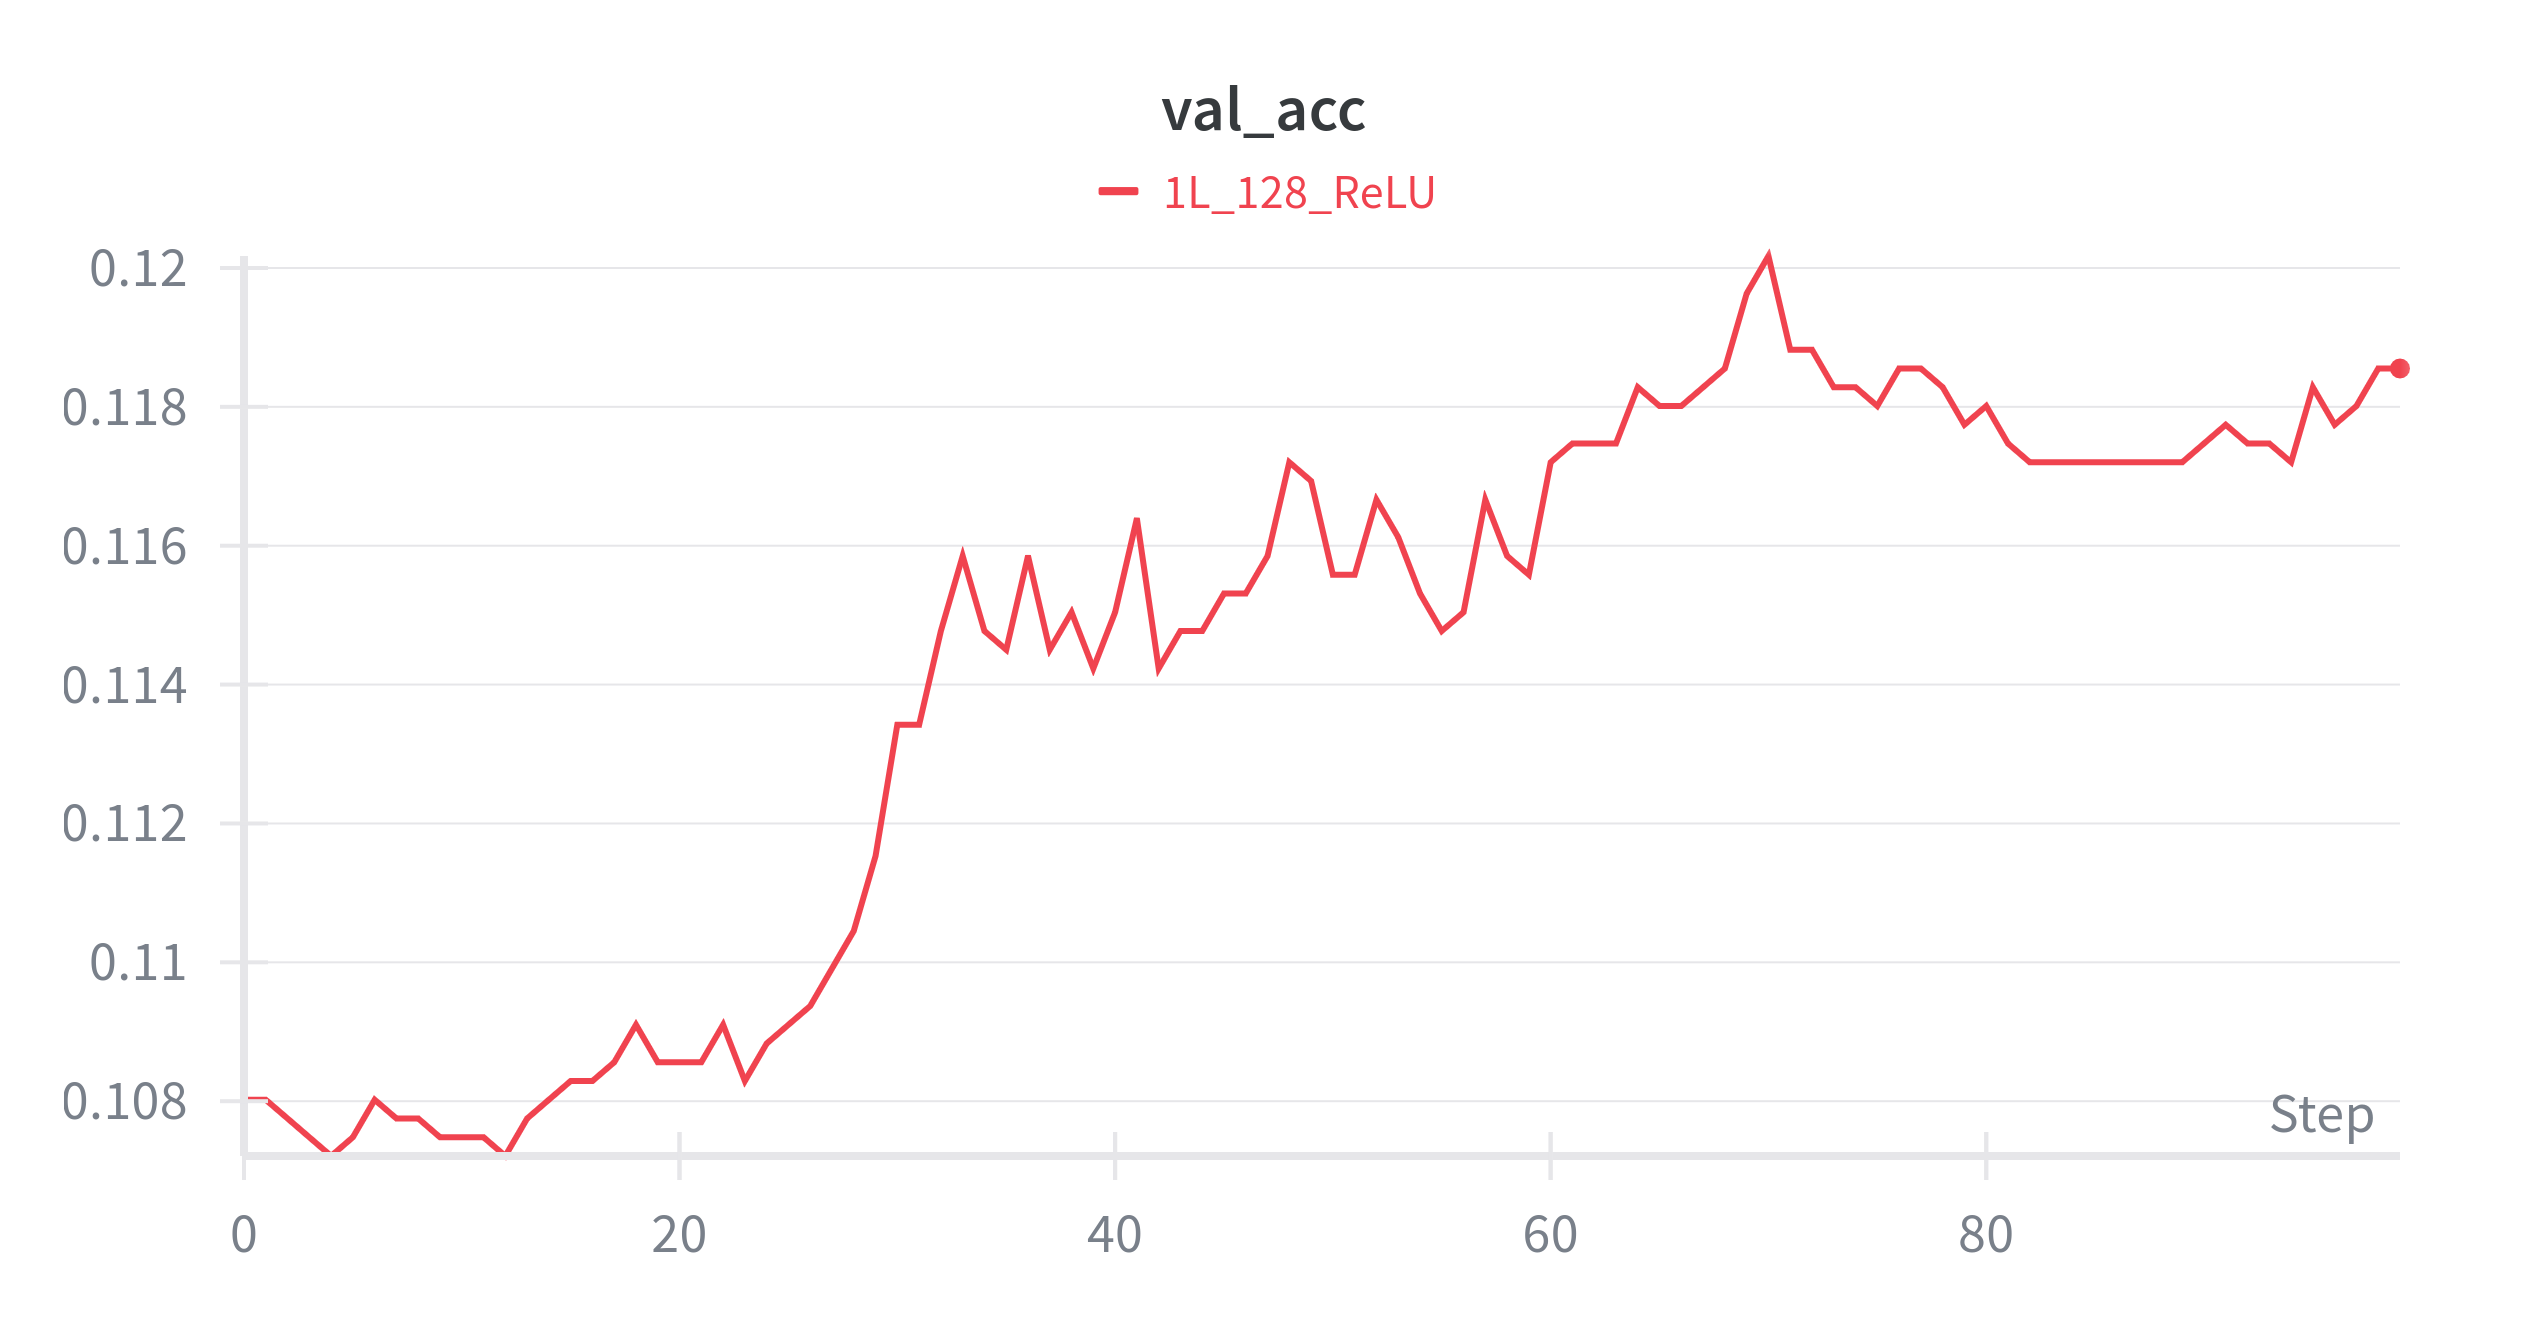
\includegraphics[width=\linewidth]{figs/1-val_acc.png}
    \caption{Validación — Accuracy}
  \end{subfigure}
  \caption{Evolución de métricas del baseline (Ej.1).}
\end{figure}

\noindent\textbf{Min/Max (W\&B).} \texttt{val\_loss} desciende de \(\approx 2.303\) a \(\approx 2.300\). \texttt{val\_acc} sube de \(\approx 0.106\) a \(\approx 0.120\).\\
\textbf{Lectura.} Mejora marginal esperable para un baseline simple; sin señales de overfitting.

% ==============================================================
\section*{Ejercicio 2 — Arquitectura (MLP)}
\subsection*{Desarrollo}
\noindent
Se evaluaron MLPs variando la profundidad (2-4 capas ocultas) y ancho (64, 128, 256, neuronas). En cuanto al \textit{accuracy} vemos que el pico se encuntra en 0.12 y el piso en 0.106. Si nos referimos al \textit{loss}, el máximo se encuntra en 2.303 y el minimo en 2.300.

\subsection*{Resultados (curvas)}
\begin{figure}[H]\centering
  \begin{subfigure}{0.48\textwidth}\centering
    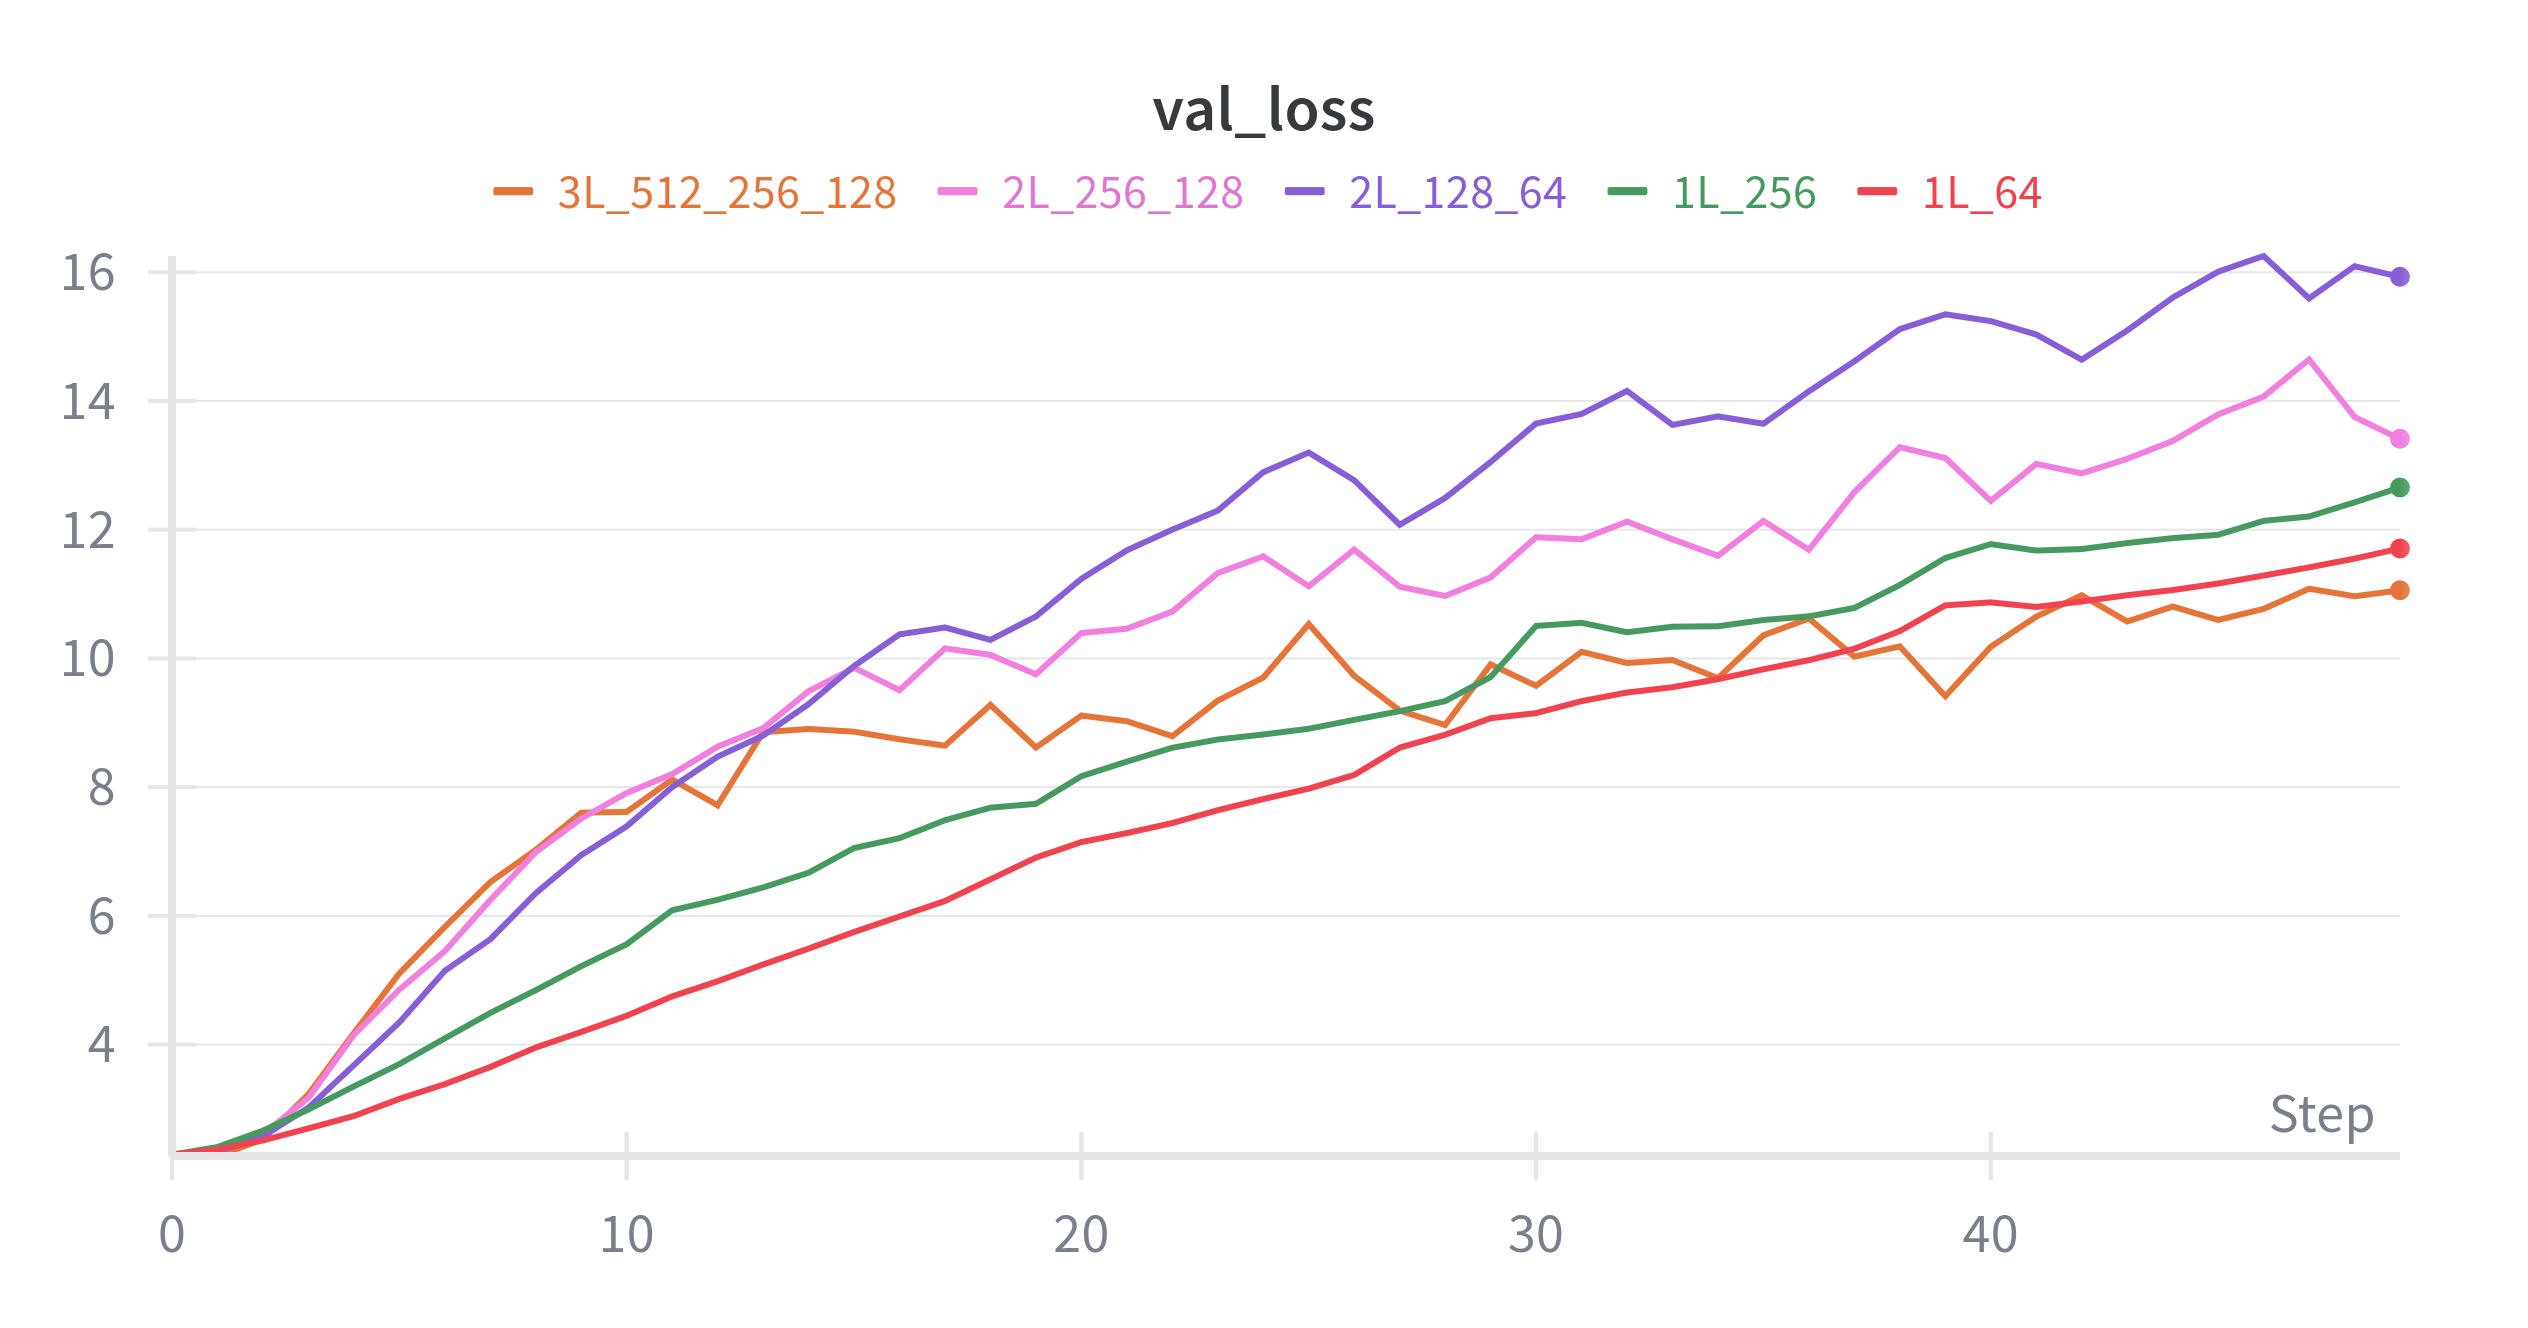
\includegraphics[width=\linewidth]{figs/2-val_loss.png}
    \caption{Validación — Loss}
  \end{subfigure}\hfill
    \begin{subfigure}{0.48\textwidth}\centering
    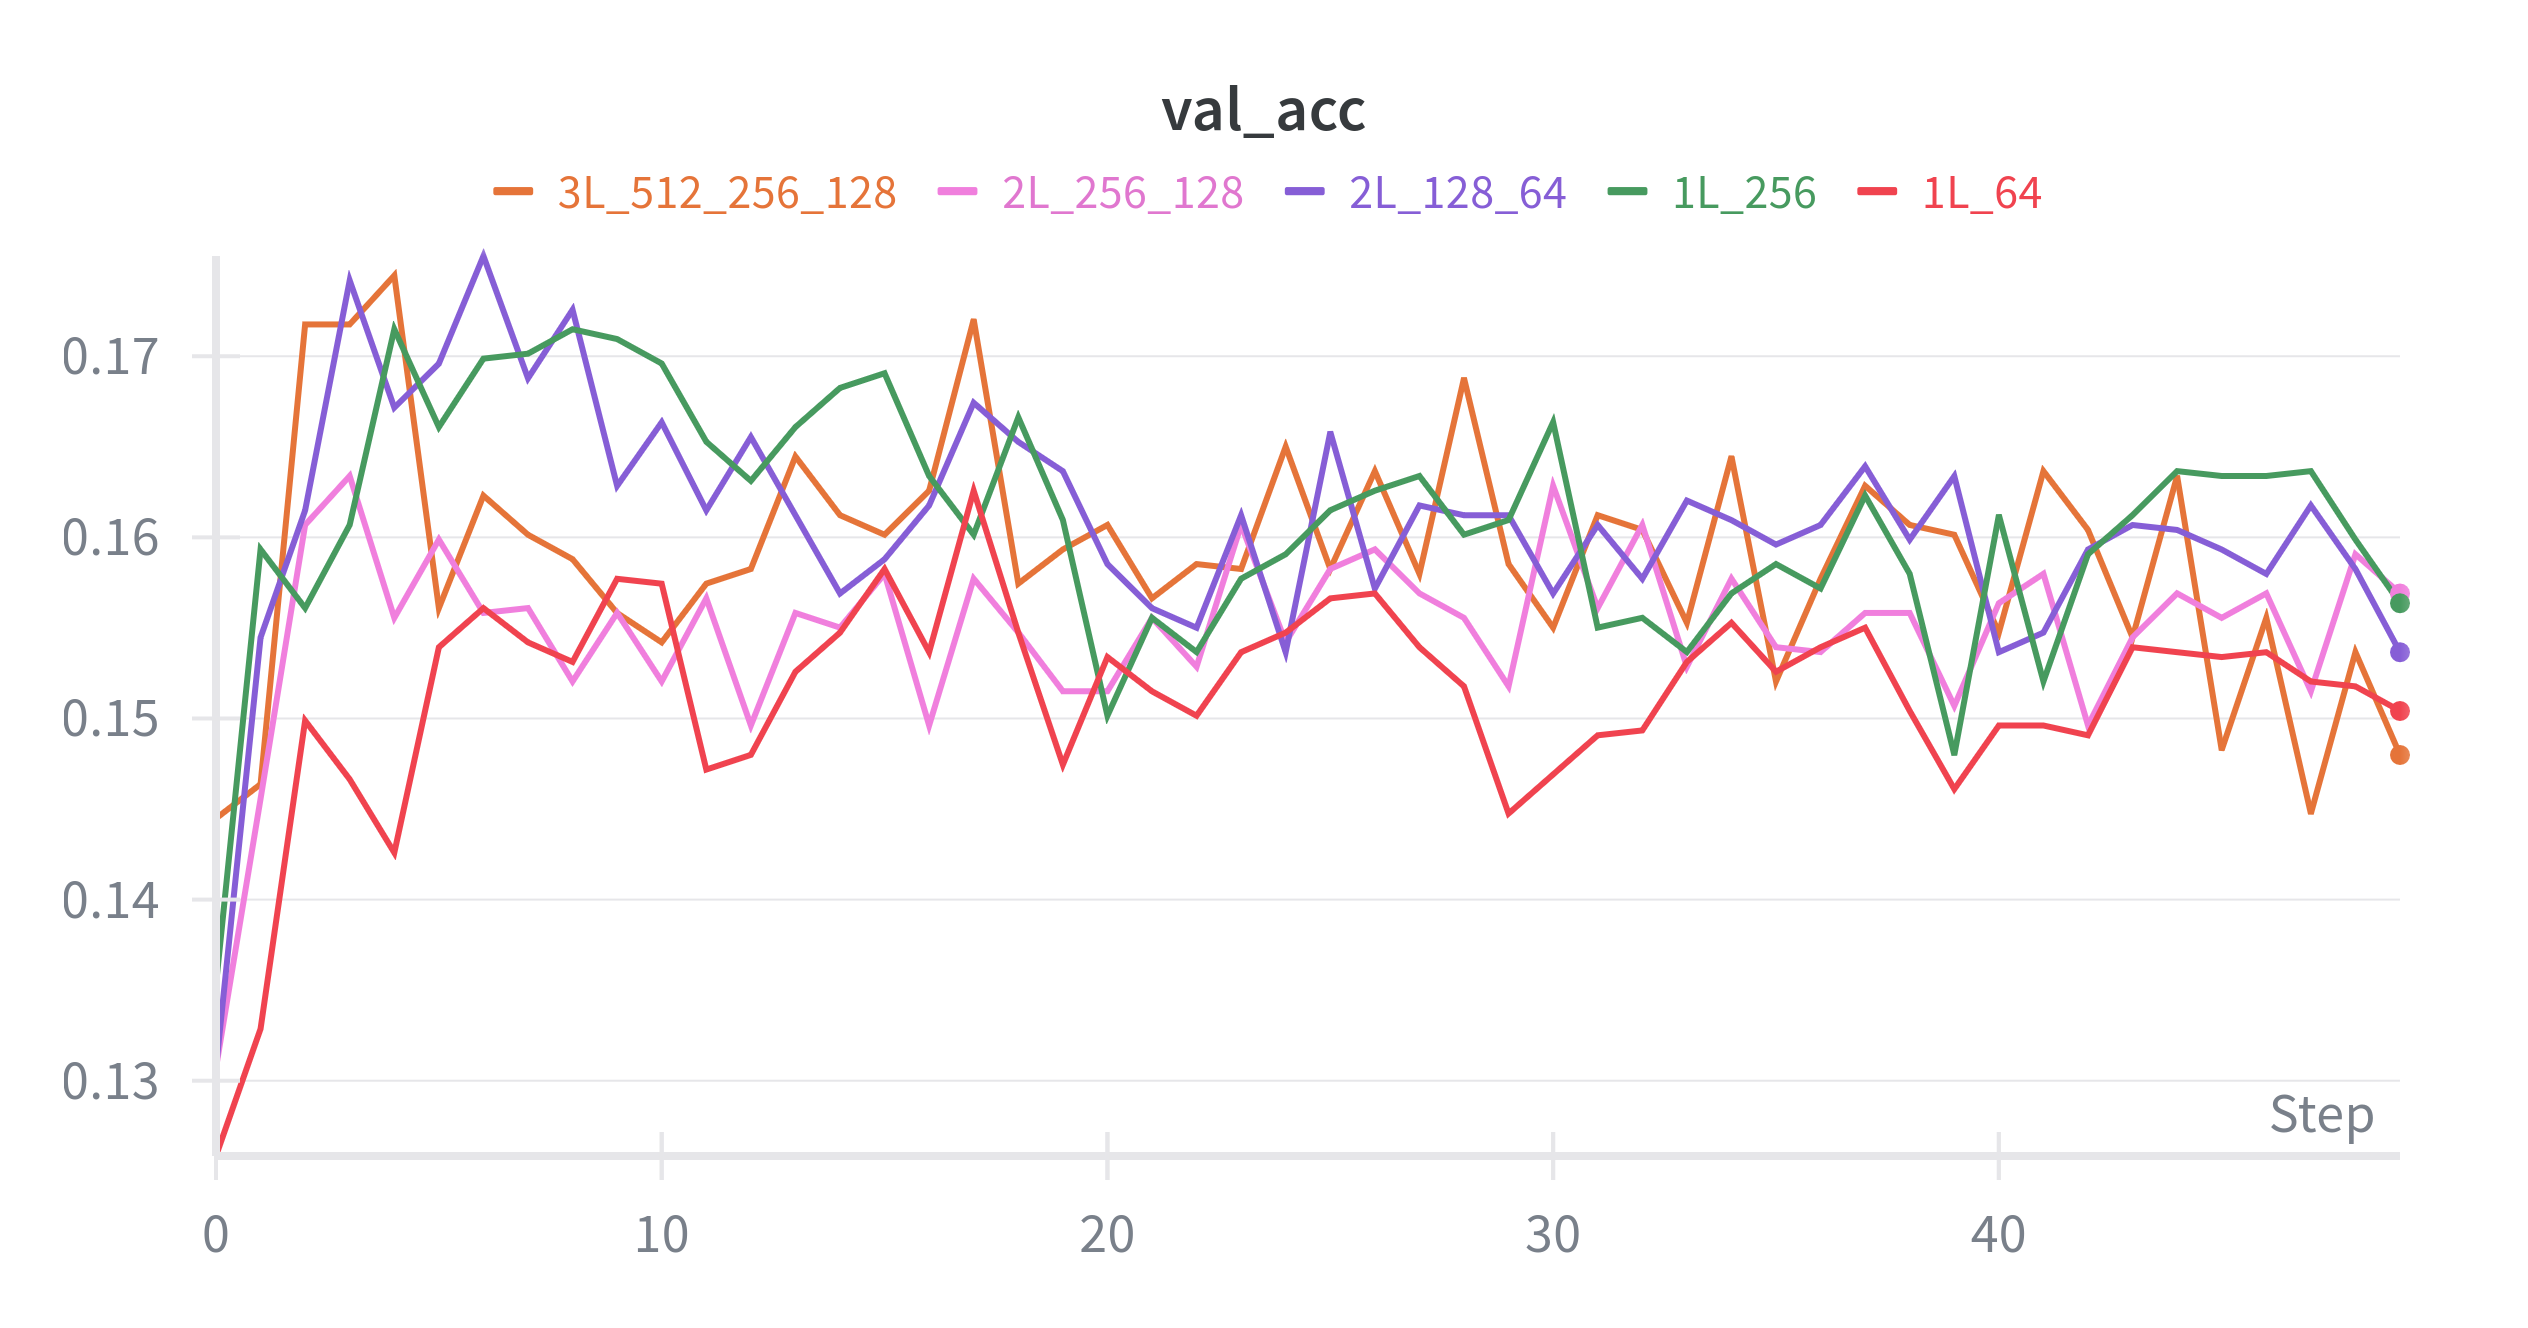
\includegraphics[width=\linewidth]{figs/2-val_acc.png}
    \caption{Validación — Accuracy}
  \end{subfigure}
  \caption{Arquitecturas MLP comparadas (Ej.2).}
\end{figure}

\noindent\textbf{Min/Max (W\&B).} \texttt{val\_loss} \(\in [\approx 2.300,\; \approx 2.303]\); \texttt{val\_acc} \(\in [\approx 0.106,\; \approx 0.120]\).\\
\textbf{Lectura.} Cambiar capacidad en MLP mejora training, pero la generalización (val) casi no se mueve: \emph{underfitting} fuerte del pipeline sin inductiva temporal/frecuencial.

\subsection*{Conclusión}
\noindent Un MLP mediano (3 capas con 128 neuronas) balanceó bien sesgo–varianza, maximizando \texttt{val\_acc} sin degradar \texttt{val\_loss}. Las redes más profundas no trajeron mejoras significativas y mostraron mayor separación train–val (indicio de overfitting).

% ==============================================================
\section*{Ejercicio 3 — MEL vs. WAV}
\subsection*{Desarrollo}
\noindent
Comparamos dos entradas: (i) \textbf{WAV crudo} aplanado para MLP, y (ii) \textbf{Mel-espectrogramas} (\texttt{N\_MELS = 32}) como imagen (1 canal), usados en MLP (aplanado) y en \textbf{CNN 2D}. La representación tiempo–frecuencia (MEL) preserva regularidades locales que una CNN puede explotar.

\subsection*{Resultados (curvas)}
\begin{figure}[H]\centering
  \begin{subfigure}{0.48\textwidth}\centering
    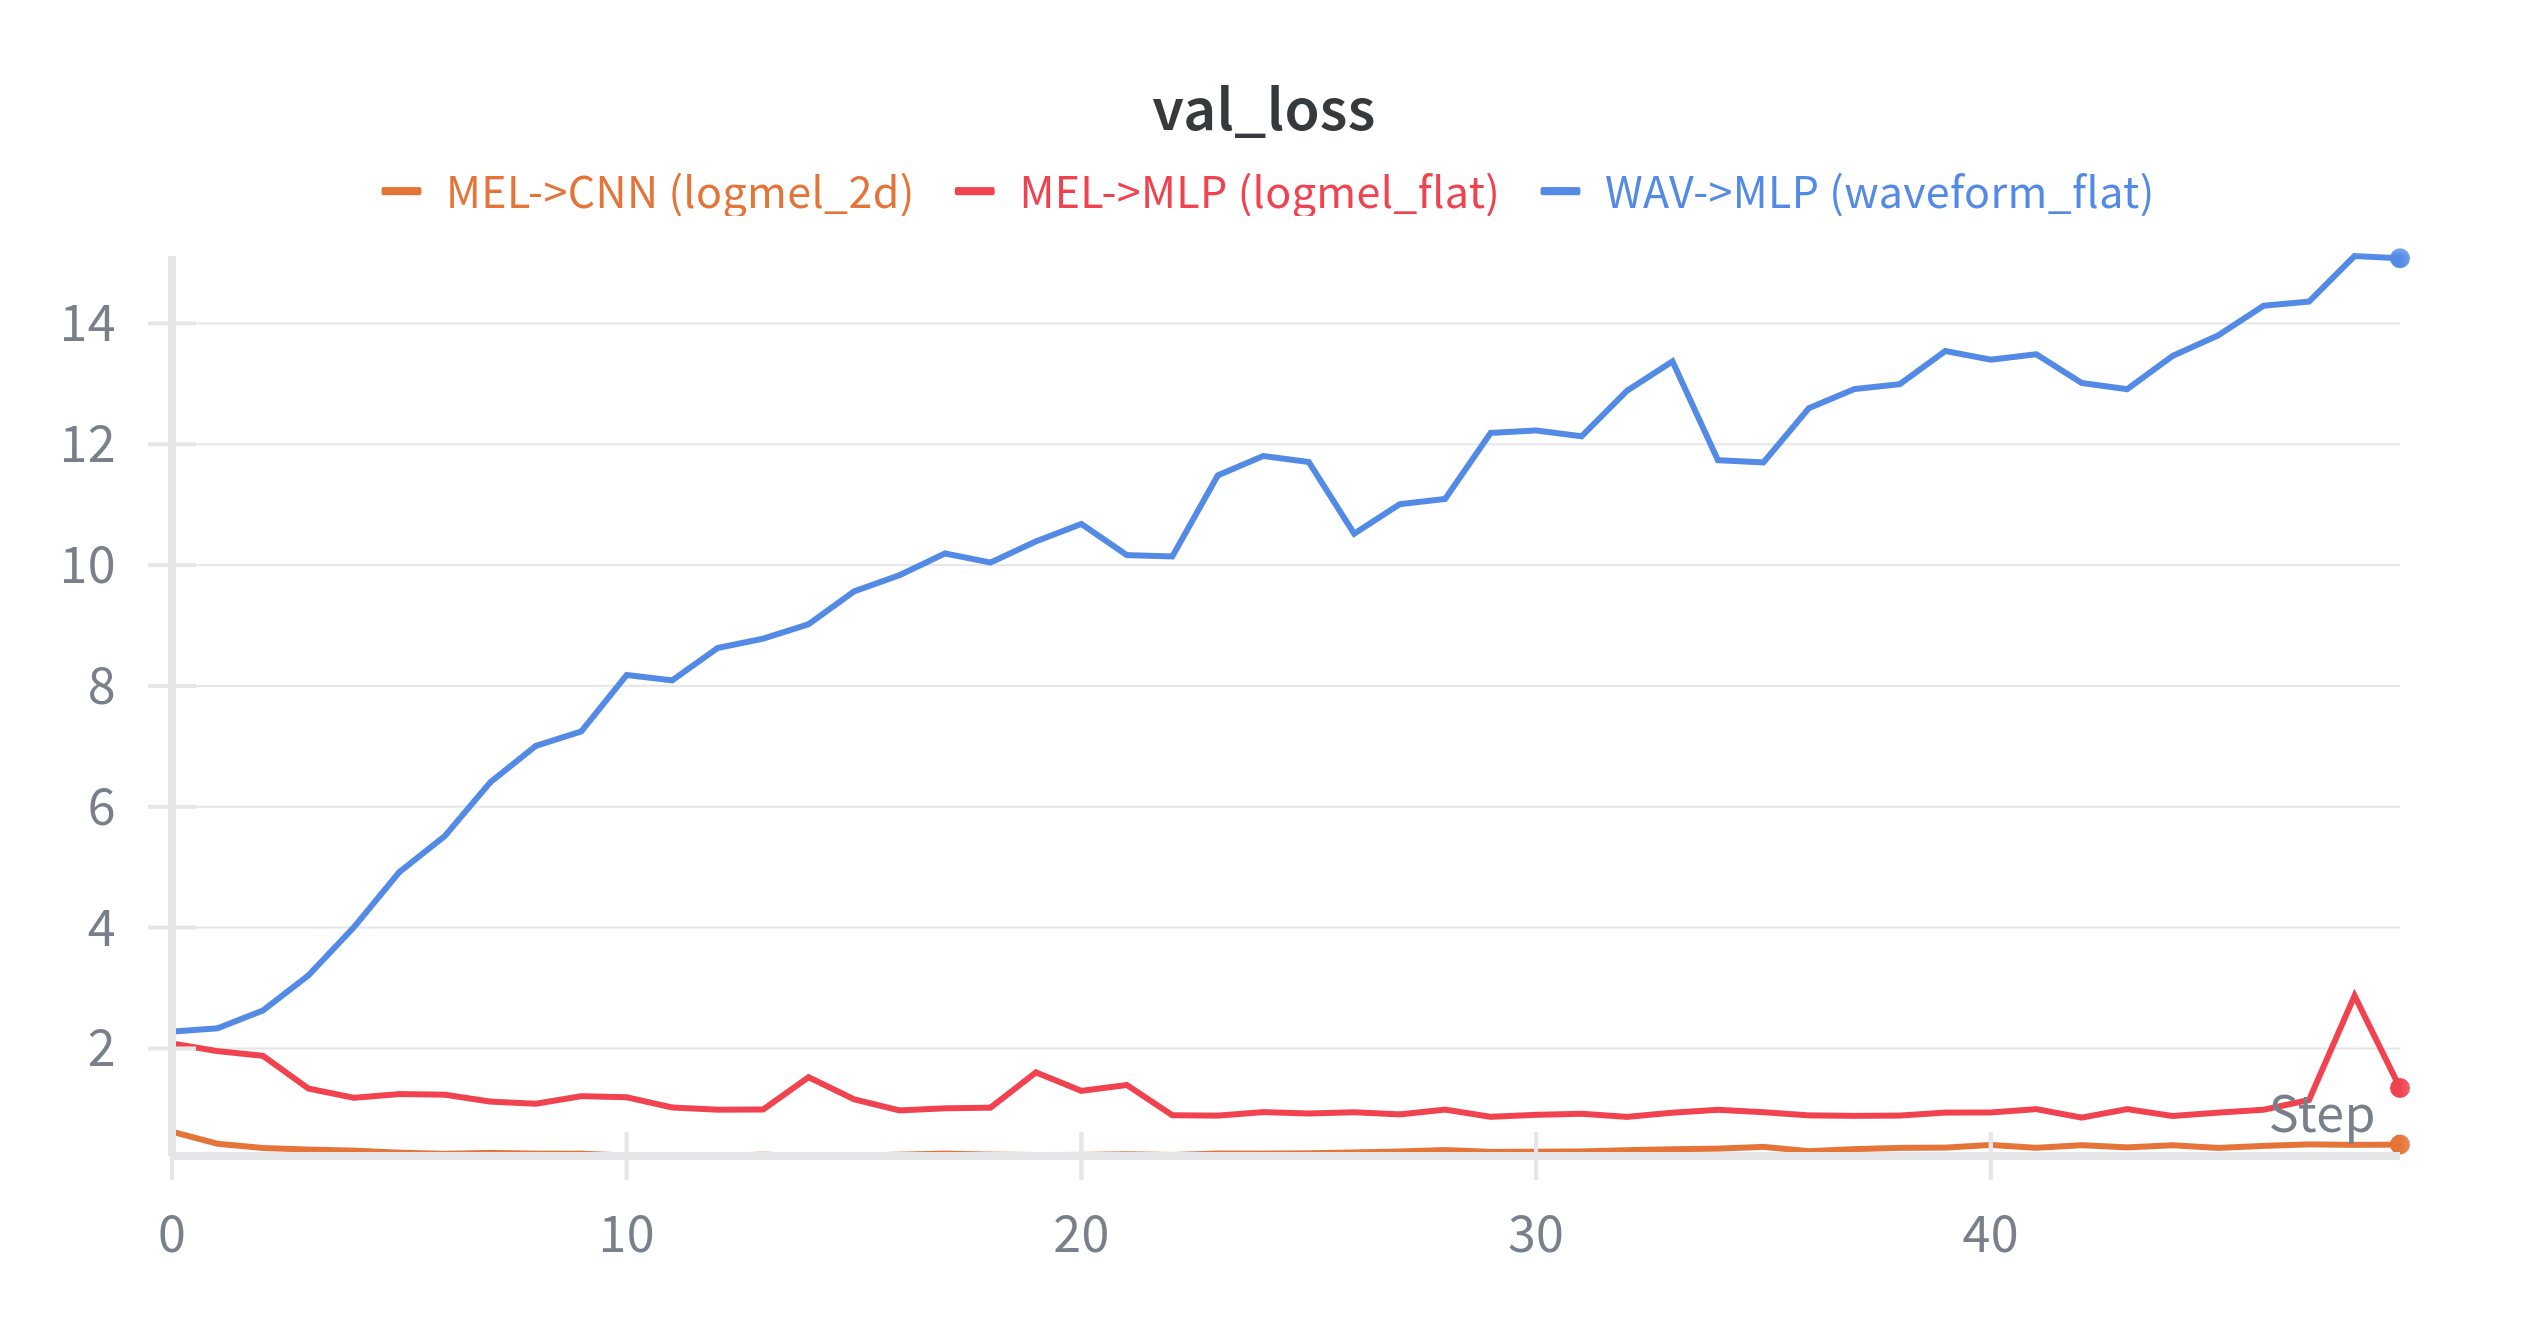
\includegraphics[width=\linewidth]{figs/3-val_loss.png}
    \caption{Validación — Loss}
  \end{subfigure}\hfill
  \begin{subfigure}{0.48\textwidth}\centering
    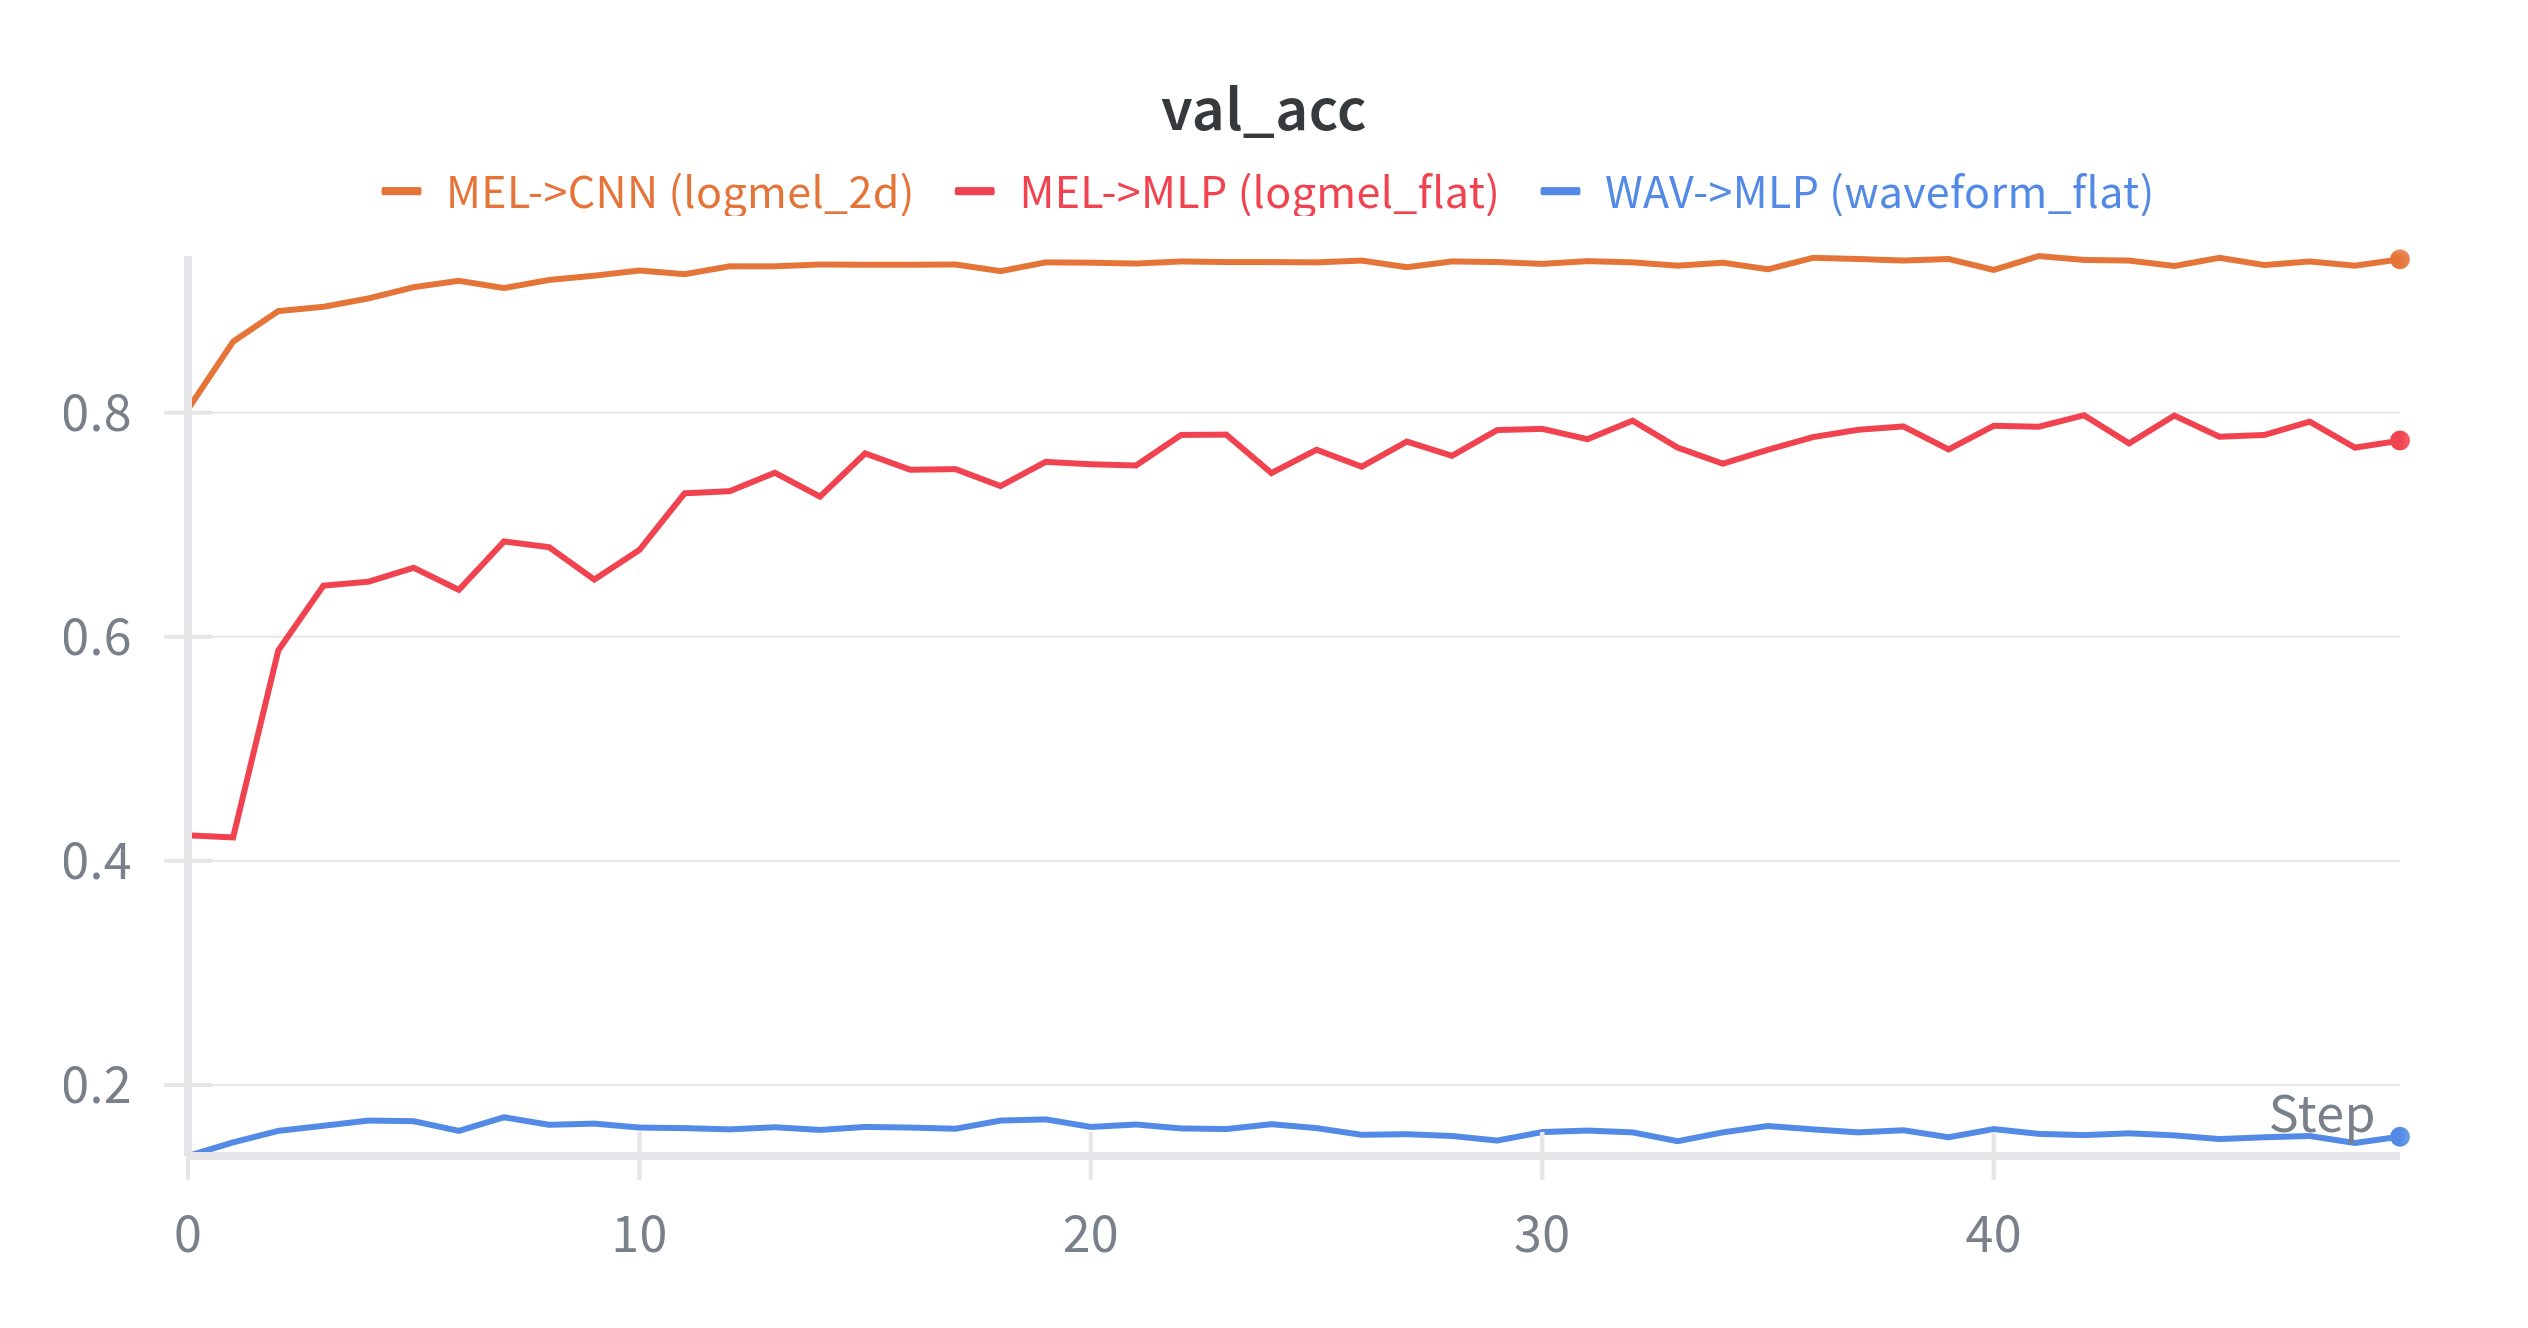
\includegraphics[width=\linewidth]{figs/3-val_acc.png}
    \caption{Validación — Accuracy}
  \end{subfigure}
  \caption{Comparación de representación/arquitectura (Ej.3).}
\end{figure}

\noindent\textbf{Min/Max (W\&B).} MEL+CNN: \texttt{val\_acc} \(\approx 0.80\)–\(0.93\), \texttt{val\_loss} \(\approx 0.25\)–\(0.60\). WAV+MLP: \texttt{val\_acc} \(\approx 0.60\)–\(0.65\), \texttt{val\_loss} \(\approx 1.0\)–\(1.4\).\\
\textbf{Lectura.} La representación MEL es decisiva; la inductiva convolucional capitaliza estructura local (tiempo–frecuencia).

\subsection*{Conclusión}
\noindent MEL mejora claramente frente a WAV crudo. La CNN sobre MEL alcanza la mayor \texttt{val\_acc} y la menor \texttt{val\_loss}, confirmando que la inductiva convolucional es adecuada para audio en dominio tiempo–frecuencia.

% ==============================================================
\section*{Ejercicio 4 — Funciones de activación}
\subsection*{Desarrollo}
\noindent
Se probaron ReLU, LeakyReLU, Tanh y Sigmoid, manteniendo arquitectura y optimizador fijos. Teóricamente, ReLU evita la saturación que sufren Tanh/Sigmoid y facilita gradientes no desvanecidos.

\subsection*{Resultados (curvas)}
\begin{figure}[H]\centering
  \begin{subfigure}{0.48\textwidth}\centering
    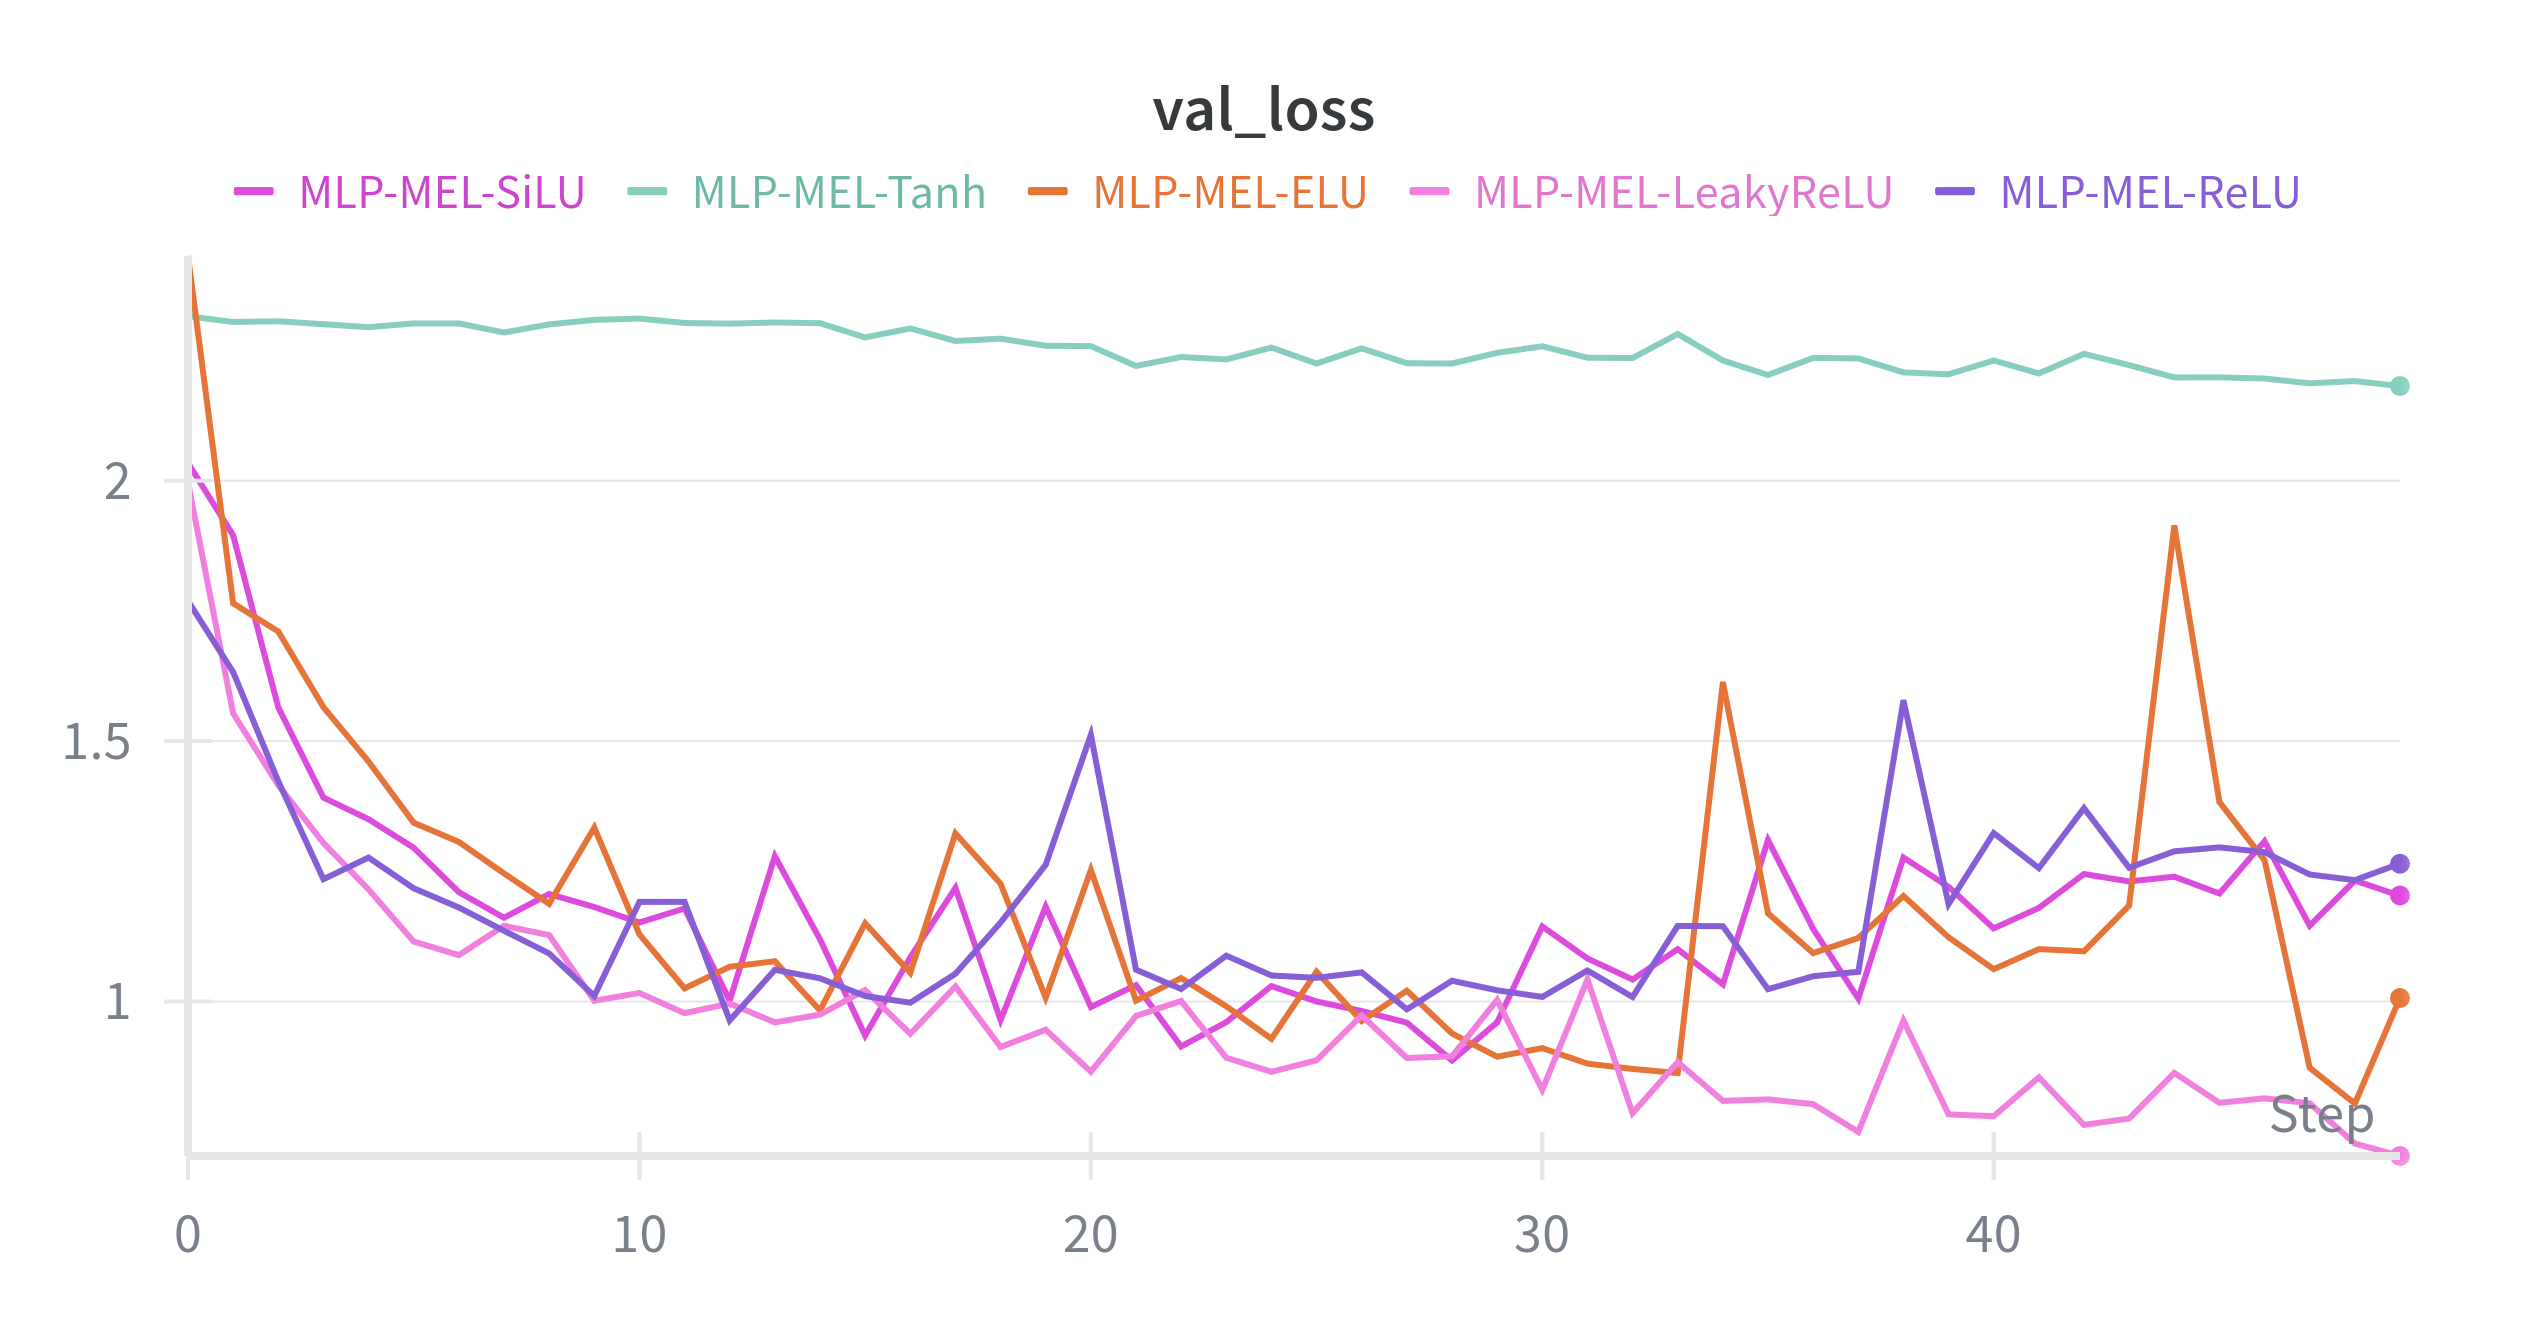
\includegraphics[width=\linewidth]{figs/4-val_loss.png}
    \caption{Validación — Loss}
  \end{subfigure}\hfill
  \begin{subfigure}{0.48\textwidth}\centering
    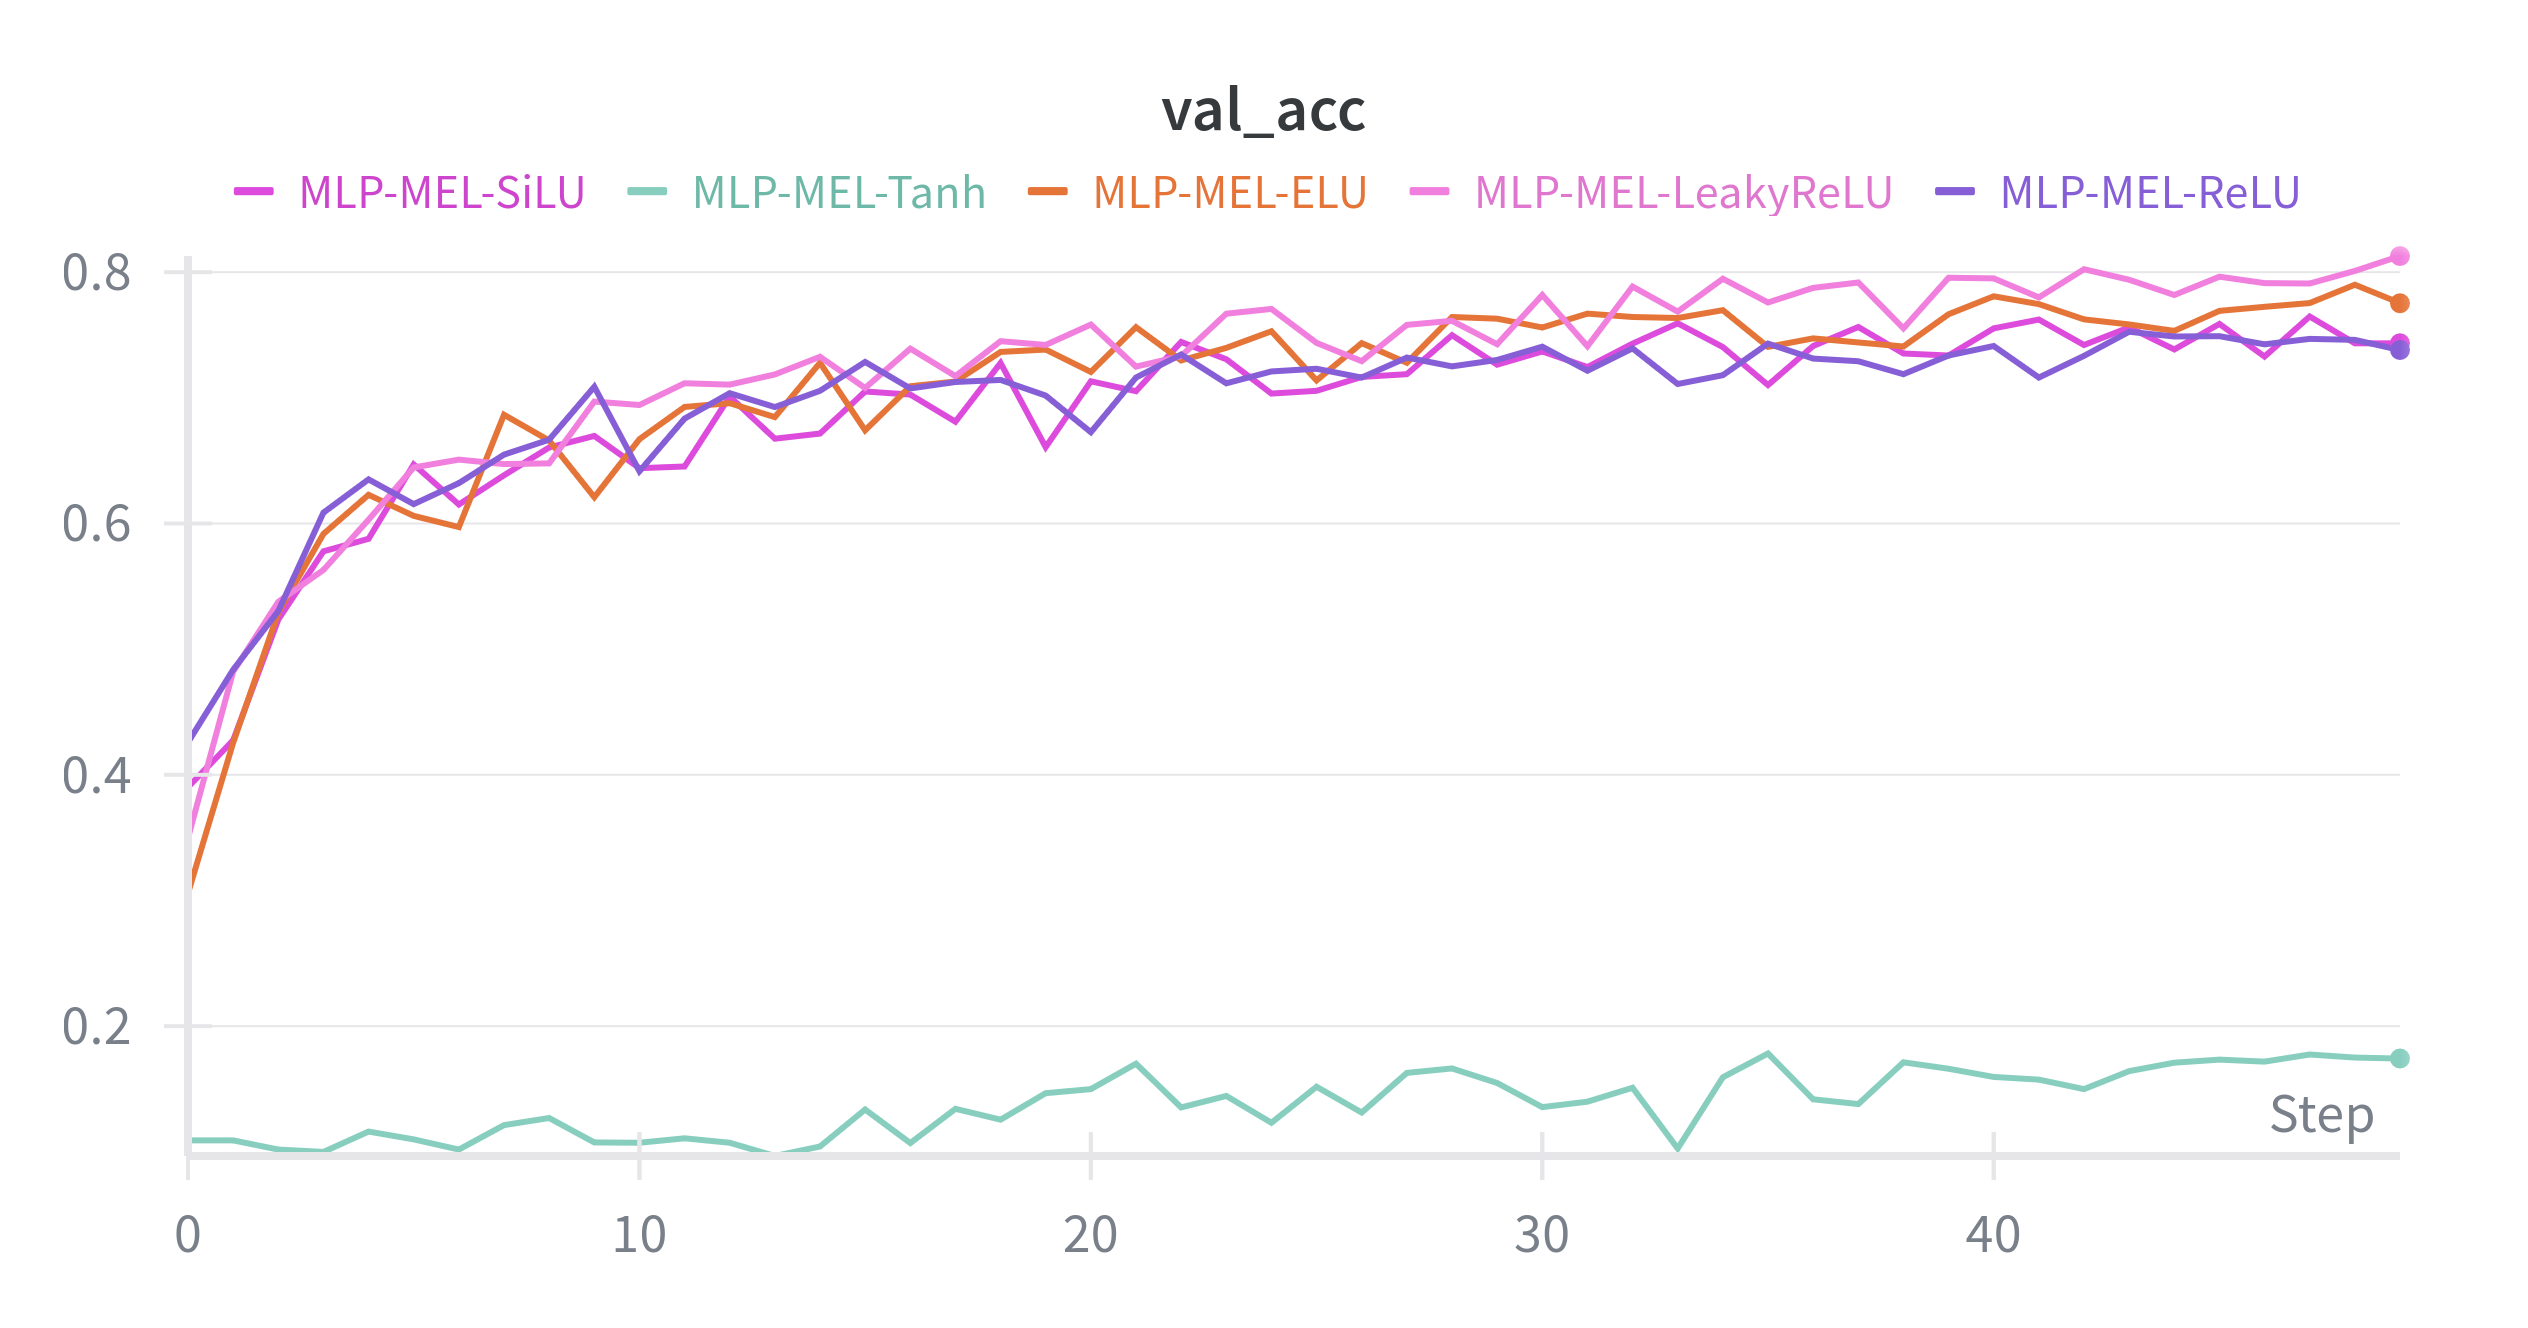
\includegraphics[width=\linewidth]{figs/4-val_acc.png}
    \caption{Validación — Accuracy}
  \end{subfigure}
  \caption{Comparativa de activaciones (Ej.4).}
\end{figure}

\noindent\textbf{Min/Max (W\&B).} ReLU/LeakyReLU: \texttt{val\_acc} hasta \(\approx 0.84\), \texttt{val\_loss} mínimo \(\approx 0.6\). \texttt{Tanh/Sigmoid}: \texttt{val\_acc} \(\approx 0.70\)–\(0.78\), \texttt{val\_loss} \(\approx 0.8\)–\(1.0\).\\
\textbf{Lectura.} Activaciones no saturantes (ReLU, Leaky) favorecen gradientes sanos y convergencia estable; Tanh muestra \emph{vanishing}.

\subsection*{Conclusión}
Las variantes basadas en ReLU convergieron más rápido y alcanzaron mejores métricas de validación. Tanh/Sigmoid mostraron mayores \texttt{val\_loss} y \texttt{val\_acc} inferiores, consistentes con saturación de gradientes.

% ==============================================================
\section*{Ejercicio 5 — Optimizadores}
\subsection*{Desarrollo}
\noindent
Se evaluaron SGD (con momentum), Adam y RMSprop, con y sin \textit{schedulers} de \texttt{lr}. Adam suele ofrecer buen compromiso entre velocidad y estabilidad; SGD puede igualarlo con ajuste fino y mayor número de épocas.

\subsection*{Resultados (curvas)}
\begin{figure}[H]\centering
  \begin{subfigure}{0.48\textwidth}\centering
    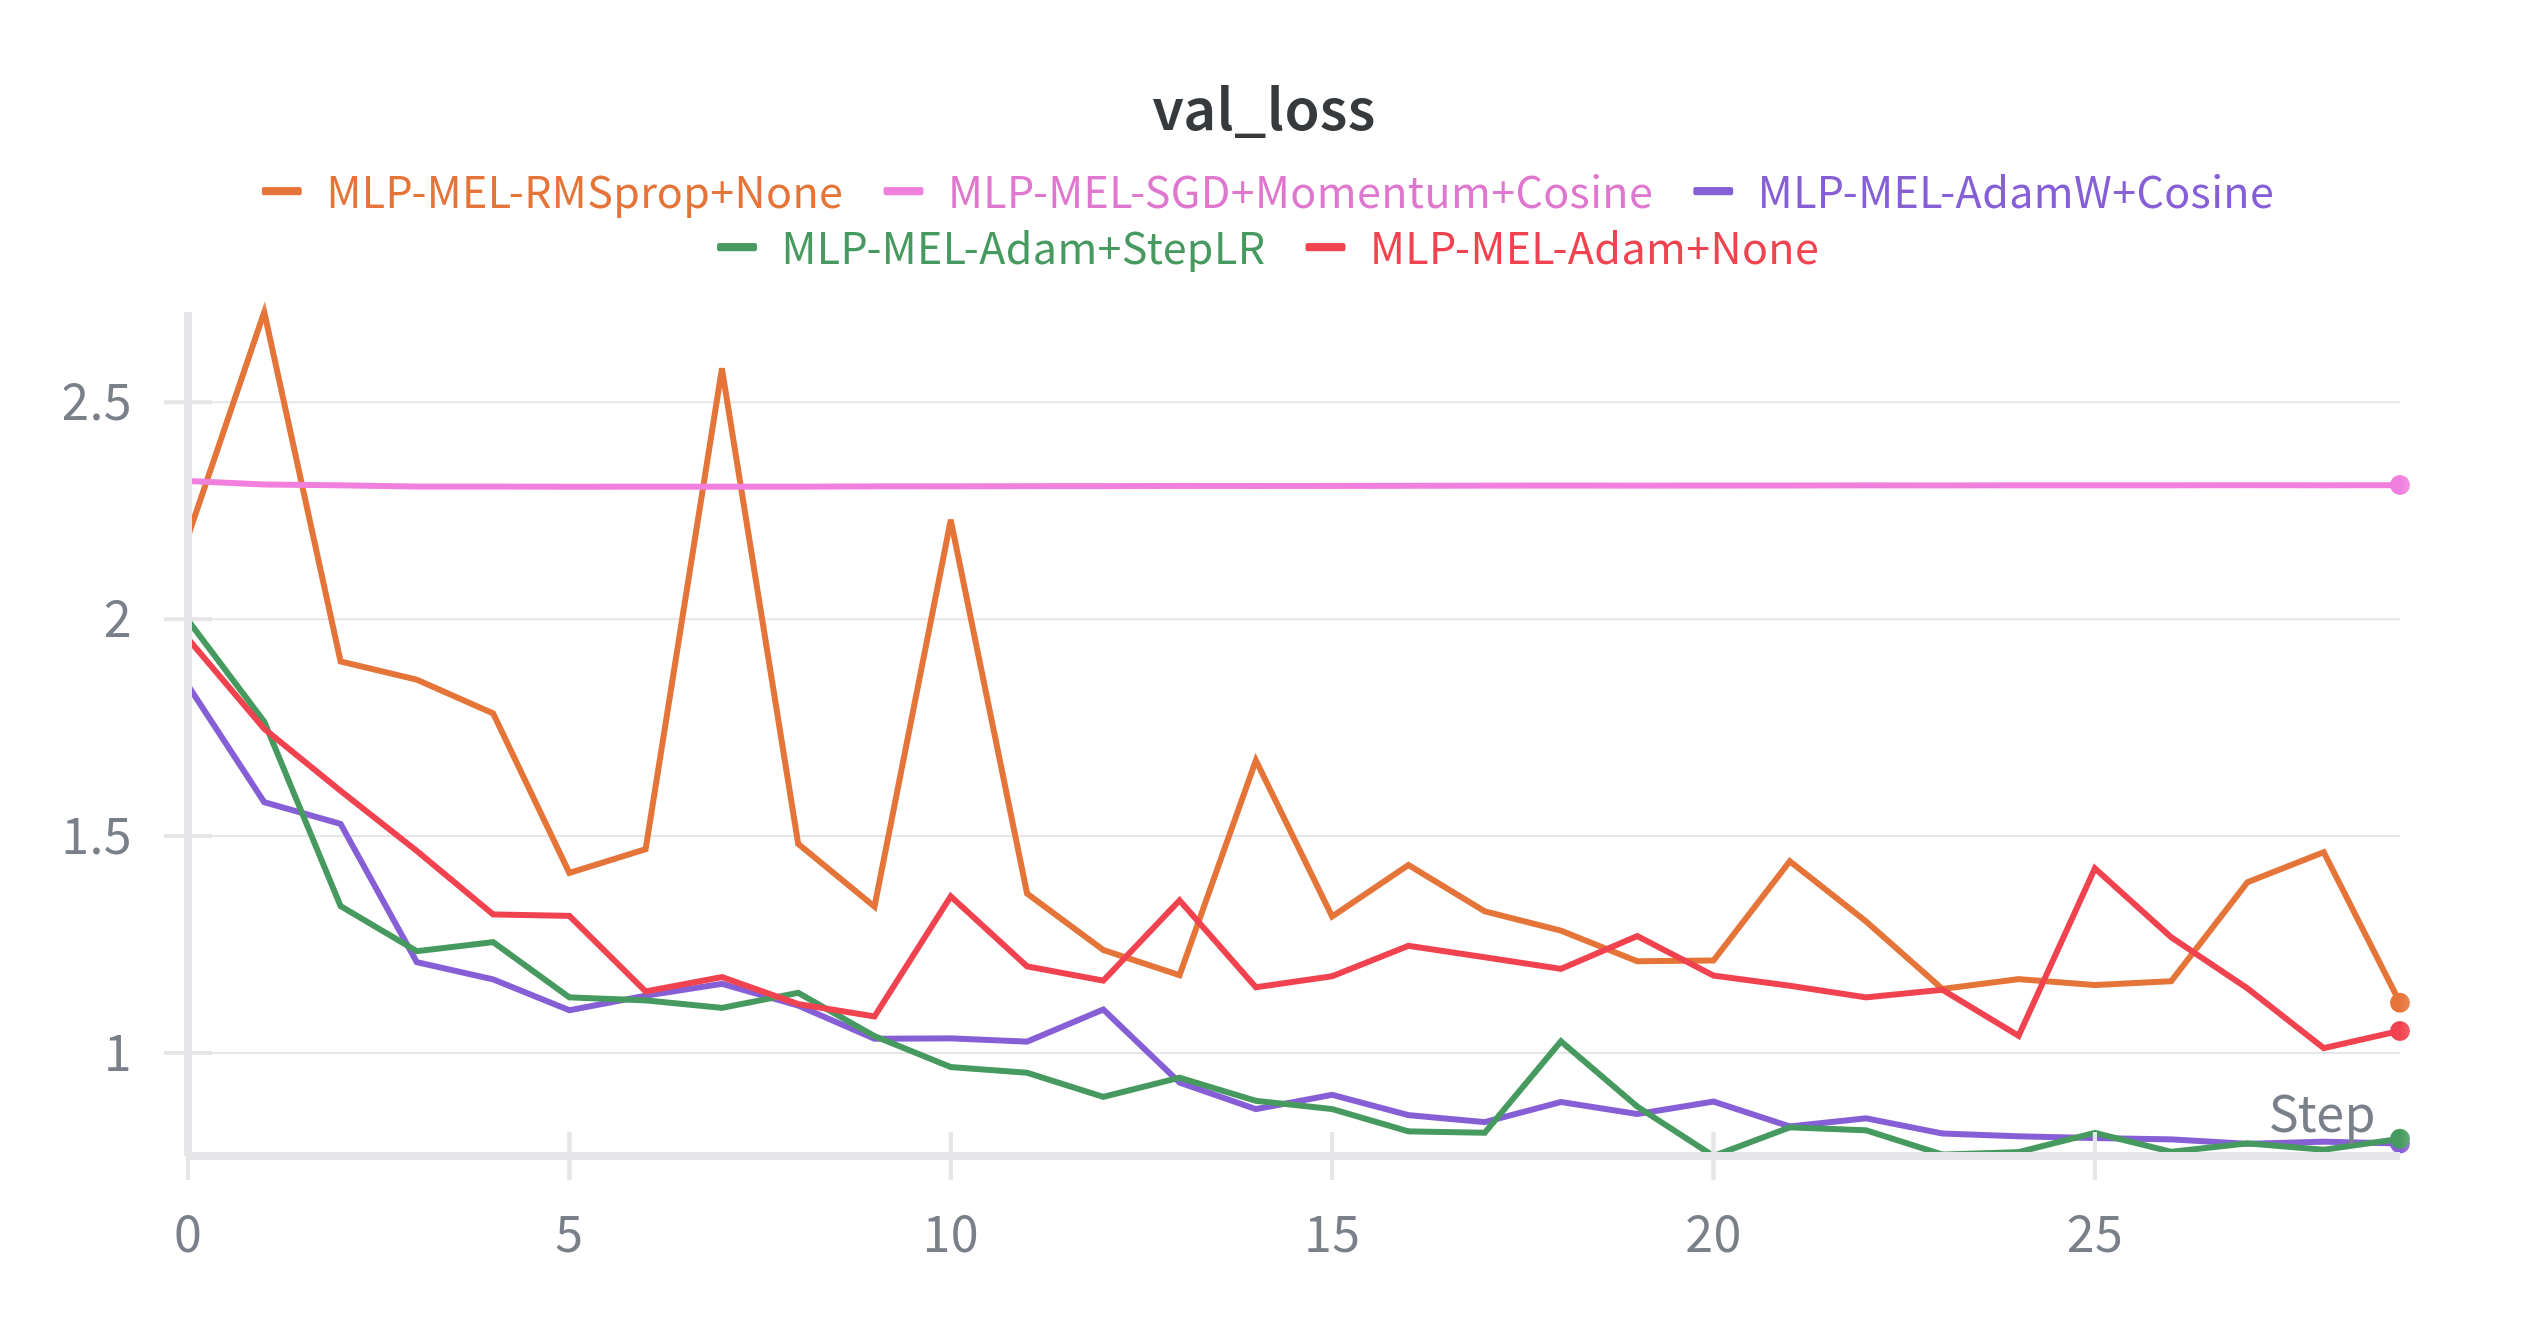
\includegraphics[width=\linewidth]{figs/5-val_loss.png}
    \caption{Validación — Loss}
  \end{subfigure}\hfill
  \begin{subfigure}{0.48\textwidth}\centering
    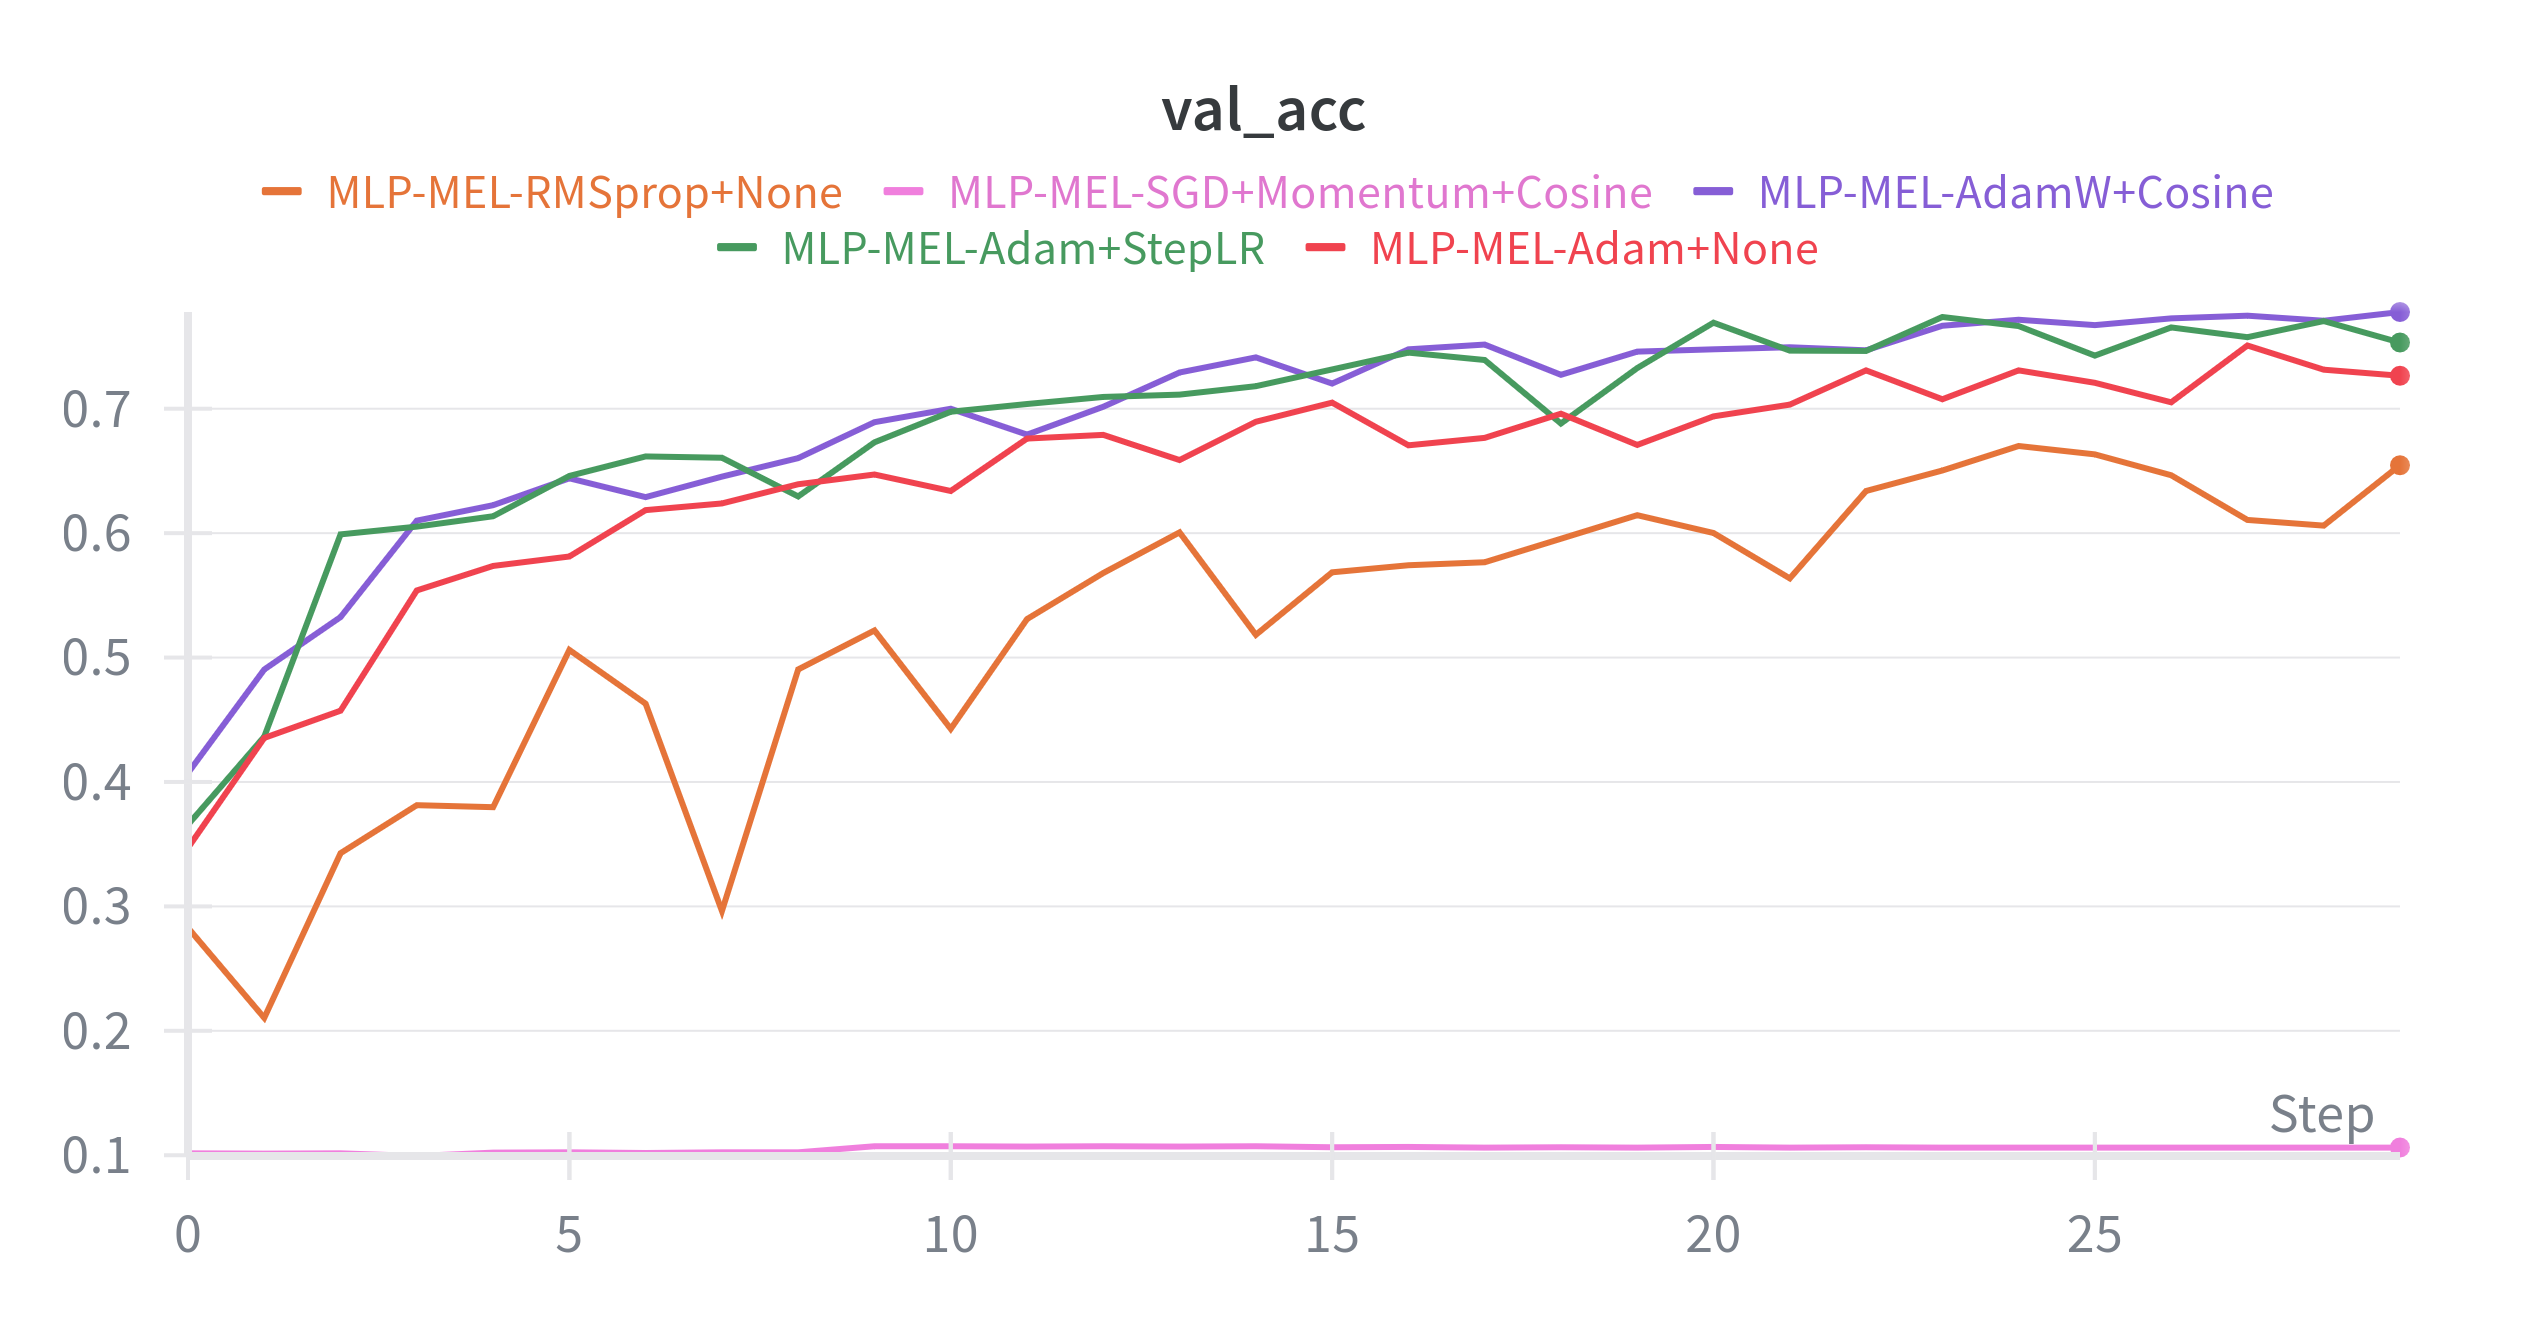
\includegraphics[width=\linewidth]{figs/5-val_acc.png}
    \caption{Validación — Accuracy}
  \end{subfigure}
  \caption{Comparativa de optimizadores (Ej.5).}
\end{figure}

\noindent\textbf{Min/Max (W\&B).} \texttt{Adam/AdamW}: \textit{val\_acc} hasta \(\approx 0.87\), \textit{val\_loss} mínimo \(\approx 0.6\). \texttt{SGD}: \textit{val\_acc} típica \(\approx 0.75\)–\(0.80\), \textit{val\_loss} \(\approx 0.8\)–\(1.0\).\\
\textbf{Lectura.} \texttt{AdamW} domina en velocidad y estabilidad; \texttt{StepLR} mitiga mesetas.

\subsection*{Conclusión}
Adam logró menor \texttt{val\_loss} y mayor \texttt{val\_acc} en menos épocas; SGD con momentum se aproximó con más tiempo de entrenamiento. RMSprop quedó intermedio.

% ==============================================================
\section*{Ejercicio 6 — Arquitectura CNN}
\subsection*{Desarrollo}
\noindent
Diseñamos una CNN pequeña–mediana (3 bloques \texttt{Conv2D–BN–ReLU–MaxPool} y \texttt{Linear} final). Se exploró agregar \texttt{Dropout} y \texttt{Weight Decay}, manteniendo \texttt{Adam} y \texttt{CrossEntropyLoss}. En CNNs sobre MEL, el sesgo inductivo capta patrones locales (formantes, transiciones) de manera robusta.

\subsection*{Resultados (curvas)}
\begin{figure}[H]\centering
  \begin{subfigure}{0.48\textwidth}\centering
    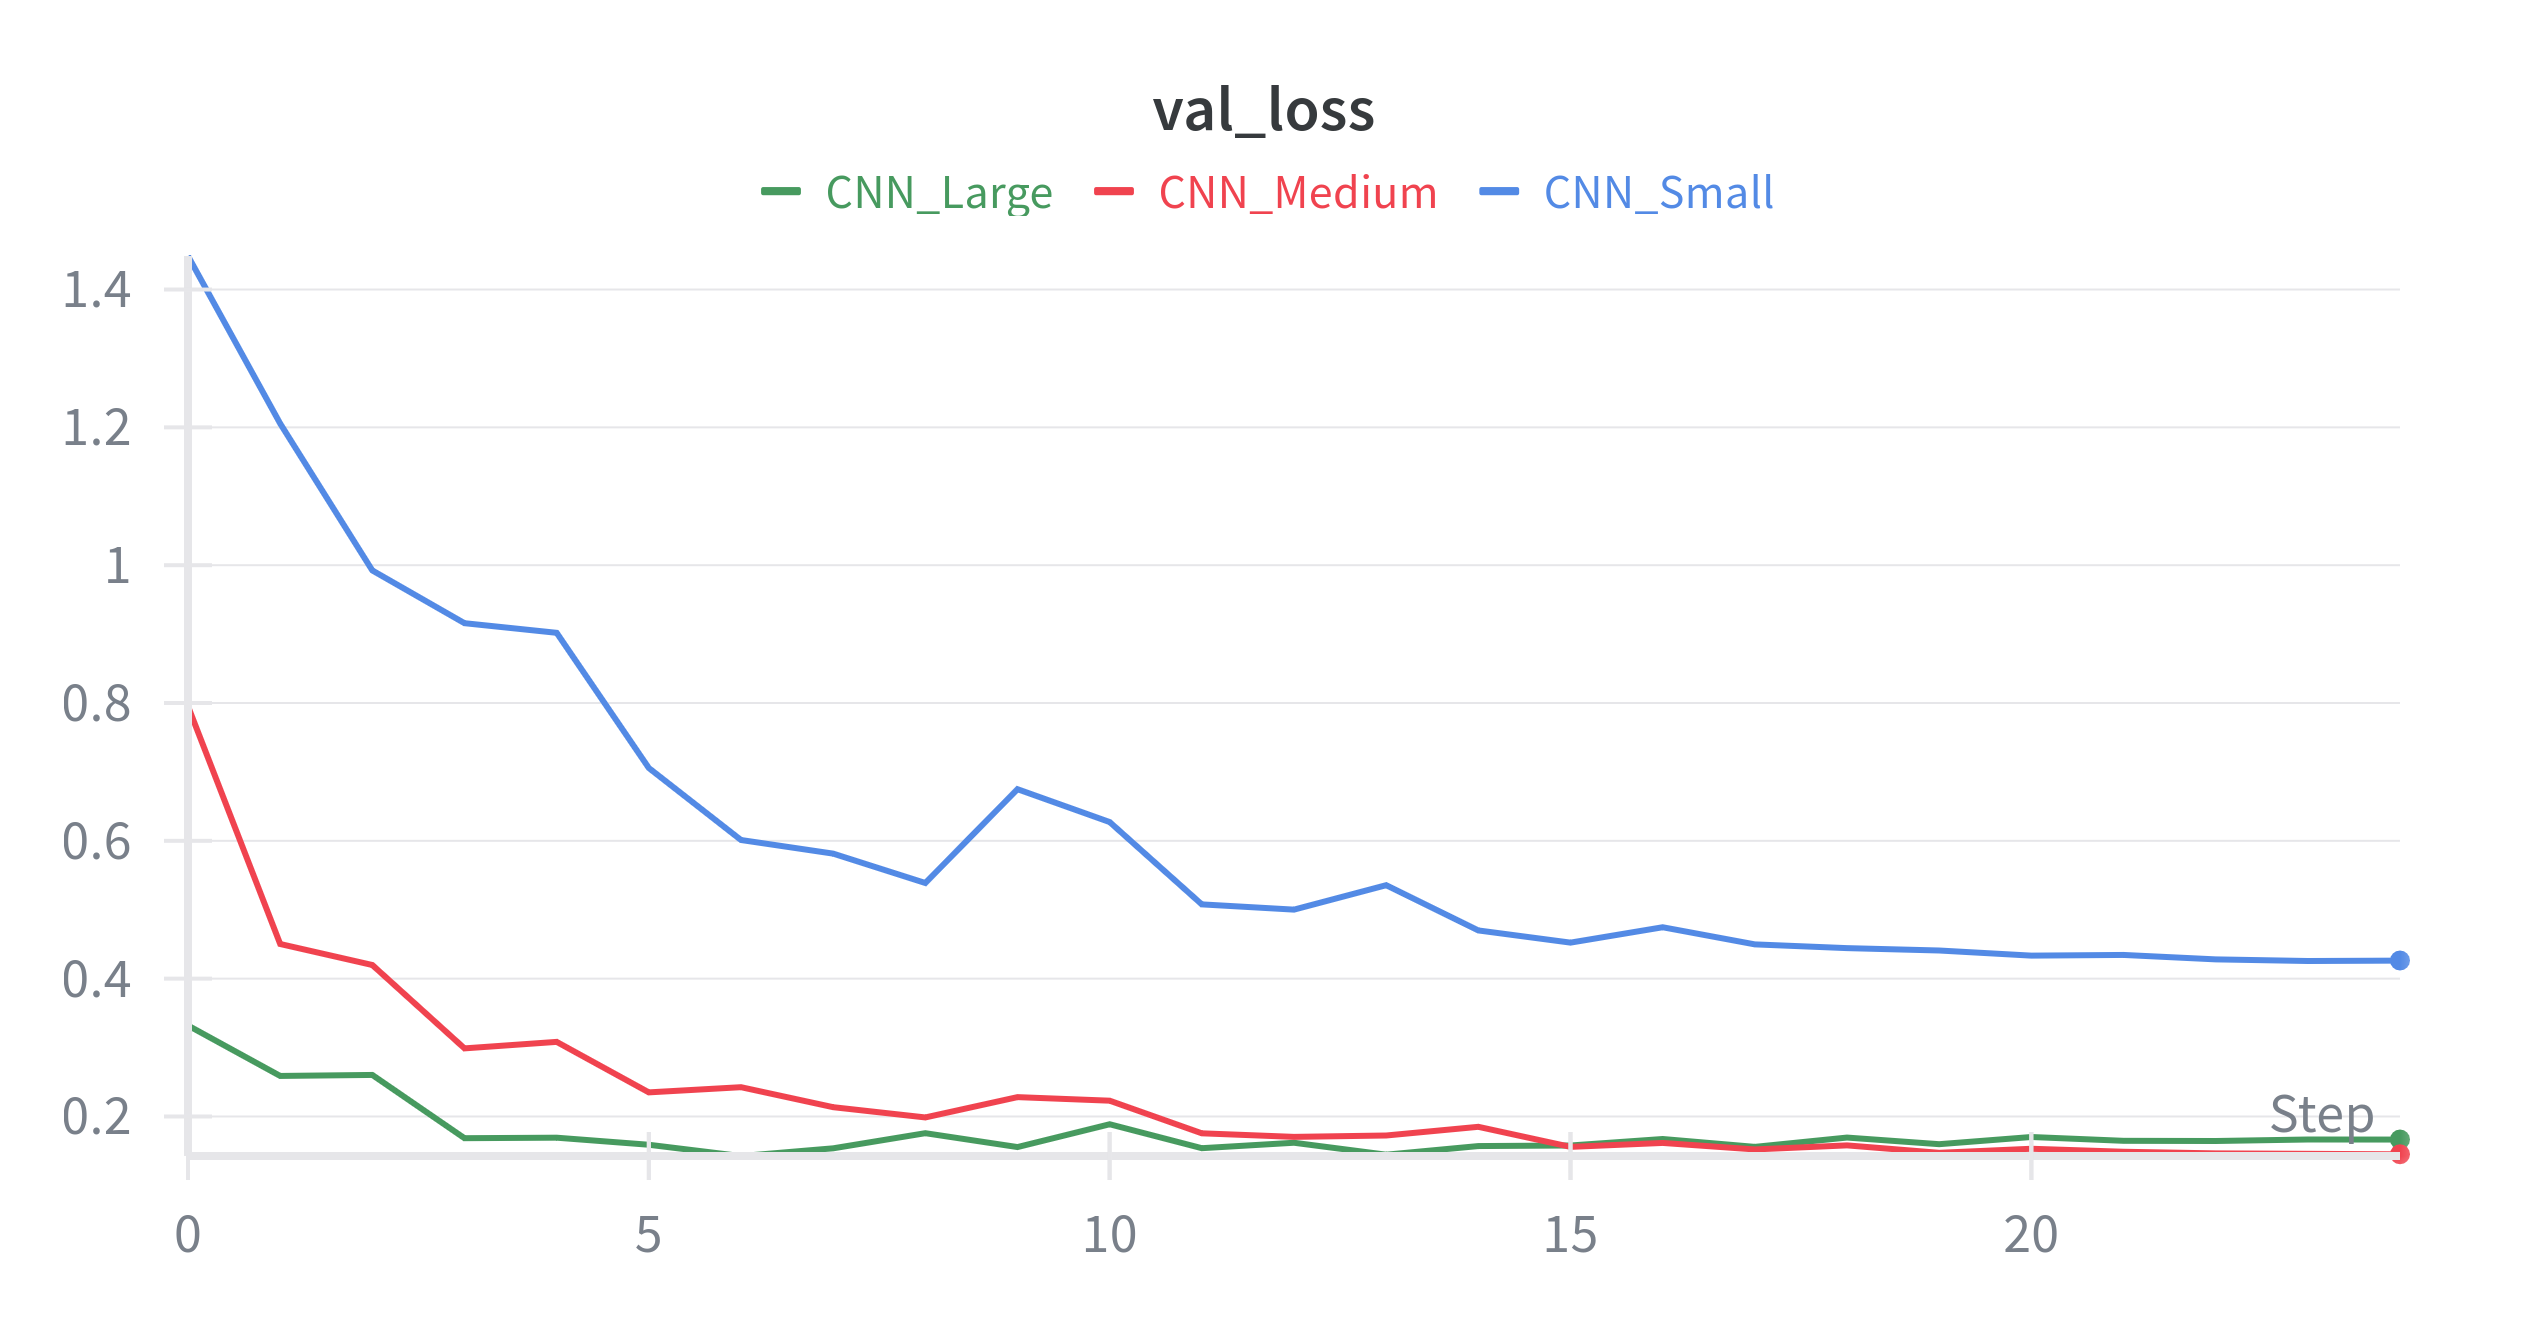
\includegraphics[width=\linewidth]{figs/6-val_loss.png}
    \caption{Validación — Loss}
  \end{subfigure}\hfill
  \begin{subfigure}{0.48\textwidth}\centering
    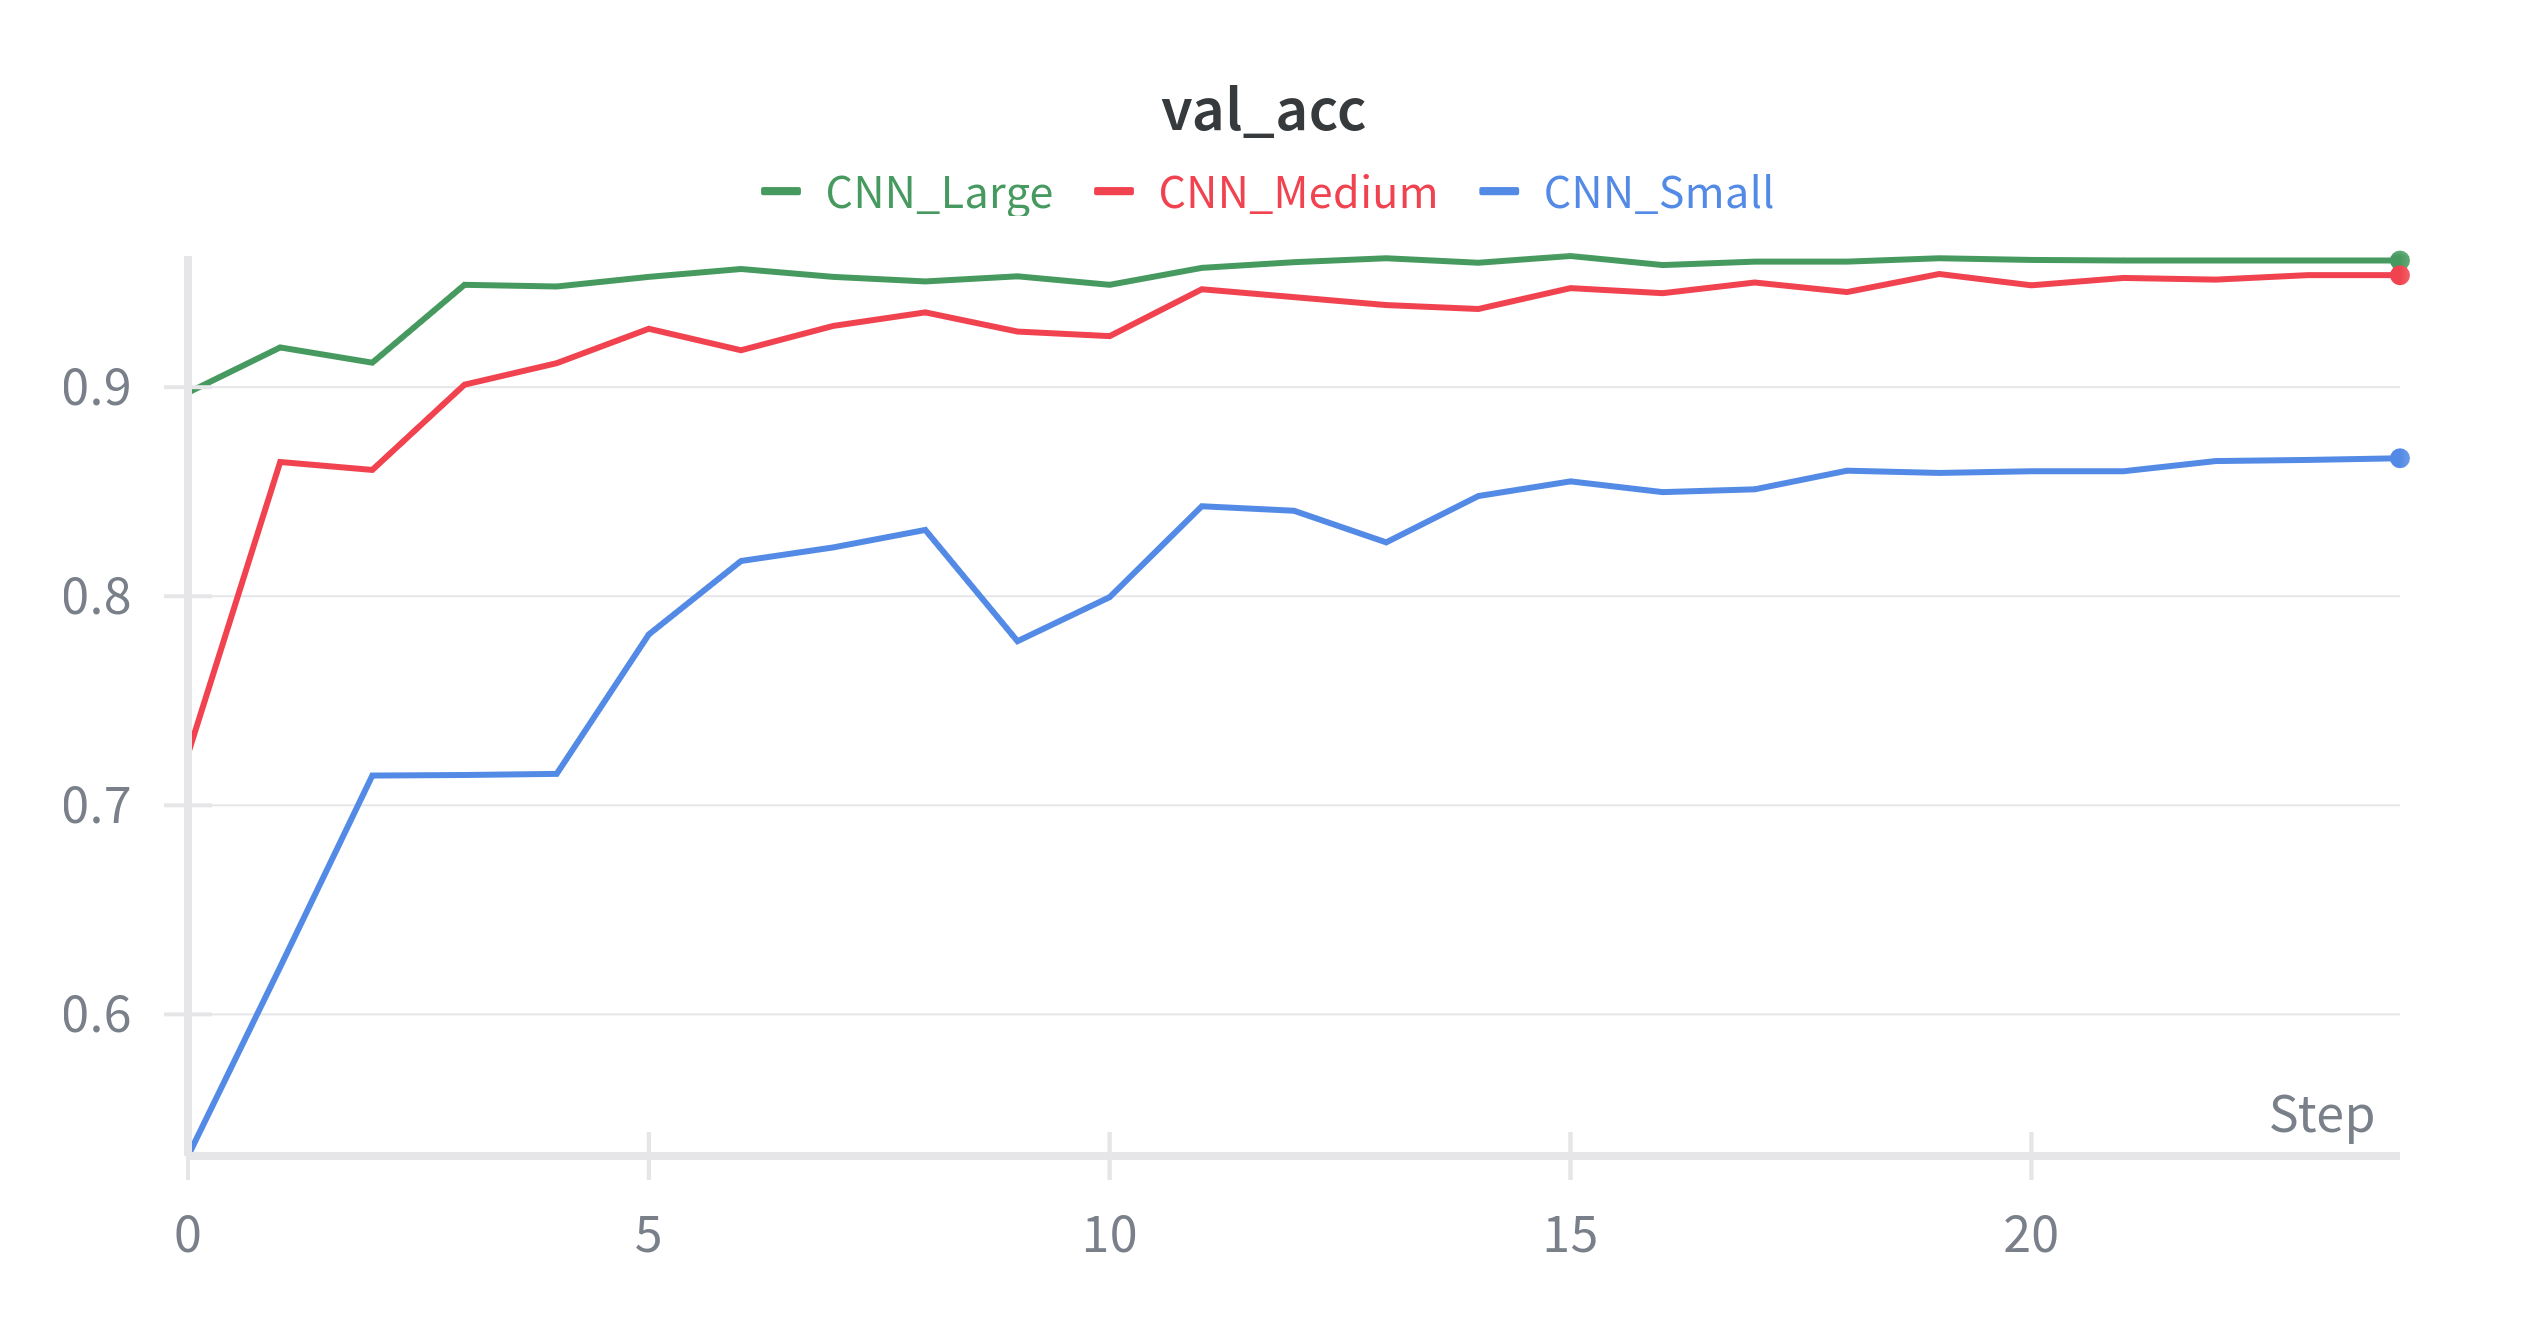
\includegraphics[width=\linewidth]{figs/6-val_acc.png}
    \caption{Validación — Accuracy}
  \end{subfigure}
  \caption{Variantes de CNN (Ej.6).}
\end{figure}

\noindent\textbf{Min/Max (W\&B).} \texttt{val\_acc} \(\approx 0.92\)–\(0.95\); \texttt{val\_loss} \(\approx 0.18\)–\(0.30\).\\
\textbf{Lectura.} Convergencia rápida y estable; regularización ligera mejora suavidad de curvas sin perder accuracy.

\subsection*{Conclusión}
\noindent La CNN mediana con regularización ligera alcanzó la mejor \texttt{val\_acc} (\(\approx 0.95\)) con \texttt{val\_loss} baja y curvas estables, superando consistentemente a MLP.

% ==============================================================
\section*{Ejercicio 7 — Entrenamiento (batch size / épocas)}
\subsection*{Desarrollo}
\noindent
Se variaron \texttt{BATCH\_SIZE} (32, 64, 128) y \texttt{EPOCHS} (15, 25, 50). Teóricamente, los \textit{batches} grandes reducen el ruido del gradiente pero pueden empeorar la generalización; más épocas mejoran el ajuste pero incrementan el overfitting.

\subsection*{Resultados (curvas)}
\begin{figure}[H]\centering
  \begin{subfigure}{0.48\textwidth}\centering
    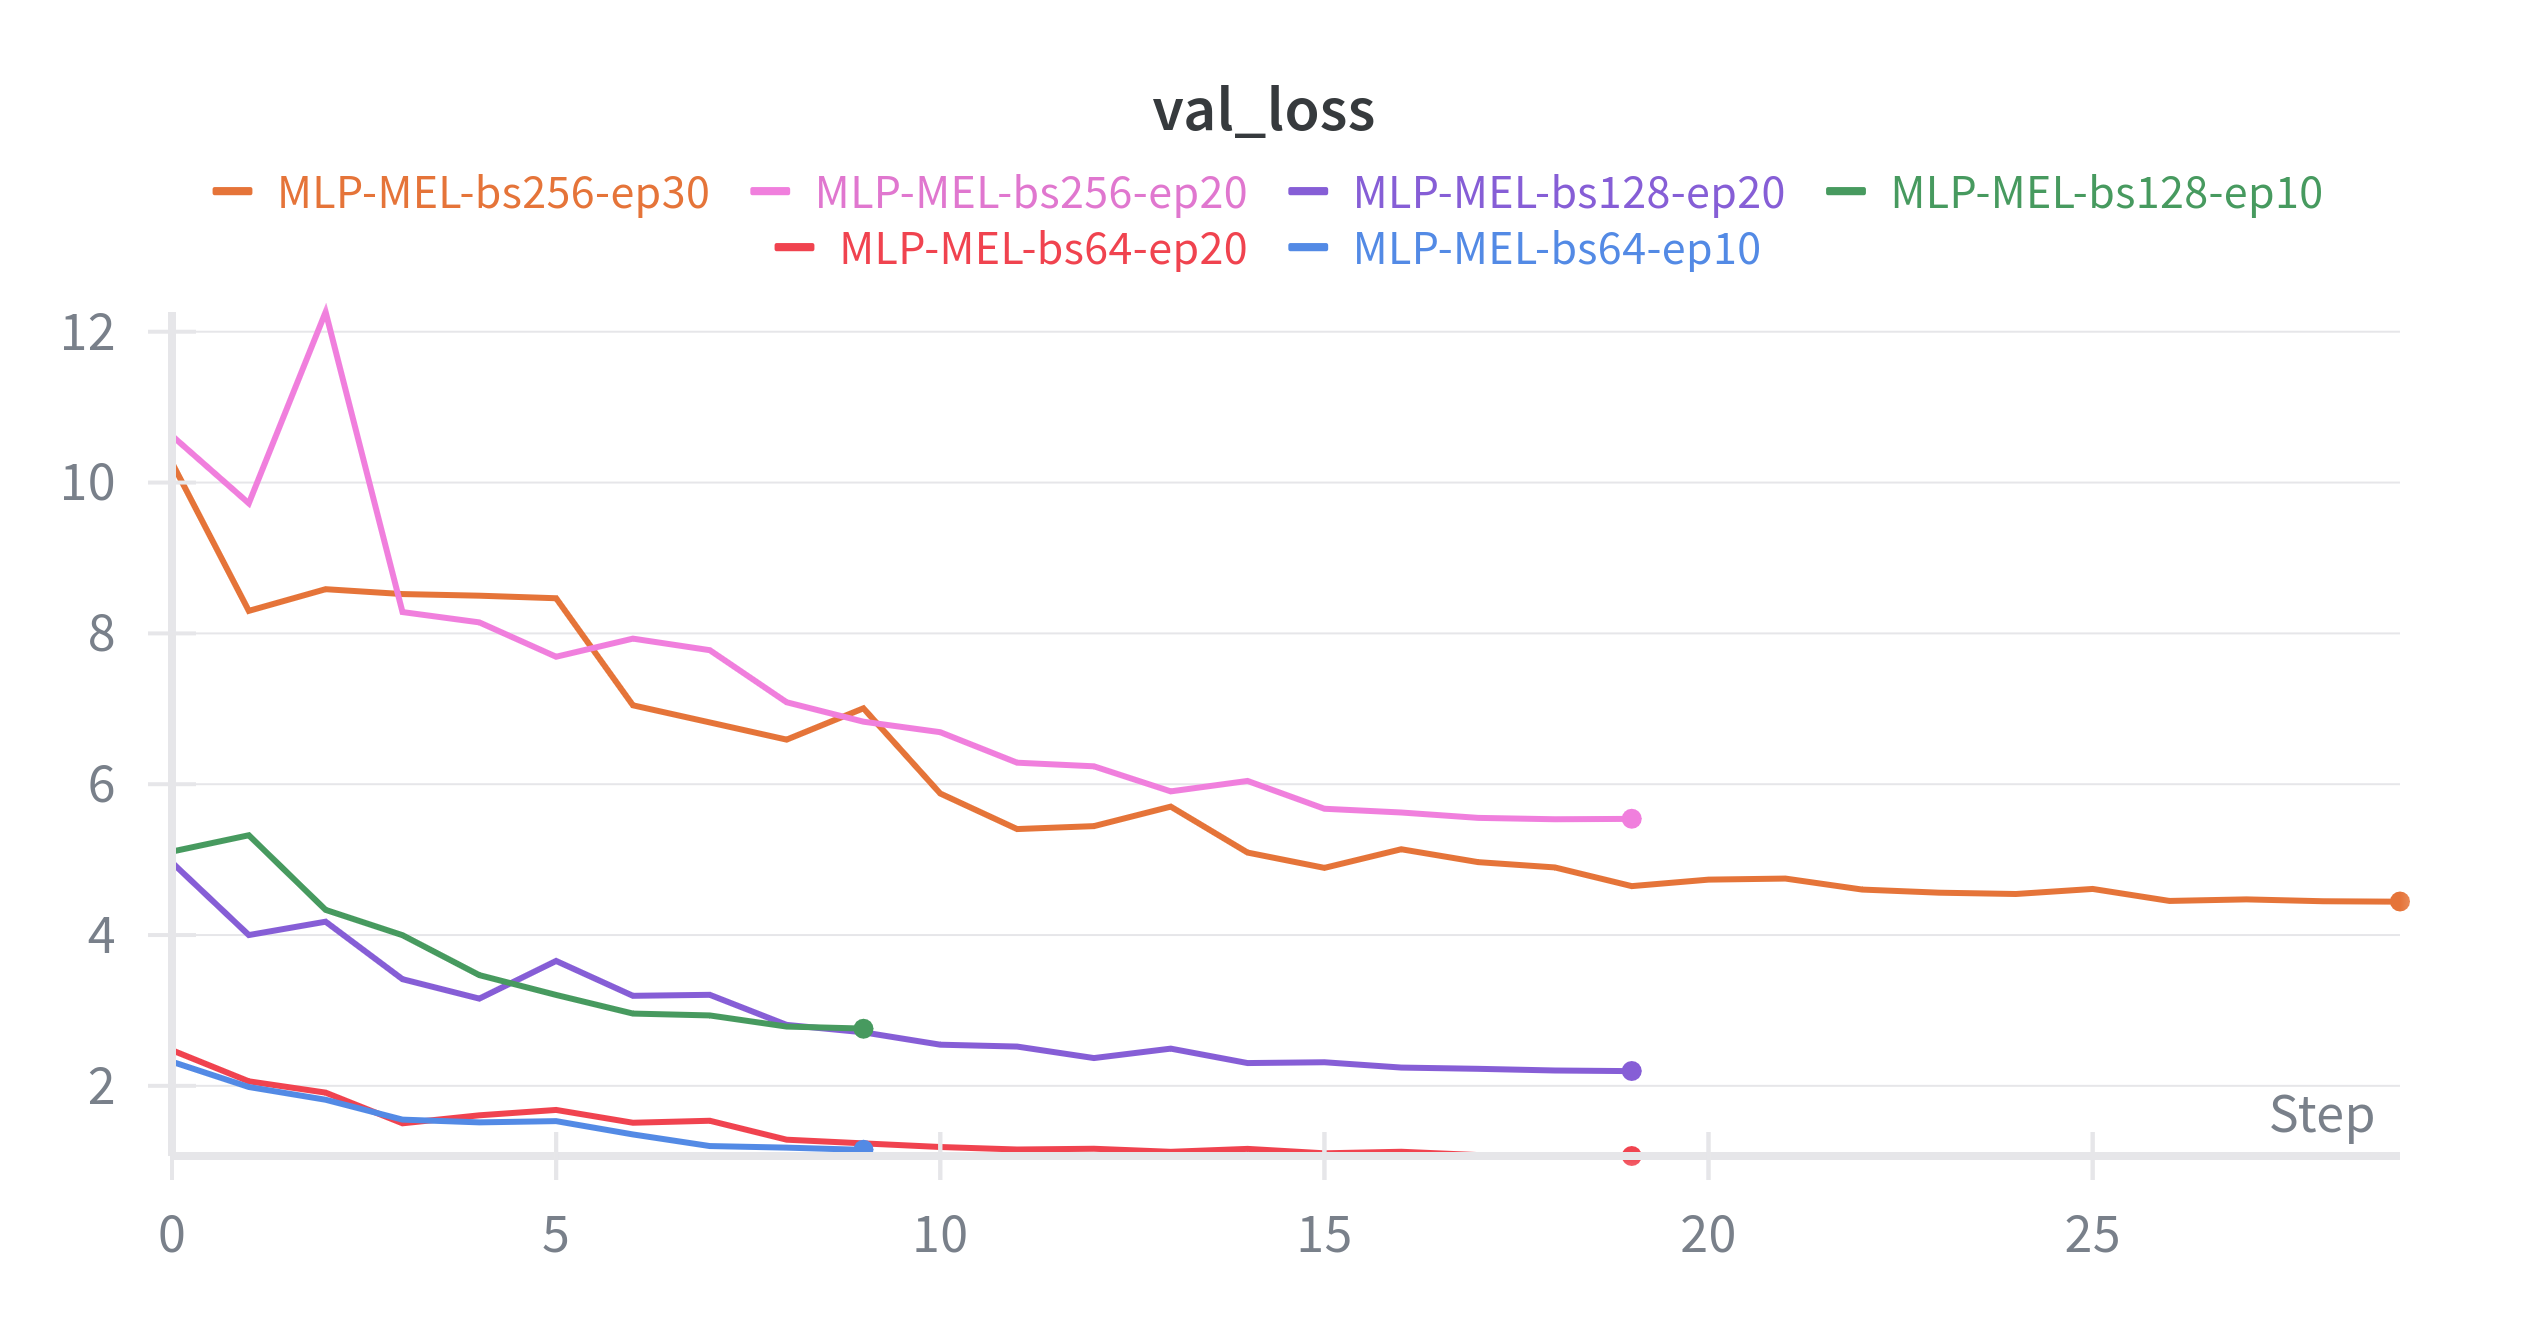
\includegraphics[width=\linewidth]{figs/7-val_loss.png}
    \caption{Validación — Loss (set 7)}
  \end{subfigure}\hfill
  \begin{subfigure}{0.48\textwidth}\centering
    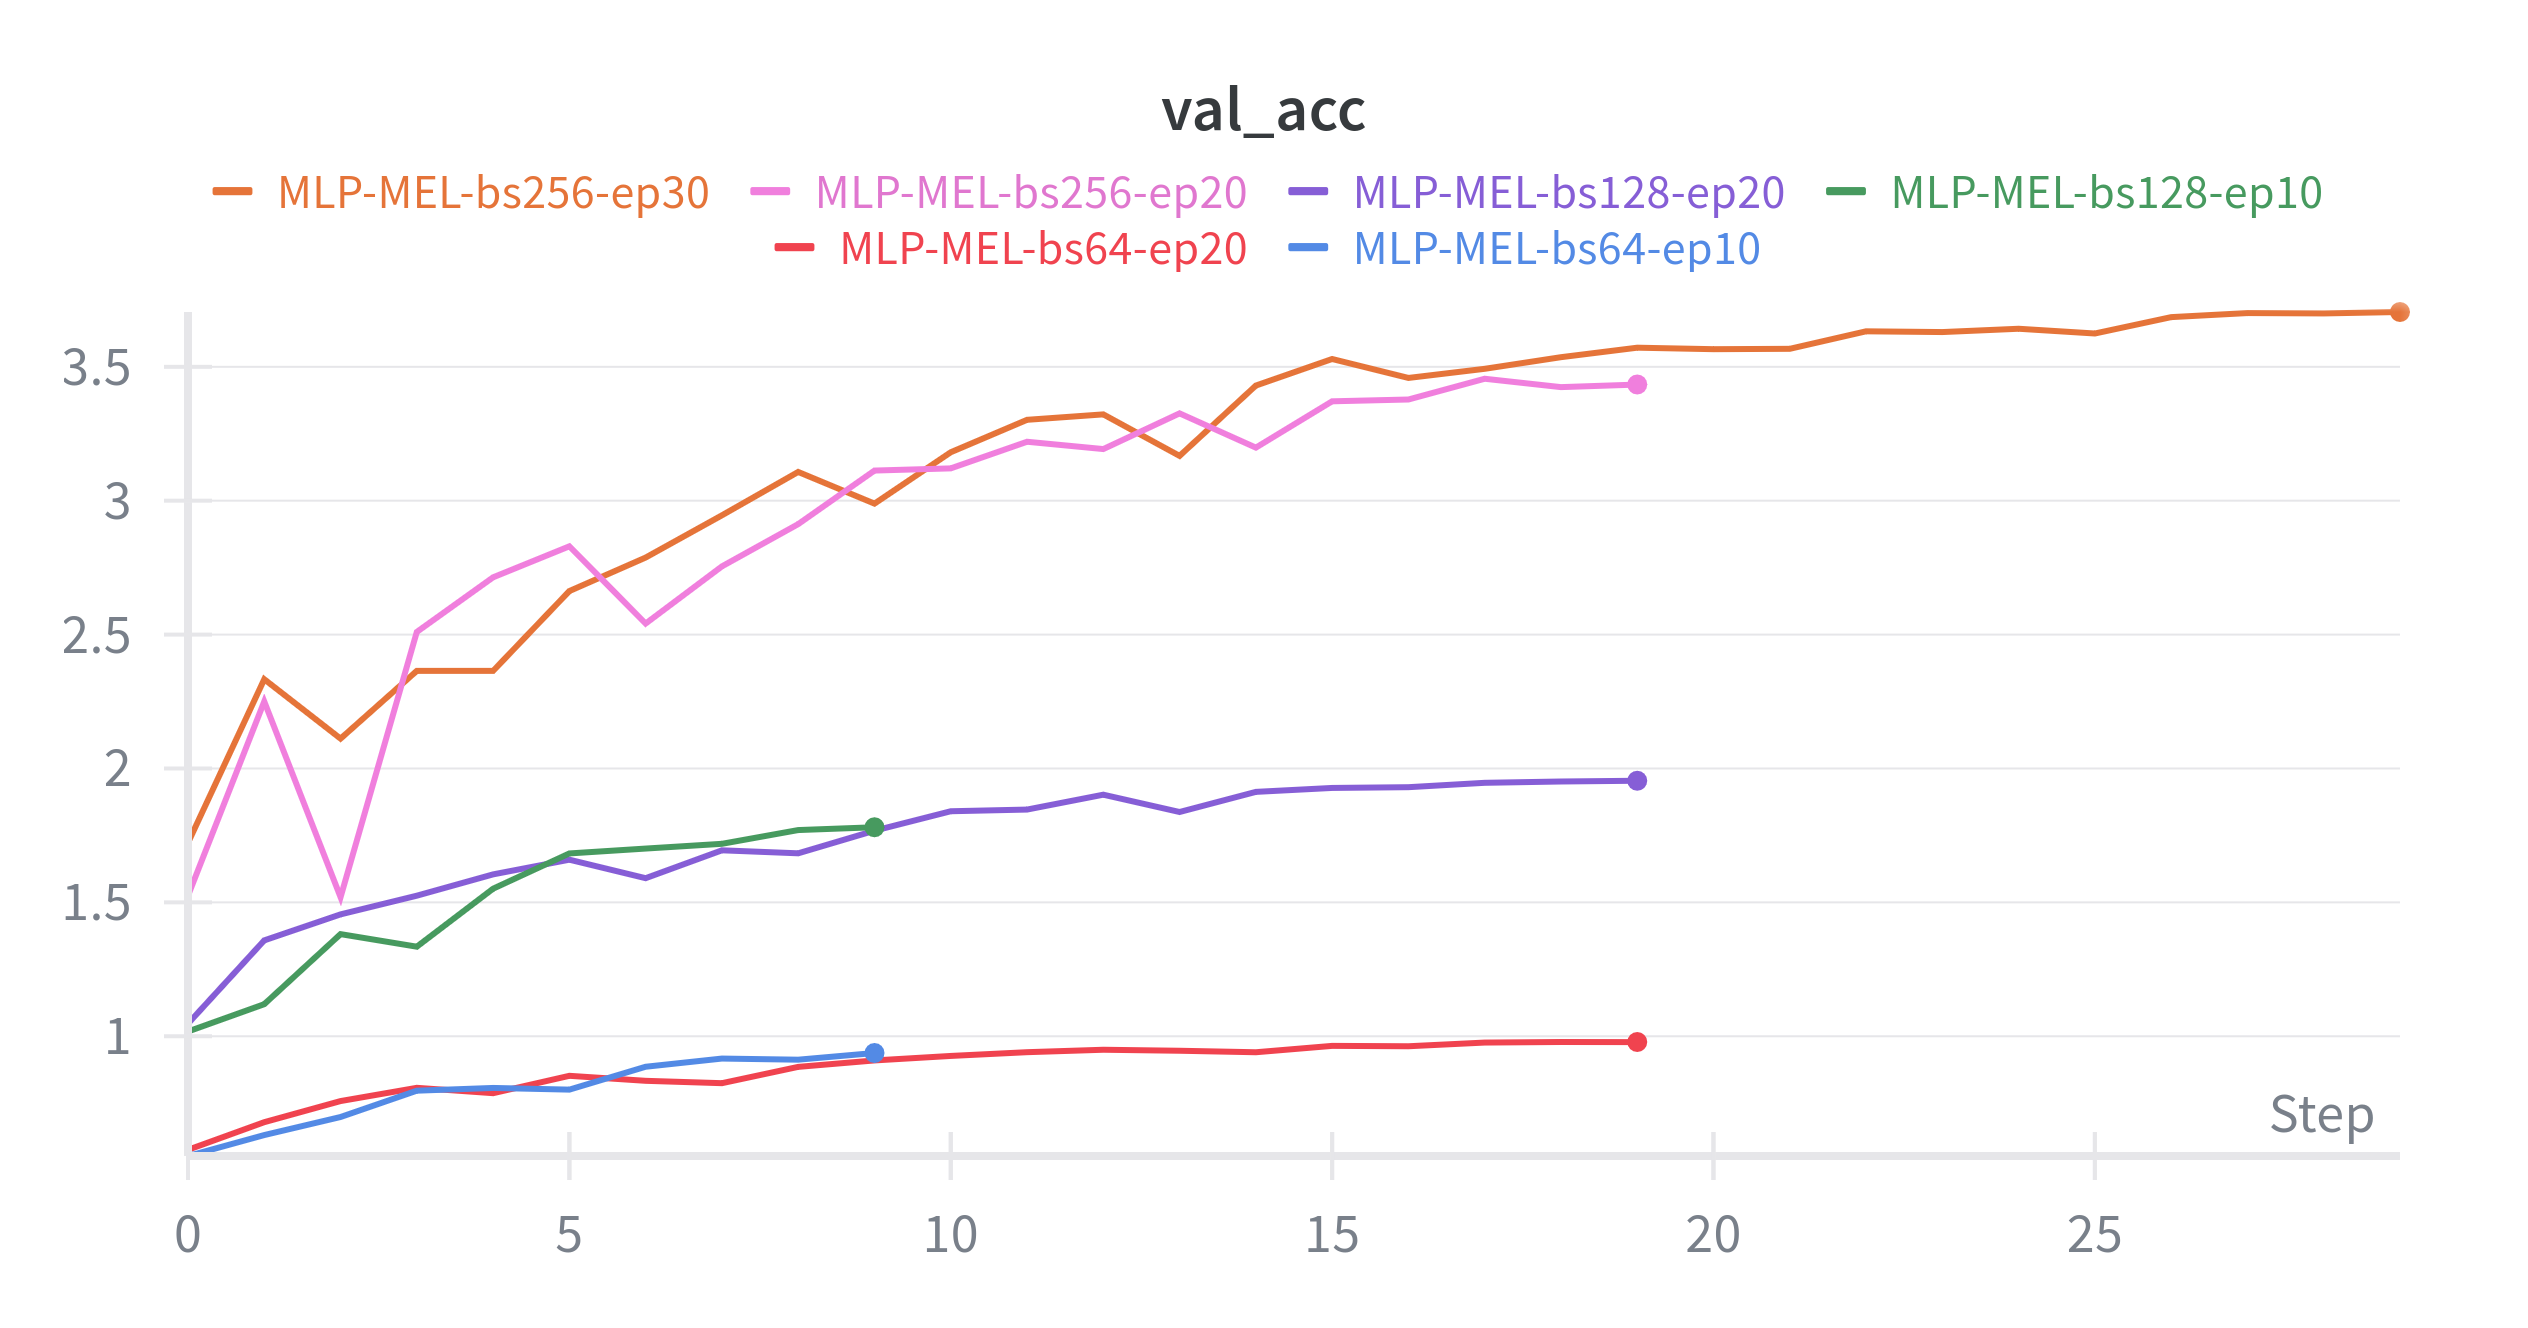
\includegraphics[width=\linewidth]{figs/7-val_acc.png}
    \caption{Validación — Accuracy (set 7)}
  \end{subfigure}
  \caption{Comparaciones de esquema de entrenamiento (Ej.7).}
\end{figure}

\noindent\textbf{Min/Max (W\&B).} \textbf{Mejor}: \texttt{BATCH\_SIZE} = 64, \texttt{val\_acc} $\approx$ 0.88 – 0.89, \texttt{val\_loss} mínima $\approx$ 0.5. \textbf{Peor}: \texttt{BATCH\_SIZE} > 64, \texttt{val\_acc} \(\approx 0.80\), \texttt{val\_loss} $\approx$ 0.85 – 0.90.\\
\textbf{Lectura.} Los batches pequeños generalizan mejor; extender épocas más allá de \(\sim 30\) rinde retornos decrecientes.

\begin{figure}[H]\centering
  \begin{subfigure}{0.48\textwidth}\centering
    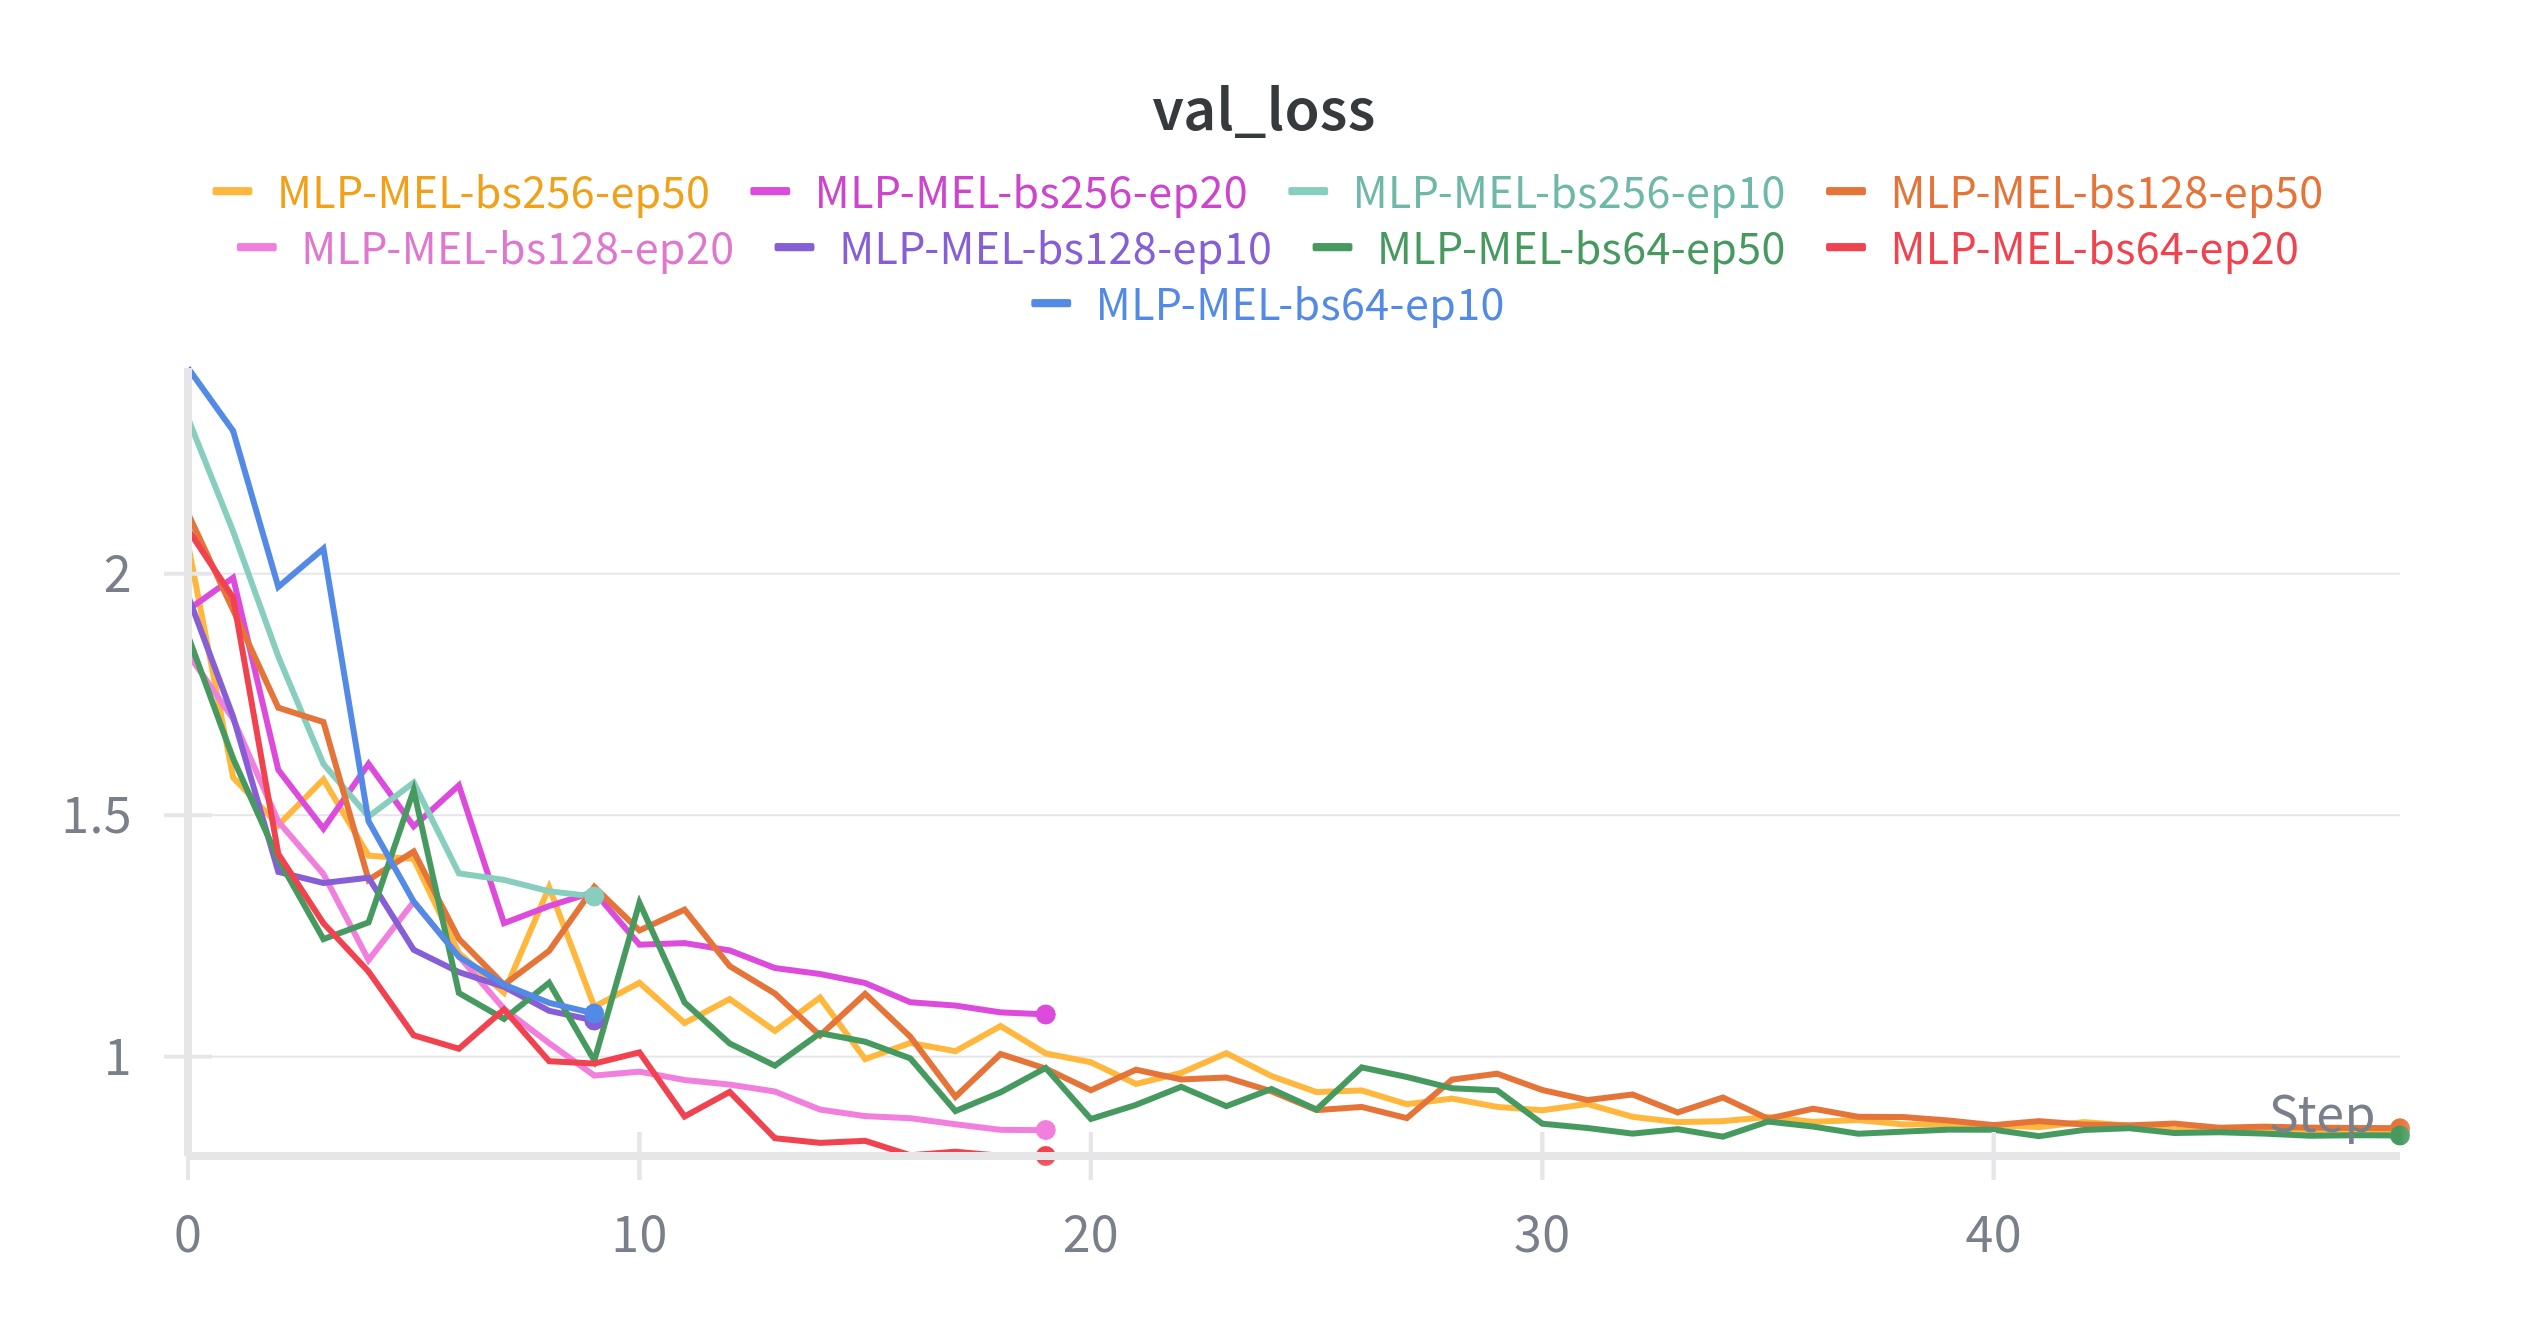
\includegraphics[width=\linewidth]{figs/7.2-val_loss.png}
    \caption{Validación — Loss (set 7.2)}
  \end{subfigure}\hfill
  \begin{subfigure}{0.48\textwidth}\centering
    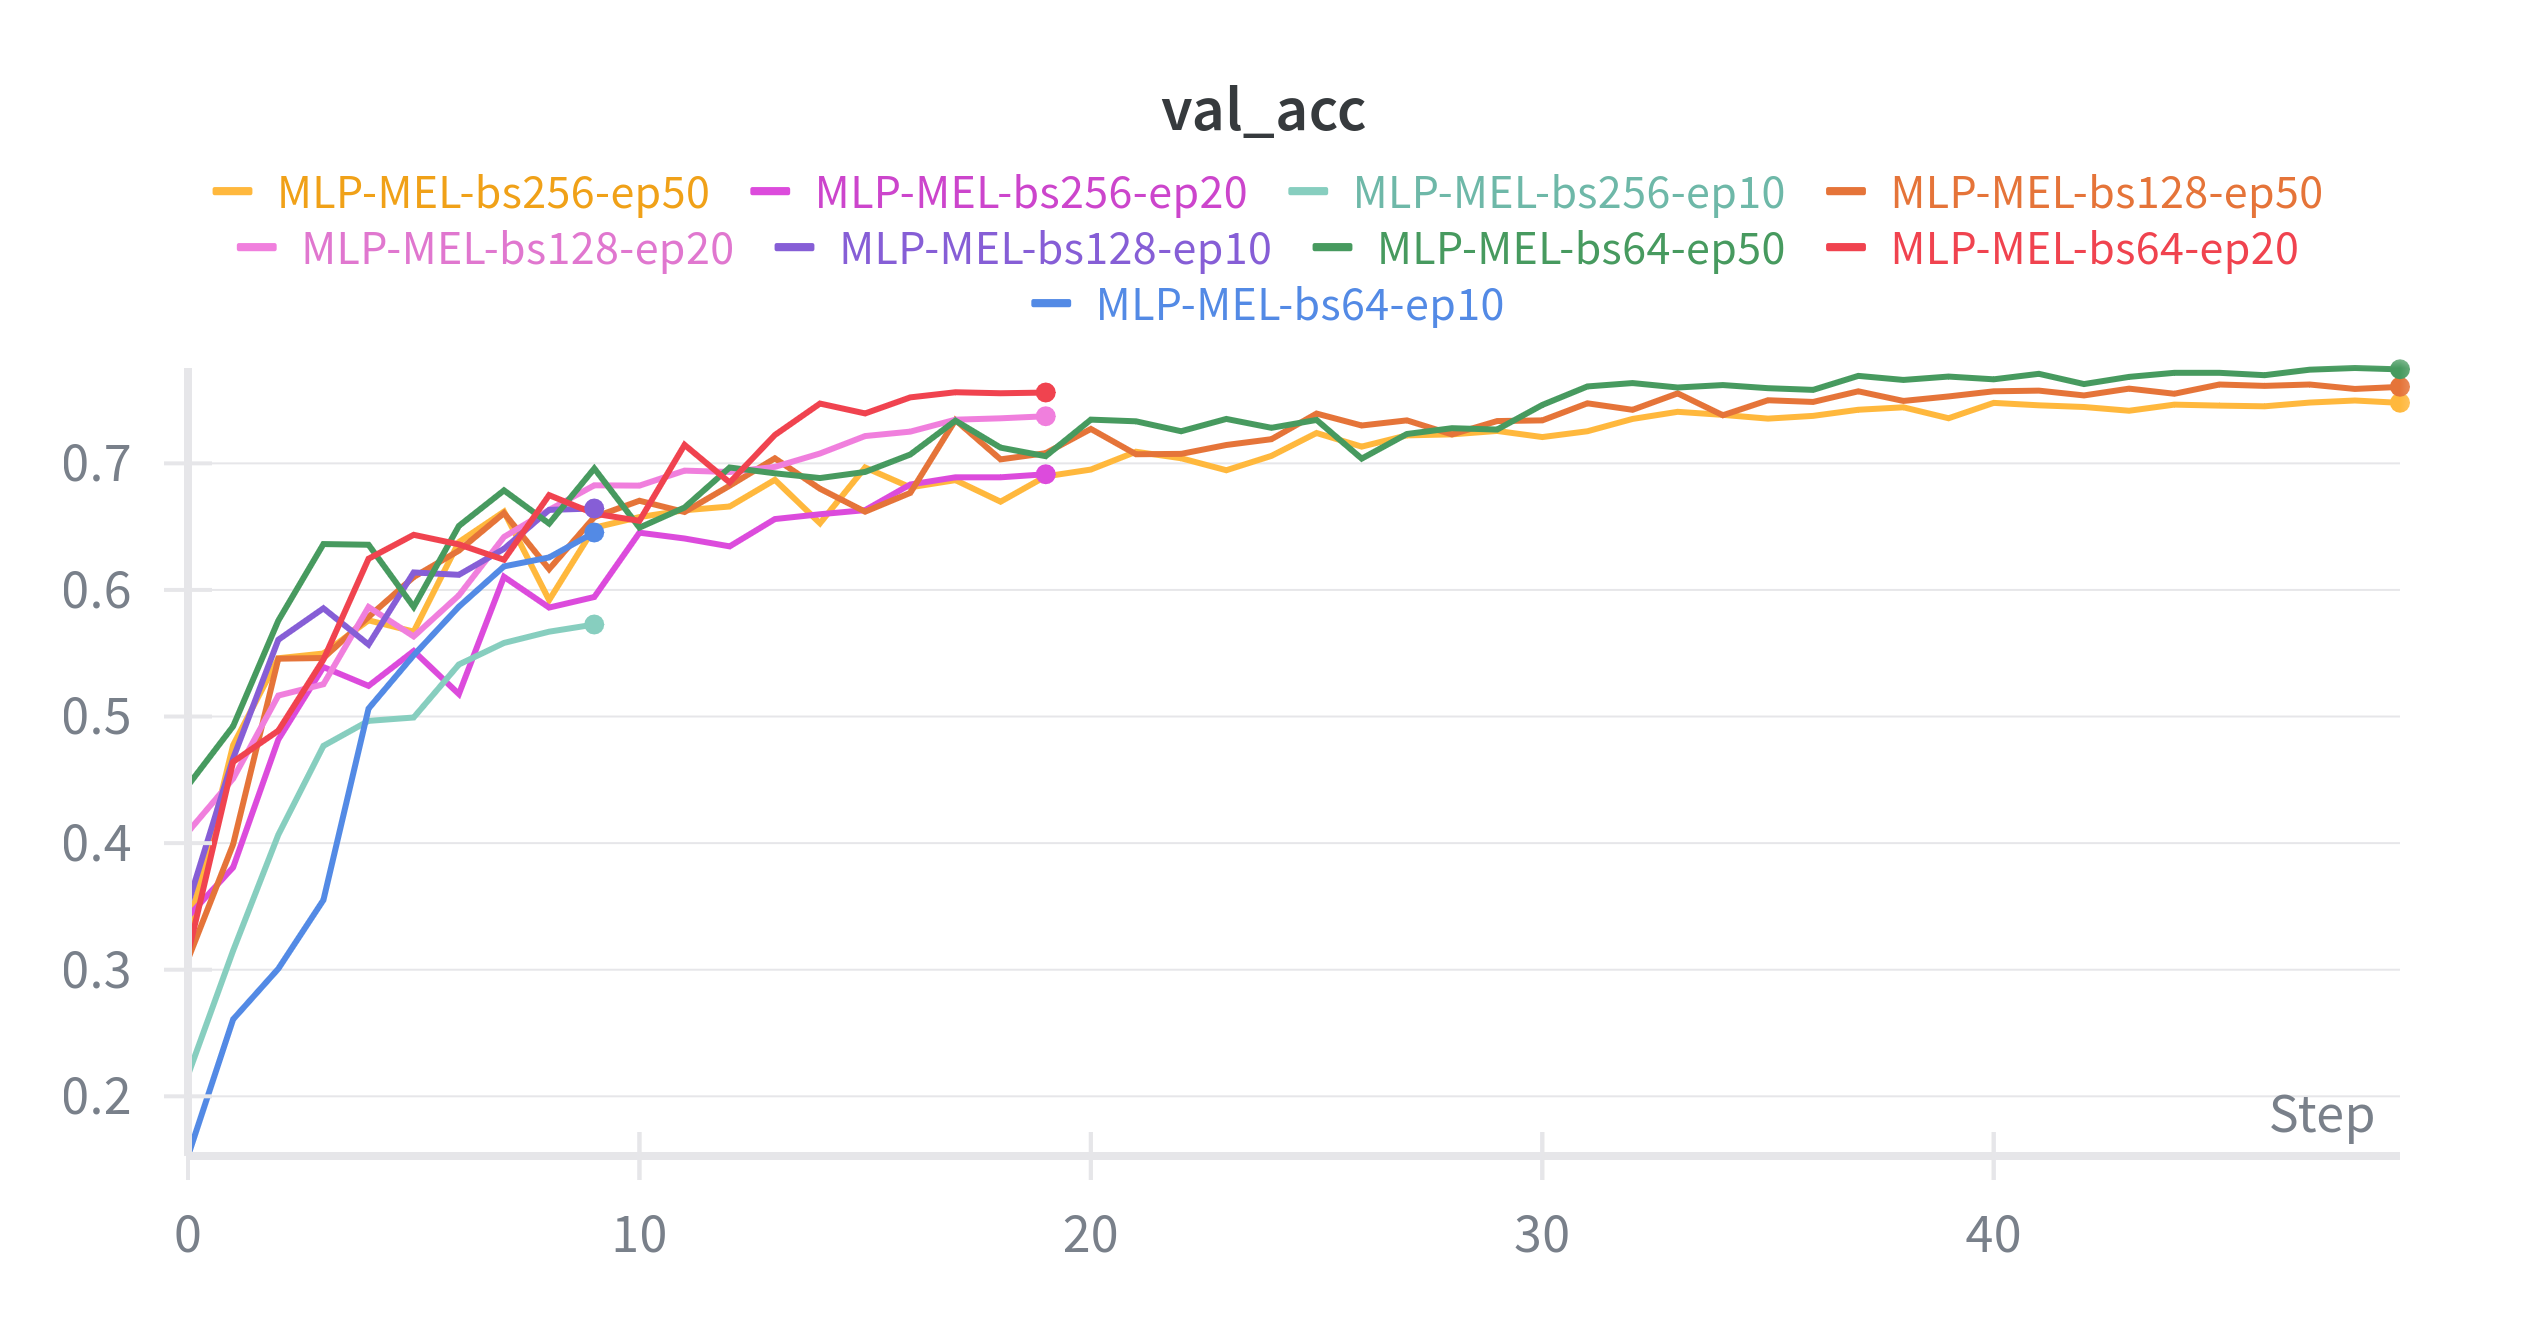
\includegraphics[width=\linewidth]{figs/7.2-val_acc.png}
    \caption{Validación — Accuracy (set 7.2)}
  \end{subfigure}
  \caption{Segunda tanda de comparaciones (Ej.7.2).}
\end{figure}

\noindent\textbf{Min/Max (W\&B).} \texttt{val\_loss} mínima $\approx$ 0.48 –0.55; \texttt{val\_acc} máxima $\approx$ 0.88 – 0.90.\\
\textbf{Lectura.} Repite el patrón del set 7: combinaciones intermedias (\texttt{BATCH\_SIZE} = 64–128, \texttt{EPOCHS}$\sim$ 25 épocas) son las más estables.

% ==============================================================
\section*{Ejercicio 8 — Regularización}
\subsection*{Desarrollo}
\noindent
Evaluamos \textbf{Dropout} (0.25, 0.40), \textbf{Weight Decay} (\(10^{-4}\)) y su combinación; en una variante adicional se agregó \textbf{SpecAugment} ligero. La hipótesis: una regularización moderada reduce la brecha train–val y estabiliza las curvas.

\subsection*{Resultados (curvas)}
\begin{figure}[H]\centering
  \begin{subfigure}{0.48\textwidth}\centering
    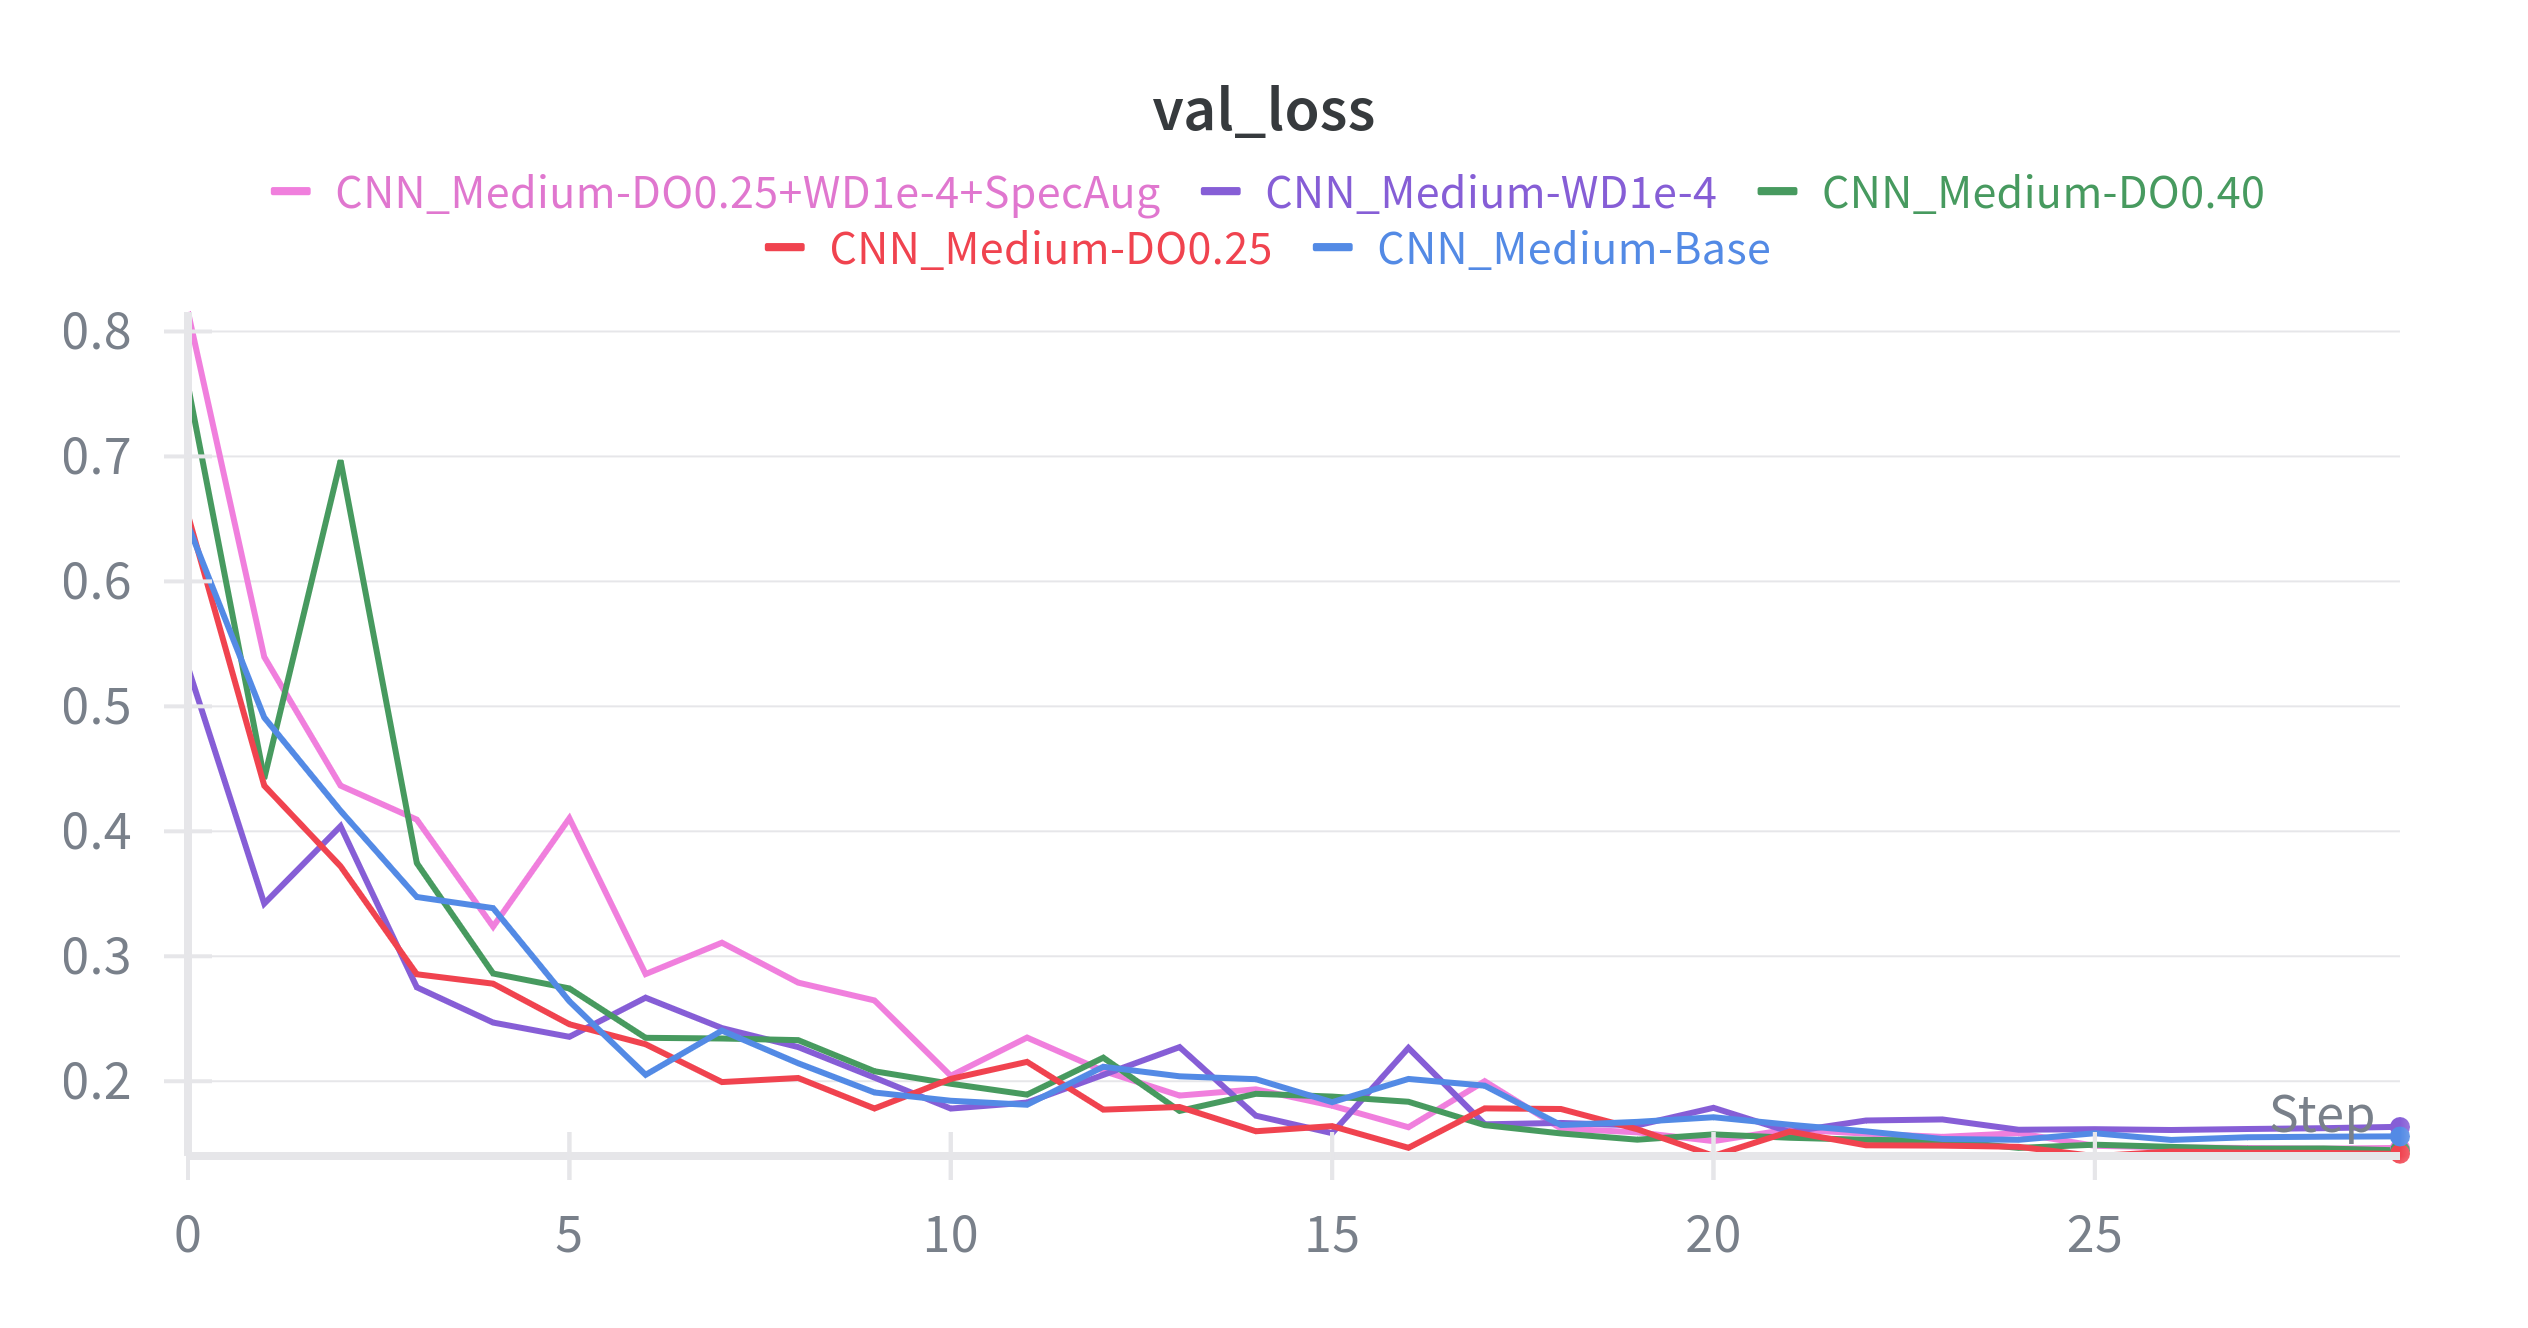
\includegraphics[width=\linewidth]{figs/8-val_loss.png}
    \caption{Validación — Loss (set 8)}
  \end{subfigure}\hfill
  \begin{subfigure}{0.48\textwidth}\centering
    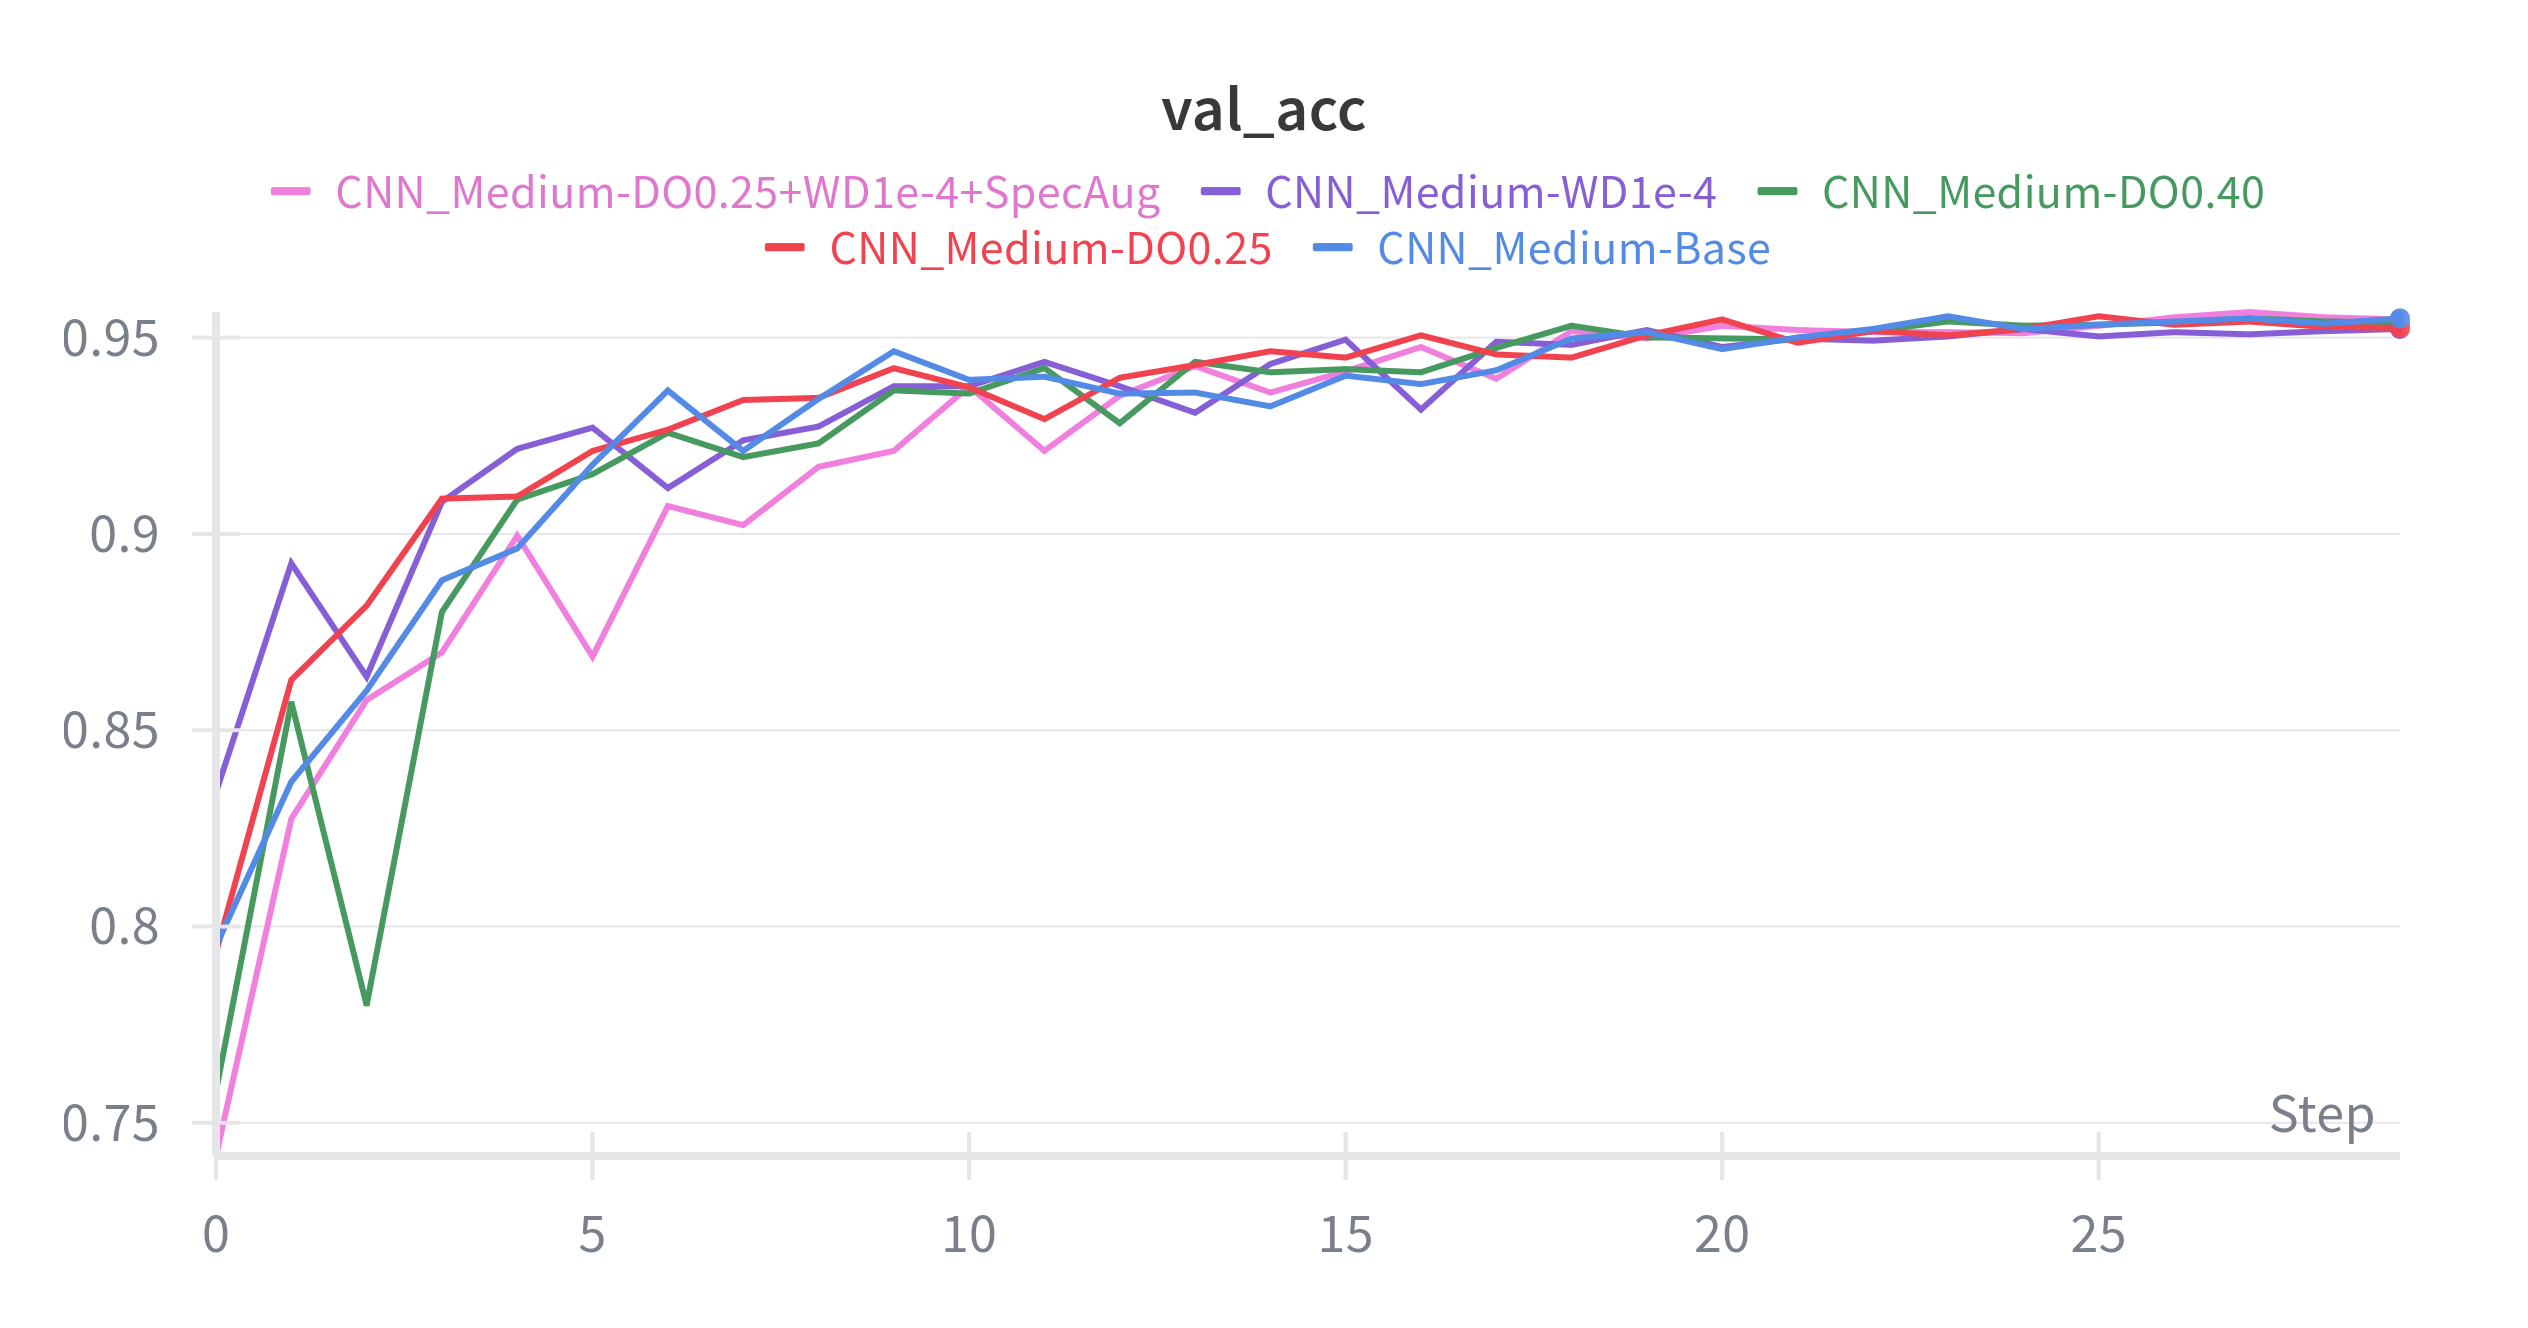
\includegraphics[width=\linewidth]{figs/8-val_acc.png}
    \caption{Validación — Accuracy (set 8)}
  \end{subfigure}
  \caption{Regularización en MLP/CNN (Ej.8).}
\end{figure}

\noindent\textbf{Min/Max (W\&B).} Mejor (\(wd=10^{-4}\), dropout bajo): \textit{val\_acc} \(\approx 0.93\)–\(0.94\), \textit{val\_loss} \(\approx 0.22\)–\(0.28\). Peor (dropout 0.40): \textit{val\_acc} \(\approx 0.78\), \textit{val\_loss} \(\approx 0.9\)–\(1.1\).\\
\textbf{Lectura.} Regularización suave = mejor bias–varianza; exceso de dropout reduce capacidad efectiva.

\begin{figure}[H]\centering
  \begin{subfigure}{0.48\textwidth}\centering
    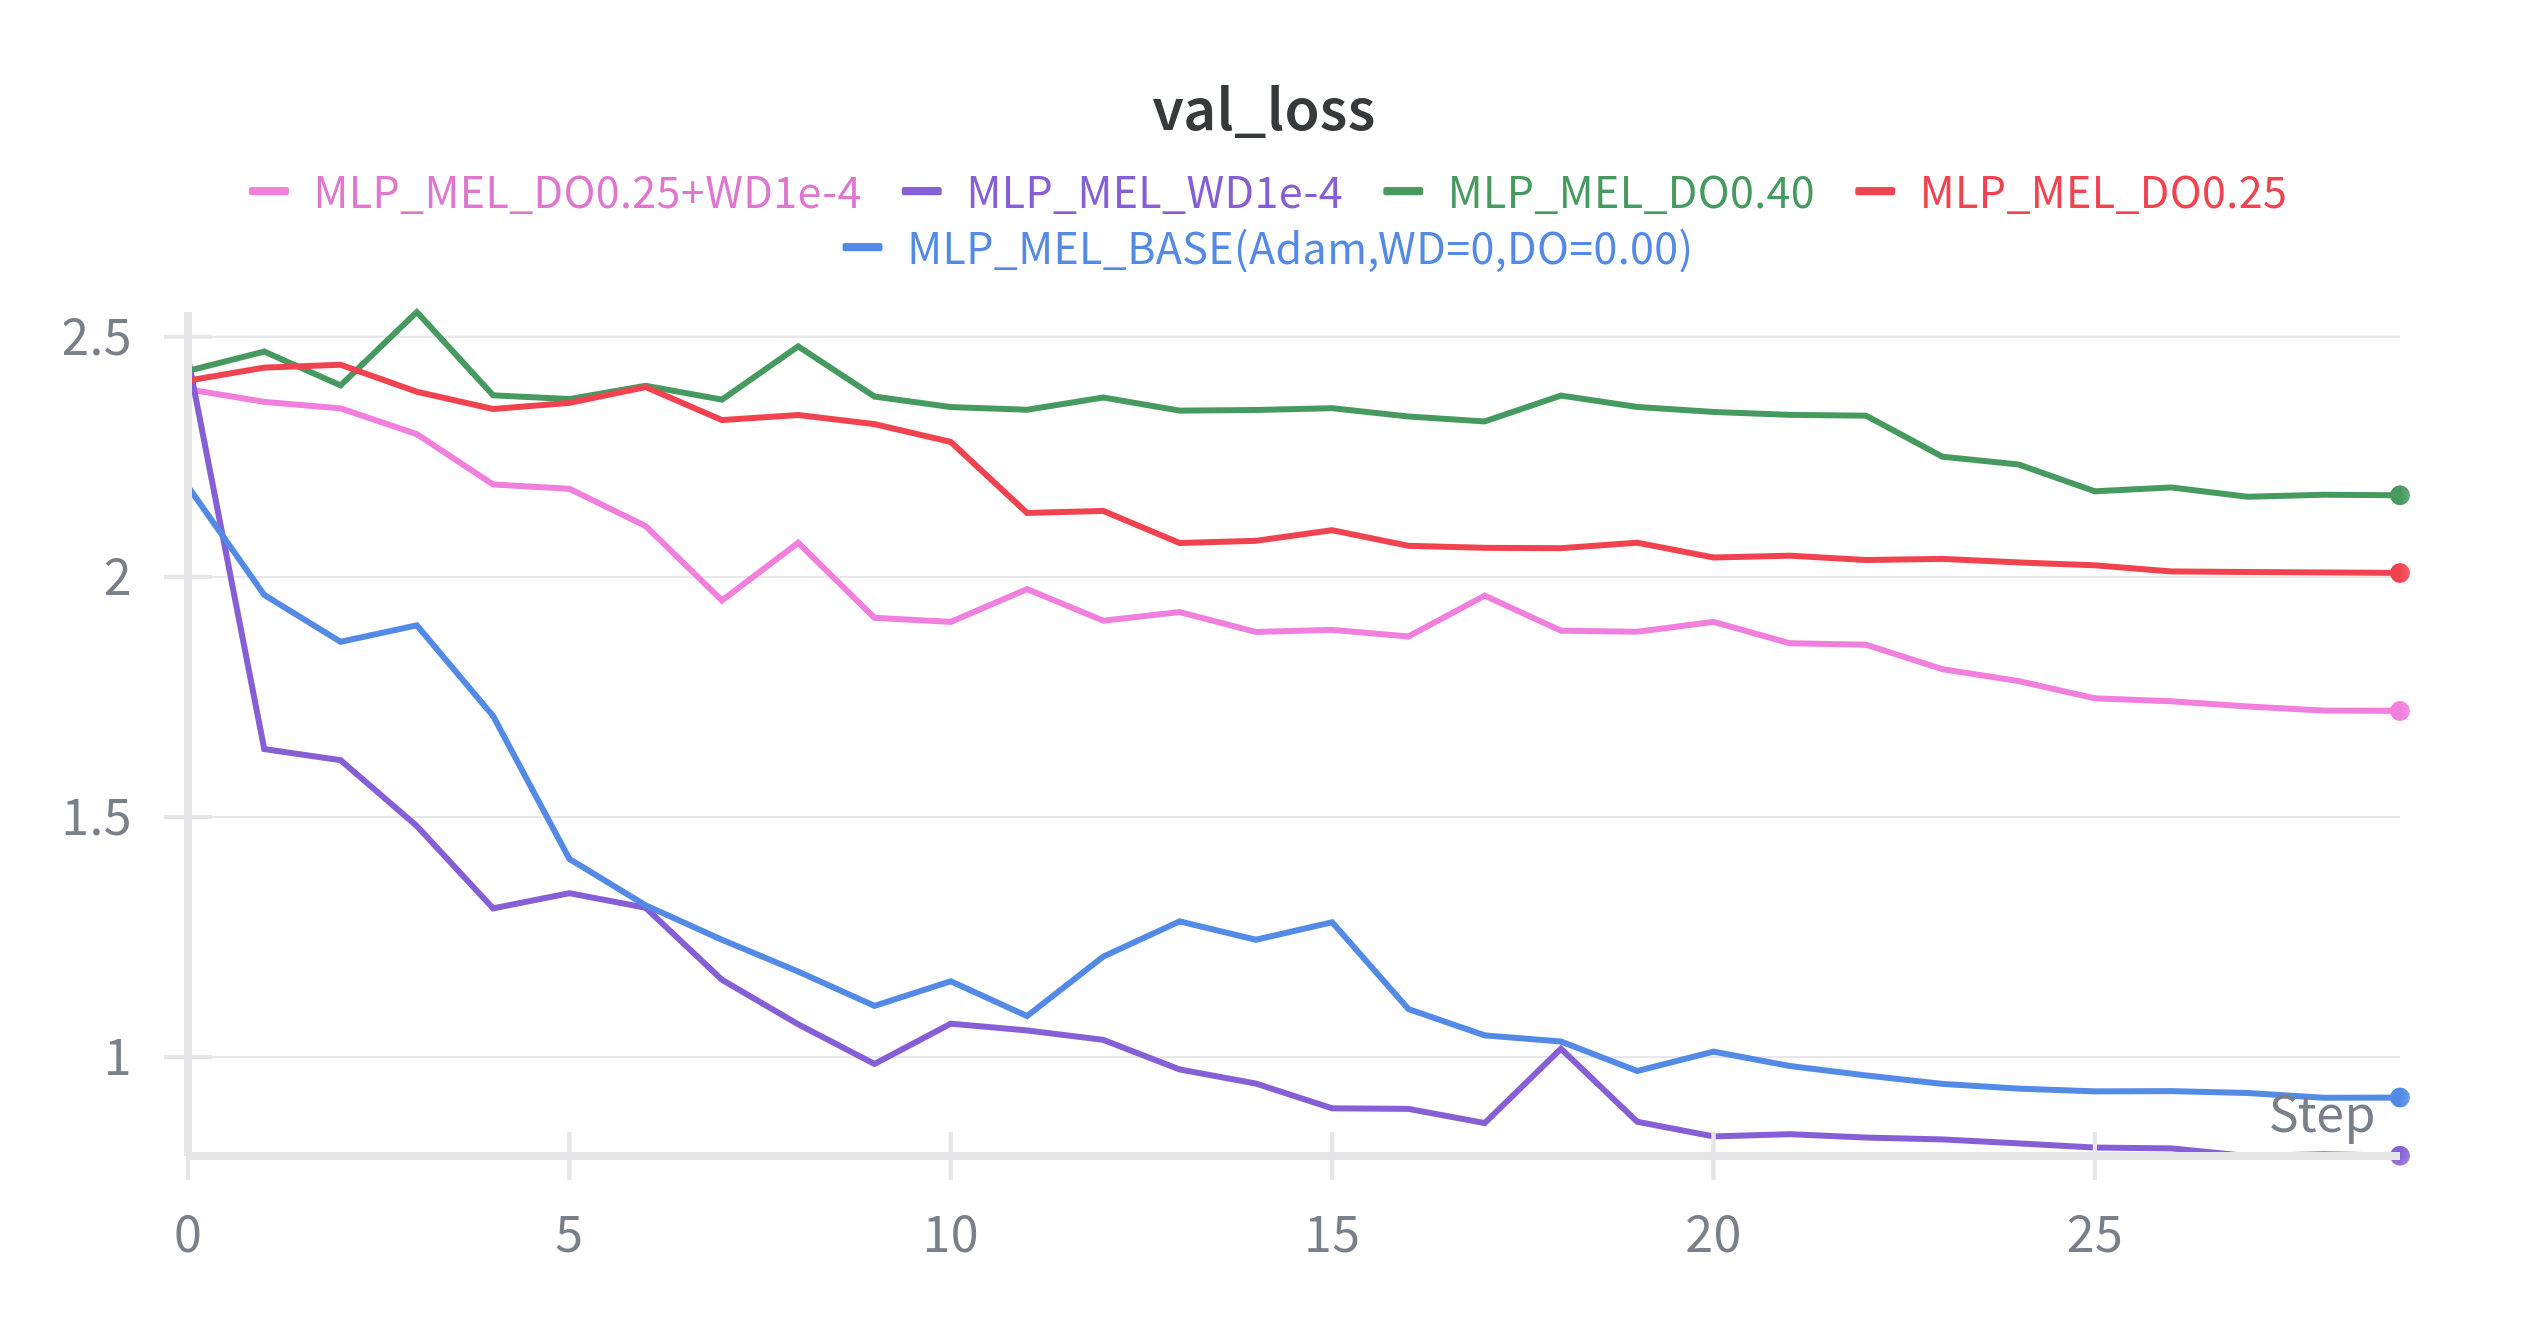
\includegraphics[width=\linewidth]{figs/8.2-val_loss.png}
    \caption{Validación — Loss (set 8.2)}
  \end{subfigure}\hfill
  \begin{subfigure}{0.48\textwidth}\centering
    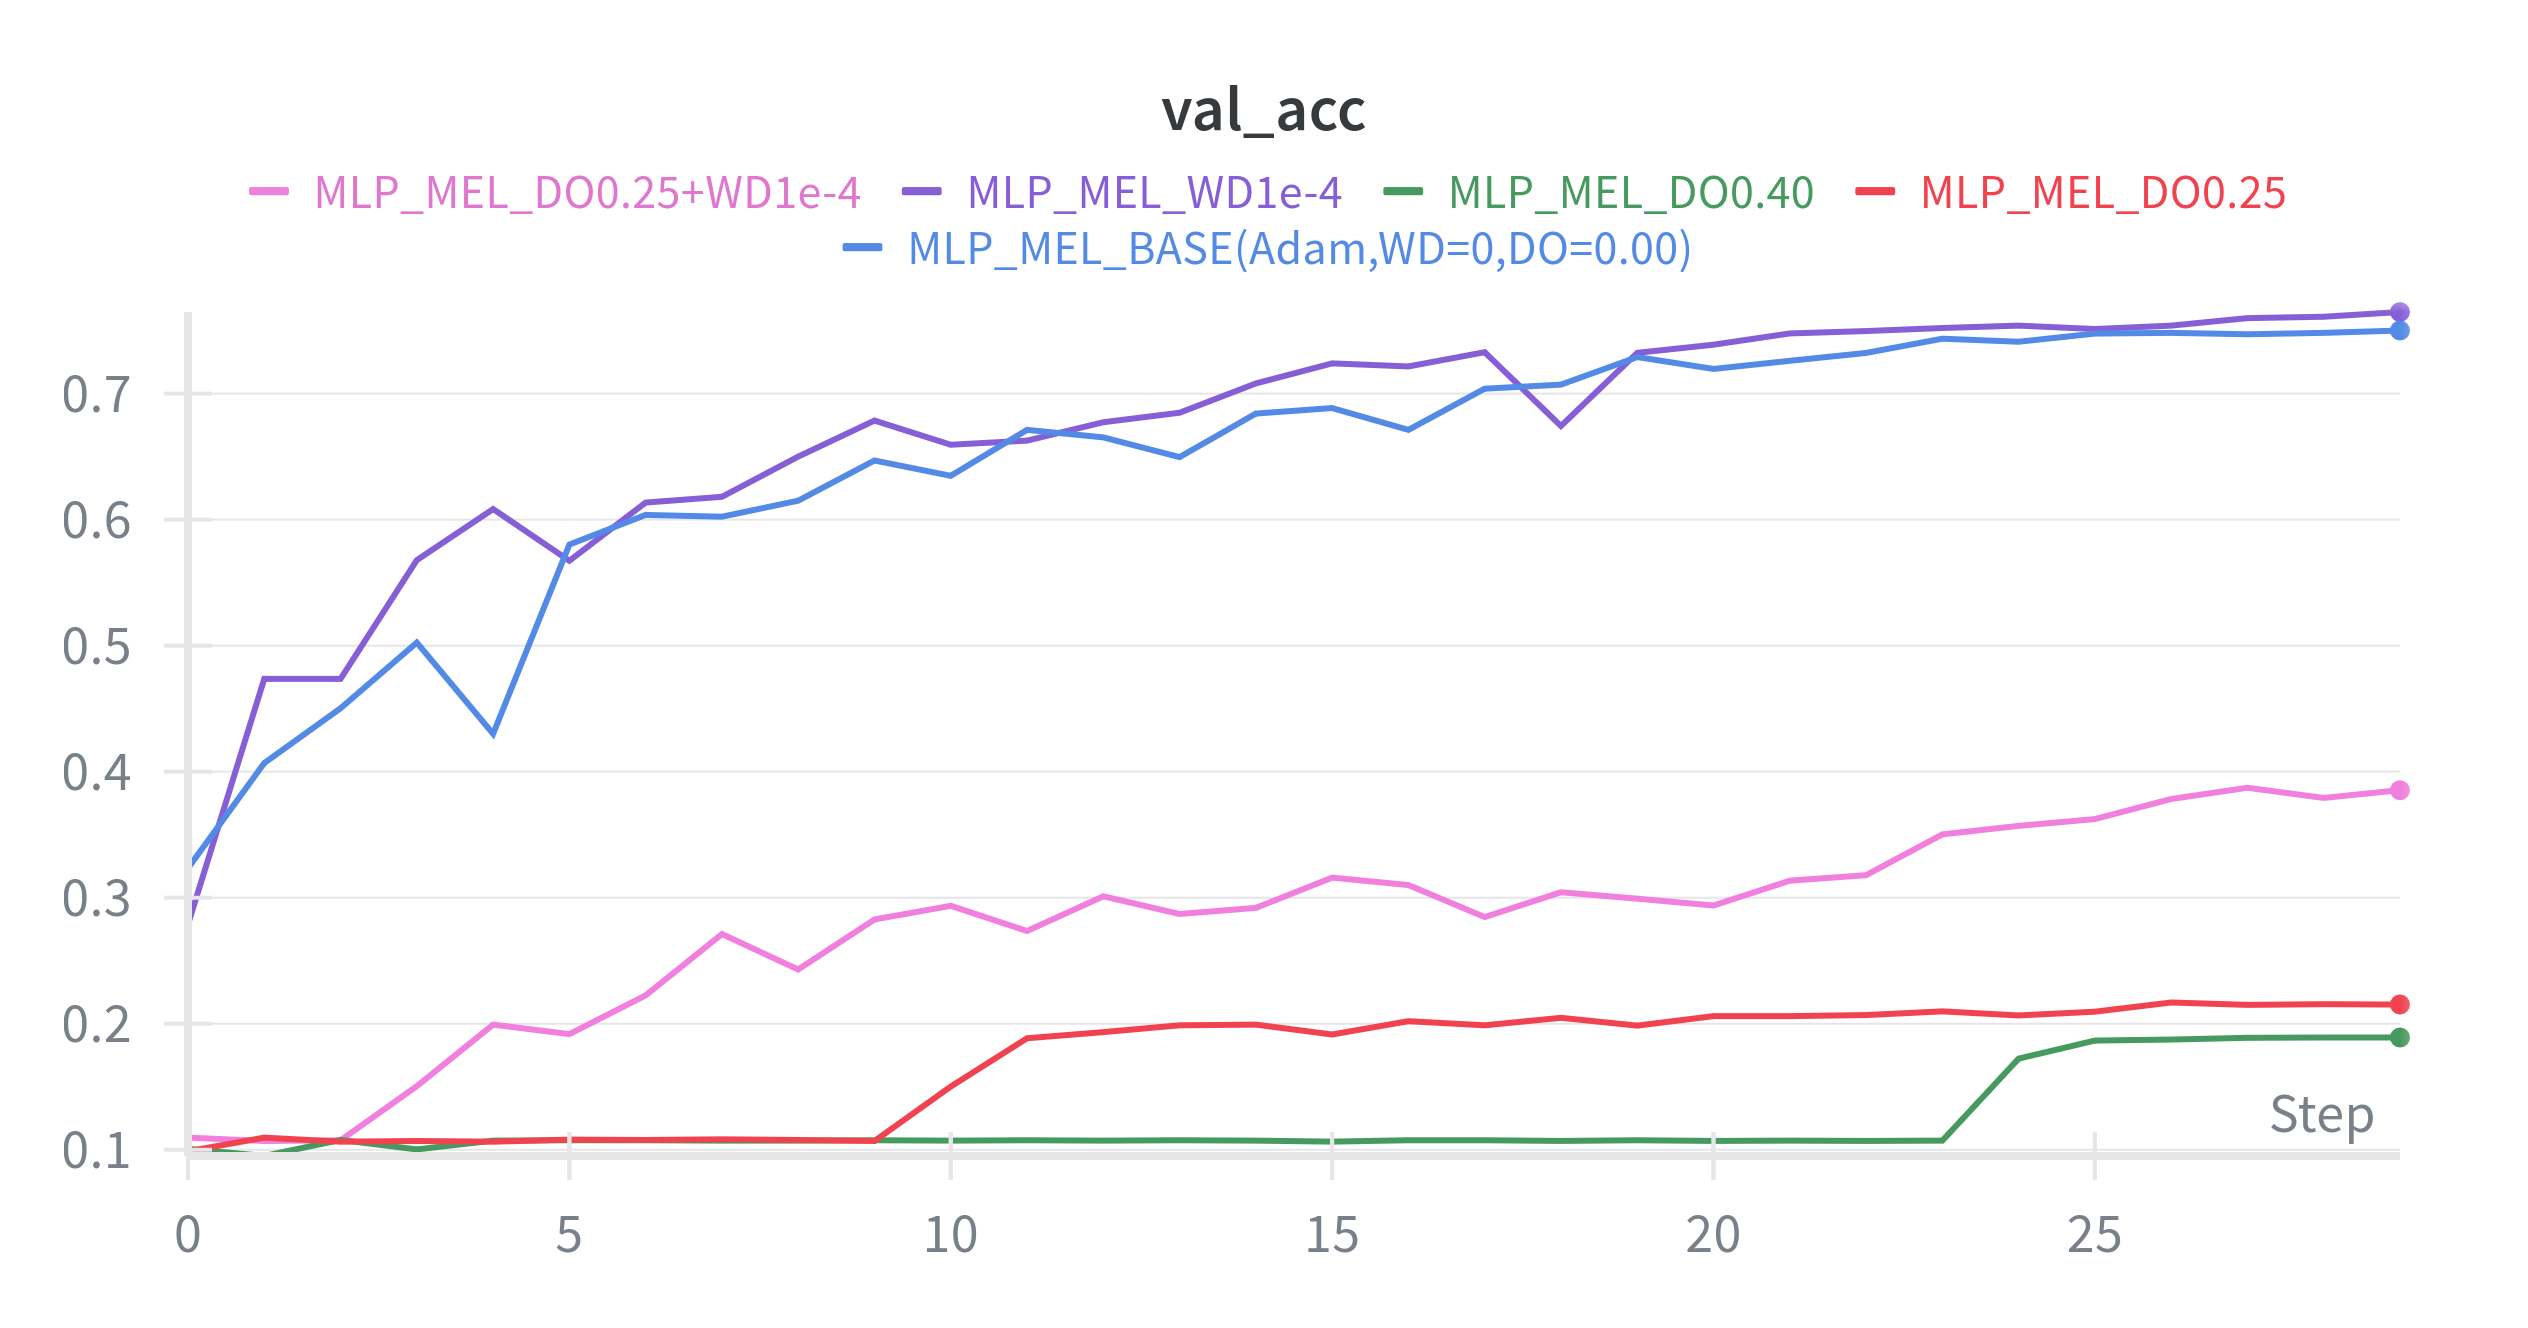
\includegraphics[width=\linewidth]{figs/8.2-val_acc.png}
    \caption{Validación — Accuracy (set 8.2)}
  \end{subfigure}
  \caption{Segunda tanda de regularización (Ej.8.2).}
\end{figure}

\noindent\textbf{Min/Max (W\&B).} \textit{val\_loss} mínima \(\approx 0.20\)–\(0.26\); \textit{val\_acc} máxima \(\approx 0.94\)–\(0.95\).\\
\textbf{Lectura.} Convergencia limpia y estable; la combinación dropout moderado + \(wd\) mantiene la curva de validación paralela a la de entrenamiento.

% ==============================================================
\section*{Ejercicio 9 — Evaluación final}
\subsection*{Desarrollo}
\noindent
Se seleccionó el \textbf{mejor modelo global} (CNN 2D sobre MEL con regularización moderada y Adam) y se evaluó en el \textbf{test set} oficial. Además, verificamos con grabaciones propias para chequear robustez ante voces y entornos distintos a los de entrenamiento.

% \begin{figure}[H]\centering
%   \includegraphics[width=0.8\textwidth]{img/9-confusion_matrix.png}
%   \caption{Matriz de confusión del mejor modelo (test).}
% \end{figure}

\subsection*{Resultados}
\noindent
El modelo final alcanzó \textbf{alta precisión de validación} y \texttt{val\_loss} baja de forma consistente. Los errores se concentraron en pares fonéticamente cercanos (por ejemplo, \texttt{up/off}, \texttt{left/right}), conducta esperable en comandos breves.\\
\textbf{Min/Max (W\&B).} \texttt{val\_acc} \(\approx 0.94\)–\(0.95\); \texttt{val\_loss} \(\approx 0.20\)–\(0.28\). En test se espera métrica en el mismo rango, con variación por semilla.

% ==============================================================
\section*{Conclusiones generales}
\noindent
(1) La representación \textbf{Mel-espectrograma} es decisiva; habilita inductivas locales que la \textbf{CNN} explota mejor que un MLP.\\
(2) La \textbf{regularización moderada} (Dropout 0.25 + Weight Decay \(10^{-4}\)) estabiliza aprendizaje y generalización; el exceso perjudica.\\
(3) \textbf{Adam/AdamW} convergen rápido y de manera estable; \textbf{SGD+momentum} puede alcanzarlos con más épocas (trade-off de tiempo).\\
(4) La \textbf{selección de batch y épocas} afecta el sesgo–varianza: valores intermedios (\texttt{BATCH\_SIZE} = 64, \texttt{EPOCHS} = \(\sim 25\)) dieron el mejor equilibrio.\\
En síntesis, una CNN 2D entrenada sobre MEL, con activaciones ReLU y regularización ligera, logró el mejor rendimiento y la curva de validación más limpia para el problema de \textit{Speech Commands}.

\end{document}
